\documentclass[12pt]{report}

\usepackage[utf8]{inputenc}
\usepackage[T1]{fontenc}
\usepackage{textcomp}
\usepackage[french, english]{babel}
\usepackage{algorithm}
\usepackage{algpseudocode}
\usepackage{graphicx}
\usepackage{hyperref}
\usepackage{svg}

\usepackage{tikz}
\usepackage{pgfplots}
\usepgfplotslibrary{external} 
\tikzexternalize
\newcommand*\circled[1]{\tikz[baseline=(char.base)]{
            \node[shape=circle,draw,inner sep=0.8pt] (char) {#1};}}


\usepackage[hyperref=true,%
            url=false,%
            isbn=false,%
            style=numeric,%
            maxcitenames=3,%
            maxbibnames=100,%
            block=none]{biblatex}

\bibliography{../src/bib/OS.bib}
\bibliography{../src/bib/Flow-Based Programming.bib}
\bibliography{../src/bib/Functional Programming-Functional Reactive Programming.bib}
\bibliography{../src/bib/Stream.bib}
\bibliography{../src/bib/Dataflow.bib}
\bibliography{../src/bib/Web & Social Networks.bib}
\bibliography{../src/bib/Others.bib}
\bibliography{../src/bib/Actor Model.bib}
\bibliography{../src/bib/Misc.bib}
\bibliography{../src/bib/Parallelisation.bib}
\bibliography{../src/bib/Others.bib}
\bibliography{../src/bib/Distributed Systems.bib}
\bibliography{../src/bib/sigproc.bib}

\usepackage{color}
\usepackage{listings}

% Configuration de la coloration syntaxique du code
\definecolor{bleugris}{rgb}{.2,.4,.5}
\definecolor{colKeys}{rgb}{0,0,1}
\definecolor{colIdentifier}{rgb}{0,0,0}
\definecolor{colComments}{rgb}{0,0.5,1}
\definecolor{colString}{rgb}{0.6,0.1,0.1}

\newcommand{\nClass}[1]{{\color{bleugris}{\textsl{\textbf{#1}}}}}
\newcommand{\nParameter}[1]{{\color{gray}{\textbf{#1}}}}
\newcommand{\nMethod}[1]{{\color{gray}{\textbf{#1}}}}
\newcommand{\nConstant}[1]{\texttt{\uppercase{#1}}}
\newcommand{\nKeyword}[1]{\textsl{\textbf{#1}}}


\definecolor{lightgray}{rgb}{.9,.9,.9}
\definecolor{darkgray}{rgb}{.4,.4,.4}
\definecolor{purple}{rgb}{0.65, 0.12, 0.82}
\lstdefinelanguage{JavaScript}{
  keywords={break, case, catch, continue, debugger, default, delete, do, else, false, finally, for, function, if, in, instanceof, new, null, return, switch, this, throw, true, try, typeof, var, void, while, with},
  morecomment=[l]{//},
  morecomment=[s]{/*}{*/},
  morestring=[b]',
  morestring=[b]",
  ndkeywords={class, export, boolean, throw, implements, import, this},
  keywordstyle=\color{blue}\bfseries,
  ndkeywordstyle=\color{darkgray}\bfseries,
  identifierstyle=\color{black},
  commentstyle=\color{purple}\ttfamily,
  stringstyle=\color{red}\ttfamily,
  sensitive=true
}

\newcommand{\userlstset}[1]{
  \lstset{ %
    language=#1,                   % choose the language of the code
    identifierstyle=\color{colIdentifier},%
    basicstyle=\ttfamily\scriptsize, %
    keywordstyle=\color{colKeys},%
    stringstyle=\color{colString},%
    commentstyle=\color{colComments},%
    numberstyle=\tiny,              % the size of the fonts that are used for the line-numbers
    numbers=left,                   % where to put the line-numbers
    stepnumber=1,                   % the step between two line-numbers. If it is 1 each line will be numbered
    numbersep=5pt,                  % how far the line-numbers are from the code
    backgroundcolor=\color{white},  % choose the background color. You must add \usepackage{color}
    showspaces=false,               % show spaces adding particular underscores
    showstringspaces=false,         % underline spaces within strings
    showtabs=false,                 % show tabs within strings adding particular underscores
    %frame=single,                  % adds a frame around the code
    tabsize=2,                      % sets default tabsize to 2 spaces
    captionpos=b,                   % sets the caption-position to bottom
    breaklines=true,                % sets automatic line breaking
    breakautoindent = true,         %
    breakatwhitespace=false,        % sets if automatic breaks should only happen at whitespace
    escapeinside={\@}{\@},         % if you want to add a comment within your code
    % texcl=true
  } %
}

\newcommand{\ic}[1]{\lstinline|#1|}

\lstnewenvironment{code}[1][JavaScript]{%
  \userlstset{#1}%
}{%
}
\usepackage{marginnote}
\usepackage{xcolor}
\usepackage{pifont}

\definecolor{todo}{rgb}{0.9,0.5,0.5}
\definecolor{text}{gray}{0.8}
\definecolor{red}{rgb}{1,0,0.29}
\definecolor{gray1}{rgb}{.70,.70,.70}
\definecolor{gray2}{rgb}{.75,.75,.75}
\definecolor{gray3}{rgb}{.80,.80,.80}
\definecolor{gray4}{rgb}{.85,.85,.85}
\definecolor{gray5}{rgb}{.90,.90,.90}
\definecolor{gray6}{rgb}{.95,.95,.95}

\definecolor{RED}{RGB}{255, 0, 73}
\definecolor{GREEN}{RGB}{190, 255, 0}

\newcommand{\TODO}[1]{%
  % \marginpar
  {
    \textcolor{todo}{\bf TODO}
    \textcolor{text}{#1}
  }
}

\newcommand{\ind }{%
  \hspace{4ex}%
}

\newcommand{\comment}[1]{%
  \textcolor{text}{#1}%
}

\newcommand{\nt}[1]{%
  \textcolor{red}{*}%
  \marginpar{\textcolor{red}{\fontencoding{U}\fontfamily{futs}\selectfont\char 66\relax}\vspace{3mm}\\
  \tiny{\textcolor{text}{#1}}}%
}

\newcommand{\illustration}[1]{%
% \reversemarginpar%
% \marginpar{\tiny{illustration:\\#1}}%
% \normalmarginpar%
}

\newcommand{\ftnt}[1]{%
  \footnote{\small{\url{#1}}}%
}

\newcommand{\cit}[2]{%
  \noindent%
  \textit{{\secfont\fontsize{45pt}{10pt}\selectfont``}\LARGE{#1}{''}}\\[-5pt]%
  \begin{flushright}%
  --- #2%
  \end{flushright}%
  \vspace{30pt}
}


\newcommand*\rot{\rotatebox{90}}

\newcommand\lab[1]{%
  \rotatebox{90}{\parbox{3cm}{\raggedright #1}}%
}

\newlength\replength
\newcommand\repfrac{.33}
\newcommand\dashfrac[1]{\renewcommand\repfrac{#1}}
\setlength\replength{4.5pt}
\newcommand\rulewidth{1.6pt}

\newcommand\tdotfill[1][\repfrac]{\cleaders\hbox to \replength{%
  \smash{\raisebox{\arraystretch\dimexpr\ht\strutbox-.1ex\relax}{.}}}\hfill}
\newcommand\tabdotline{%
  \makebox[0pt][r]{\makebox[\tabcolsep]{\tdotfill\hfil}}\tdotfill\hfil%
  \makebox[0pt][l]{\makebox[\tabcolsep]{\tdotfill\hfil}}%
  \\[-\arraystretch\dimexpr\ht\strutbox+\dp\strutbox\relax]%
}

\newcommand{\separator}{%
\vspace{20pt}%
\begin{center}%
% \hrulefill%
\begin{tikzpicture}%
\draw (0,0) -- (0.2,0.2);%
\draw (0,0.2) -- (0.2,0);%
\end{tikzpicture}%
% \hrulefill%
\end{center}%
\vspace{10pt}%
}


% \newcommand{\V}{ \textcolor{green}{\ding{51}} }
% \newcommand{\X}{ \textcolor{red}{\ding{53}} }
% \newcommand{\U}{ \textcolor{gray}{?} }
% \newcommand{\J}{ \textcolor{cyan}{\textbf{+}} }
% \newcommand{\M}{ \textcolor{orange}{--} }

\newlength\callStackIndentation
\newcommand{\level}[1]{%
  \setlength\callStackIndentation{2em}%
  \hspace*{#1\callStackIndentation}%
}

\newcommand*{\circled}[1]{\tikz[baseline=(char.base)]{
            \node[shape=circle,draw,inner sep=0.8pt] (char) {#1};}}

\newcommand*{\dotcircled}[1]{\tikz[baseline=(char.base)]{
            \node[shape=circle,draw,line cap=round, dash pattern=on 0pt off 3pt,inner sep=0.8pt] (char) {#1};}}

\newcommand*{\rate}[1]{\tikz[baseline=(char.base)]{
            \colorlet{tmpcolor}{green!\the\numexpr#1*20!red}
            \node[shape=circle,inner sep=0.8pt, fill=tmpcolor] (char) {\textcolor{white}{\textbf#1}};}}

\setcounter{secnumdepth}{3}
\setcounter{tocdepth}{3}

\begin{document}

\title{Operating Systems mutations, how and why integrate the user in the digital era ?\\\comment{TODO change title ?}}
\author{Etienne Brodu}

\maketitle

\renewcommand{\glyph}{\iconfont{\XeTeXglyph287}}
\chapter{Implementations} \label{chapter5}
\minitoc
\eject
The transformation allowed by the equivalence from an event-driven program into a distributed network of fluxions is implemented incrementally into two compilers, as presented in figure \ref{fig:roadmap}.
Each compilers is divided into two steps, the identification of the rupture points separating the stages of the pipeline, and the isolation of these stages.
% This chapter presents the technical implementations of these two steps in the transformation from the event-driven execution model to the pipeline architecture
% , the transformation described in the previous chapter was implemented incrementally in two compilers.

\begin{figure}[h!]%
  \textfig{%
    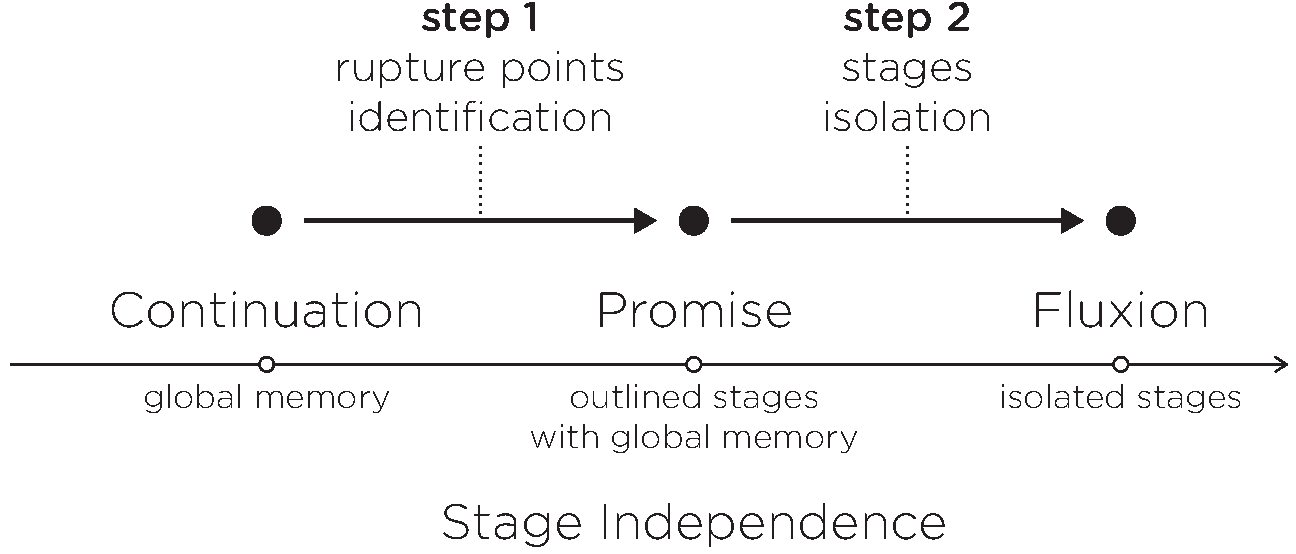
\includegraphics[width=0.7\textwidth]{../resources/roadmap.pdf}%
    \caption{Roadmap}%
    \label{fig:roadmap}%
  }%
\end{figure}

The first compiler focuses on the identification of simple chains of causality between continuations to transform these chains into Promises.
% the transformation from continuations to Promises.
% It focuses on the identification of the chains of causality in continuations.
However, promises are more expressive than the simple chaining of causal sequentiality.
% They force another control over the execution flow.
% According to the outcome of the operation, they call one function to continue the execution with the result, or another to handle errors.
% This conditional execution is indivisible from the Promise specification.
% Promises impose a convention on how to hand back the outcome of the deferred computation, while classic continuations leave this conditional execution to the developer.
Moreover, they impose a different convention than continuations on how to hand back the outcome and errors of the deferred computation.
This difference brings unnecessary complexity to the identification of chains.
To rule out this difference between continuations and Promises, before introducing the first compiler, section \ref{chapter5:due} introduces a simpler specification to Promise, called Due.

The second compiler detects all the chains of causality between continuations and encapsulate them in fluxions.
It isolates the fluxions when possible to allow the parallelism required for efficiency.
This second compilers is introduced in section \ref{chapter5:flx}.

\renewcommand{\glyph}{\iconfont{\XeTeXglyph287}}
\chapter{Implementations} \label{chapter5}
\minitoc
\eject
The transformation allowed by the equivalence from an event-driven program into a distributed network of fluxions is implemented incrementally into two compilers, as presented in figure \ref{fig:roadmap}.
Each compilers is divided into two steps, the identification of the rupture points separating the stages of the pipeline, and the isolation of these stages.
% This chapter presents the technical implementations of these two steps in the transformation from the event-driven execution model to the pipeline architecture
% , the transformation described in the previous chapter was implemented incrementally in two compilers.

\begin{figure}[h!]%
  \textfig{%
    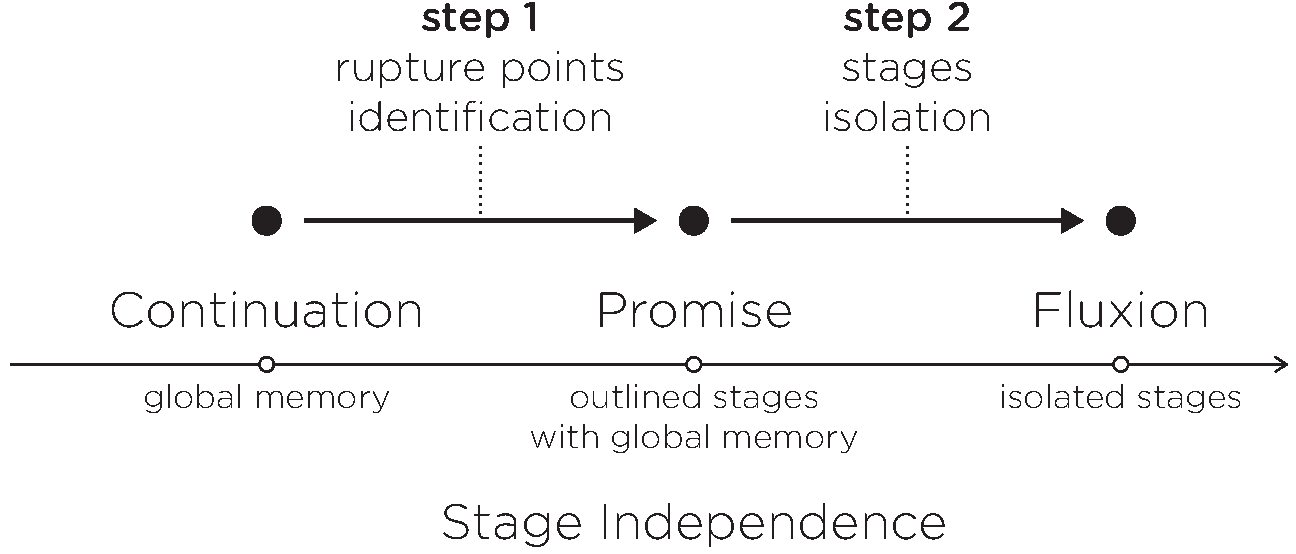
\includegraphics[width=0.7\textwidth]{../resources/roadmap.pdf}%
    \caption{Roadmap}%
    \label{fig:roadmap}%
  }%
\end{figure}

The first compiler focuses on the identification of simple chains of causality between continuations to transform these chains into Promises.
% the transformation from continuations to Promises.
% It focuses on the identification of the chains of causality in continuations.
However, promises are more expressive than the simple chaining of causal sequentiality.
% They force another control over the execution flow.
% According to the outcome of the operation, they call one function to continue the execution with the result, or another to handle errors.
% This conditional execution is indivisible from the Promise specification.
% Promises impose a convention on how to hand back the outcome of the deferred computation, while classic continuations leave this conditional execution to the developer.
Moreover, they impose a different convention than continuations on how to hand back the outcome and errors of the deferred computation.
This difference brings unnecessary complexity to the identification of chains.
To rule out this difference between continuations and Promises, before introducing the first compiler, section \ref{chapter5:due} introduces a simpler specification to Promise, called Due.

The second compiler detects all the chains of causality between continuations and encapsulate them in fluxions.
It isolates the fluxions when possible to allow the parallelism required for efficiency.
This second compilers is introduced in section \ref{chapter5:flx}.

\renewcommand{\glyph}{\iconfont{\XeTeXglyph287}}
\chapter{Implementations} \label{chapter5}
\minitoc
\eject
The transformation allowed by the equivalence from an event-driven program into a distributed network of fluxions is implemented incrementally into two compilers, as presented in figure \ref{fig:roadmap}.
Each compilers is divided into two steps, the identification of the rupture points separating the stages of the pipeline, and the isolation of these stages.
% This chapter presents the technical implementations of these two steps in the transformation from the event-driven execution model to the pipeline architecture
% , the transformation described in the previous chapter was implemented incrementally in two compilers.

\begin{figure}[h!]%
  \textfig{%
    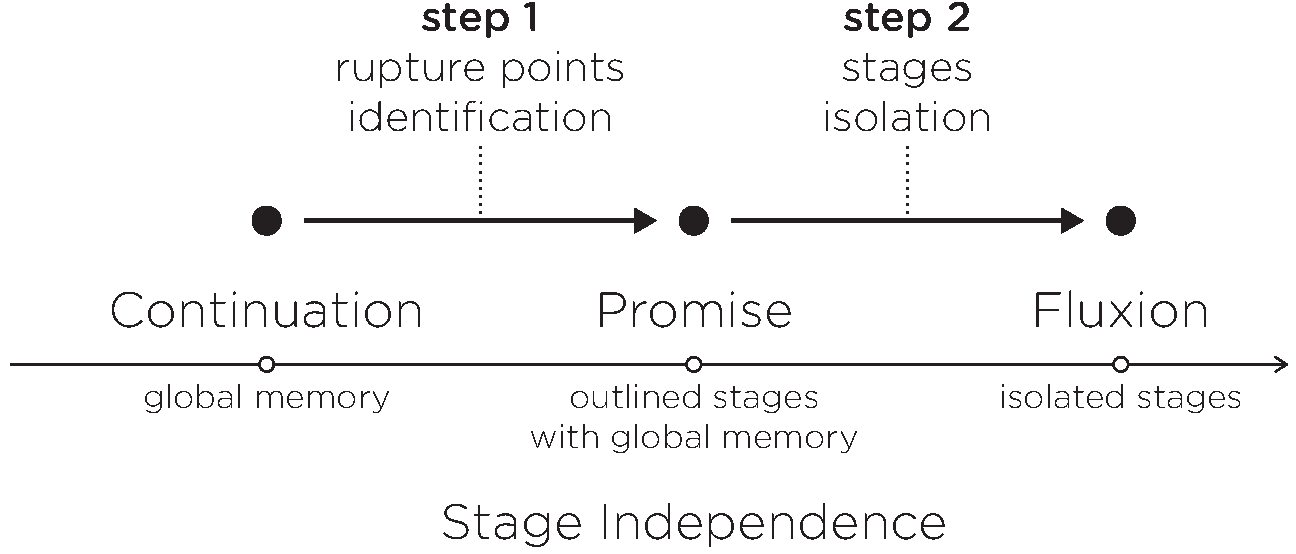
\includegraphics[width=0.7\textwidth]{../resources/roadmap.pdf}%
    \caption{Roadmap}%
    \label{fig:roadmap}%
  }%
\end{figure}

The first compiler focuses on the identification of simple chains of causality between continuations to transform these chains into Promises.
% the transformation from continuations to Promises.
% It focuses on the identification of the chains of causality in continuations.
However, promises are more expressive than the simple chaining of causal sequentiality.
% They force another control over the execution flow.
% According to the outcome of the operation, they call one function to continue the execution with the result, or another to handle errors.
% This conditional execution is indivisible from the Promise specification.
% Promises impose a convention on how to hand back the outcome of the deferred computation, while classic continuations leave this conditional execution to the developer.
Moreover, they impose a different convention than continuations on how to hand back the outcome and errors of the deferred computation.
This difference brings unnecessary complexity to the identification of chains.
To rule out this difference between continuations and Promises, before introducing the first compiler, section \ref{chapter5:due} introduces a simpler specification to Promise, called Due.

The second compiler detects all the chains of causality between continuations and encapsulate them in fluxions.
It isolates the fluxions when possible to allow the parallelism required for efficiency.
This second compilers is introduced in section \ref{chapter5:flx}.

\input{05-implementation/Due/main}
\input{05-implementation/Flx/main}
% \input{05-implementation/Evaluation}

\renewcommand{\glyph}{\iconfont{\XeTeXglyph287}}
\chapter{Implementations} \label{chapter5}
\minitoc
\eject
The transformation allowed by the equivalence from an event-driven program into a distributed network of fluxions is implemented incrementally into two compilers, as presented in figure \ref{fig:roadmap}.
Each compilers is divided into two steps, the identification of the rupture points separating the stages of the pipeline, and the isolation of these stages.
% This chapter presents the technical implementations of these two steps in the transformation from the event-driven execution model to the pipeline architecture
% , the transformation described in the previous chapter was implemented incrementally in two compilers.

\begin{figure}[h!]%
  \textfig{%
    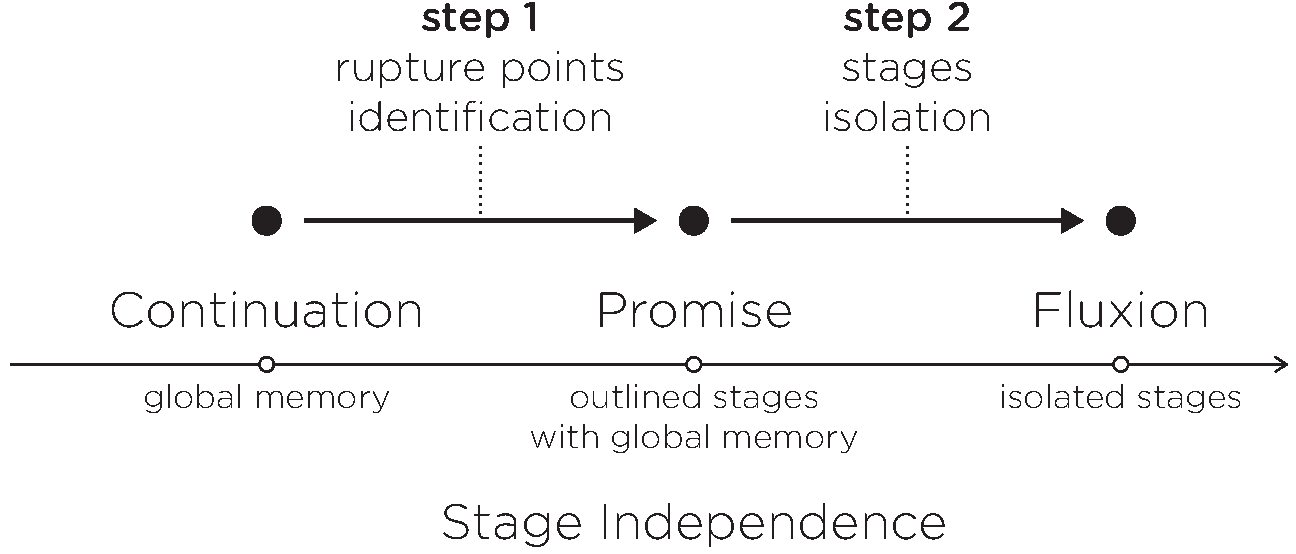
\includegraphics[width=0.7\textwidth]{../resources/roadmap.pdf}%
    \caption{Roadmap}%
    \label{fig:roadmap}%
  }%
\end{figure}

The first compiler focuses on the identification of simple chains of causality between continuations to transform these chains into Promises.
% the transformation from continuations to Promises.
% It focuses on the identification of the chains of causality in continuations.
However, promises are more expressive than the simple chaining of causal sequentiality.
% They force another control over the execution flow.
% According to the outcome of the operation, they call one function to continue the execution with the result, or another to handle errors.
% This conditional execution is indivisible from the Promise specification.
% Promises impose a convention on how to hand back the outcome of the deferred computation, while classic continuations leave this conditional execution to the developer.
Moreover, they impose a different convention than continuations on how to hand back the outcome and errors of the deferred computation.
This difference brings unnecessary complexity to the identification of chains.
To rule out this difference between continuations and Promises, before introducing the first compiler, section \ref{chapter5:due} introduces a simpler specification to Promise, called Due.

The second compiler detects all the chains of causality between continuations and encapsulate them in fluxions.
It isolates the fluxions when possible to allow the parallelism required for efficiency.
This second compilers is introduced in section \ref{chapter5:flx}.

\input{05-implementation/Due/main}
\input{05-implementation/Flx/main}
% \input{05-implementation/Evaluation}

% \subsection{Real test case} \label{chapter5:flx:evaluation}

The compiler is tested on a real application, gifsockets-server\ftnt{https://github.com/twolfson/gifsockets-server}.
This test proves the possibility for an application to be compiled into a network of independent parts.
It shows the current limitations of this isolation and the modifications needed on the application to circumvent them.

\begin{code}[js, caption={Simplified version of gifsockets-server},label={lst:gifsocket}]
var express = require('express'),
    app = express(),
    routes = require('gifsockets-middleware'), //@\label{lst:gifsocket:gif-mw}@
    getRawBody = require('raw-body');

function bodyParser(limit) { //@\label{lst:gifsocket:bodyParser}@
  return function saveBody(req, res, next) { //@\label{lst:gifsocket:saveBody}@
    getRawBody(req, { //@\label{lst:gifsocket:getRawBody}@
      expected: req.headers['content-length'],
      limit: limit
    }, function (err, buffer) { //@\label{lst:gifsocket:callback}@
      req.body = buffer;
      next(); //@\label{lst:gifsocket:next}@
    });
  };
}

app.post('/image/text', bodyParser(1 * 1024 * 1024), routes.writeTextToImages); //@\label{lst:gifsocket:app.post}@
app.listen(8000);
\end{code}

This application, simplified in listing \ref{lst:gifsocket}, is a real-time chat using gif-based communication channels.
It was selected from the evaluation set of the Due compiler because it is simple enough to illustrate this evaluation.
% \cite{Brodu2015}
%  from the \texttt{npm} registry because it depends on \texttt{express}, it is tested, working, and simple enough to illustrate this evaluation.
The server transforms the received text into a gif frame, and pushes it back to a never-ending gif to be displayed on the client.

On line \ref{lst:gifsocket:app.post}, the application registers two functions to process the requests received on the url \texttt{/image/text}.
The closure \texttt{saveBody}, line \ref{lst:gifsocket:saveBody}, returned by \texttt{bodyParser}, line \ref{lst:gifsocket:bodyParser}, and the method \texttt{routes.write\-Text\-To\-Images} from the external module \texttt{gifsockets-\-middleware}, line \ref{lst:gifsocket:gif-mw}.
The closure \texttt{saveBody} calls the asynchronous function \texttt{getRawBody} to get the request body.
Its callback handles the errors, and calls \texttt{next} to continue processing the request with the next function, \texttt{routes.write\-Text\-To\-Images}.

\subsubsection{Compilation} \label{chapter5:flx:evaluation:compilation}

% We compile this application with the compiler
The compilation result is in listing \ref{lst:flx-gifsocket}.
The function call \texttt{app.post}, line \ref{lst:gifsocket:app.post}, is a rupture point.
However, its callbacks, \texttt{bodyParser} and \texttt{routes.write\-Text\-To\-Images} are not declared \textit{in situ}.
They are evaluated as functions only at runtime.
As precised previously, the compiler discards these callbacks to avoid altering the semantic. % by moving or modifying their definition.
% For this reason, the compiler ignores this rupture point, to avoid interfering with the evaluation.

\begin{code}[flx, caption={Compilation result of gifsockets-server},label={lst:flx-gifsocket}]
flx main & express {req}
>> anonymous_1000 [req, next]
  var express = require('express'),
      app = express(),
      routes = require('gifsockets-middleware'), //@\label{lst:flx-gifsocket:gif-mw}@
      getRawBody = require('raw-body');

  function bodyParser(limit) { //@\label{lst:flx-gifsocket:bodyParser}@
    return function saveBody(req, res, next) { //@\label{lst:flx-gifsocket:saveBody}@
      getRawBody(req, { //@\label{lst:flx-gifsocket:getRawBody}@
        expected: req.headers['content-length'], //@\label{lst:flx-gifsocket:req.headers}@
        limit: limit
      }, >> anonymous_1000 [req, next]);
    };
  }

  app.post('/image/text', bodyParser(1 * 1024 * 1024), routes.writeTextToImages); //@\label{lst:flx-gifsocket:app.post}@
  app.listen(8000);

flx anonymous_1000
-> null
  function (err, buffer) { //@\label{lst:flx-gifsocket:callback}@
    req.body = buffer; //@\label{lst:flx-gifsocket:buffer}@
    next(); //@\label{lst:flx-gifsocket:next}@
  }
\end{code}

The compiler detects a rupture point : the function \texttt{get\-Raw\-Body} and its anonymous callback, line \ref{lst:gifsocket:callback}.
It encapsulates this callback in a fluxion named \texttt{anony\-mous\_\-1000}.
The callback is replaced with a stream placeholder to send the message stream to this downstream fluxion.
The variables \texttt{req} and \texttt{next} are appended to this message stream, to propagate their value from the \texttt{main} fluxion to the \texttt{anony\-mous\_\-1000} fluxion.

When \texttt{anony\-mous\_\-1000} is not isolated from the \texttt{main} fluxion, as if they belong to the same group, the compilation result works as expected.
The variables used in the fluxion, \texttt{req} and \texttt{next}, are still shared between the two fluxions.
In this situation fluxions are quite similar to Dues regarding memory shareing.
Our goal is to isolate the two fluxions, to be able to safely parallelize their executions.

\subsubsection{Isolation} \label{chapter5:flx:evaluation:isolation}

In listing \ref{lst:flx-gifsocket}, the fluxion \texttt{anony\-mous\_\-1000} modifies the object \texttt{req}, line \ref{lst:flx-gifsocket:buffer}, to store the text of the received request, and it calls \texttt{next} to continue the execution, line \ref{lst:flx-gifsocket:next}.
\texttt{req} is an alias to a memory location used in multiple palces in code.
Therefore, these operations produce side-effects that should propagate in the whole application, but the isolation prevents this propagation.
Isolating the fluxion \texttt{anony\-mous\_\-1000} produces runtime exceptions.
The next paragraph details how this situation is handled to allow the application to be parallelized.

\paragraph{Variable \texttt{req}}

The variable \texttt{req} is read in fluxion \texttt{main}, lines \ref{lst:flx-gifsocket:getRawBody} and \ref{lst:flx-gifsocket:req.headers}.
Then its property \texttt{body} is associated to \texttt{buffer} in fluxion \texttt{anony\-mous\_\-1000}, line \ref{lst:flx-gifsocket:buffer}.
The compiler is unable to identify the aliases of this variable. % further usages.
However, the side effect resulting from this association impacts a variable in the scope of the next callback, \texttt{routes.write\-Text\-To\-Images}.
In this test case, the application is modified manually to explicitly propagate this side-effect to the next callback through the function \texttt{next}.
The modifications of this function are explained further in the next paragraph.

\paragraph{Closure \texttt{next}}

The function \texttt{next} is a closure provided by the \texttt{express} \texttt{Router} to continue the execution with the next function to handle the client request.
Because it indirectly relies on the variable \texttt{req}, it is impossible to isolate its execution with the \texttt{anony\-mous\_\-1000} fluxion.
Instead, we modify \texttt{express}, so as to be compatible with the fluxional execution model.
We explain the modifications below.

\begin{code}[flx, caption={Simplified modification on the compiled result},label={lst:mflx-gifsocket}]
flx anonymous_1000
-> express_dispatcher
  function (err, buffer) { //@\label{lst:mflx-gifsocket:callback}@
    req.body = buffer; //@\label{lst:mflx-gifsocket:buffer}@
    next_placeholder(req, -> express_dispatcher); //@\label{lst:mflx-gifsocket:next-placeholder}@
  }

flx express_dispatcher & express {req} //@\label{lst:mflx-gifsocket:express-dispatcher}@
-> null
  function (modified_req) {
    merge(req, modified_req);
    next(); //@\label{lst:mflx-gifsocket:next}@
  }
\end{code}

In listing \ref{lst:gifsocket}, the function \texttt{next} is a continuation allowing the anonymous callback, line \ref{lst:gifsocket:callback}, to call the next function to handle the request.
To isolate the anonymous callback into \texttt{anonymous\_\-1000}, \texttt{next} is replaced by a rupture point.
This replacement is illustrated in listing \ref{lst:mflx-gifsocket}.
The \texttt{express} \texttt{Router} registers a fluxion named \texttt{express\_\-dispatcher}, line \ref{lst:mflx-gifsocket:express-dispatcher}, to continue the execution after the fluxion \texttt{anony\-mous\_\-1000}.
This fluxion is in the same group \texttt{express} as the \texttt{main} fluxion, hence it has access to the original variable \texttt{req}, and to the original function \texttt{next}.
The call to the original \texttt{next} function is replaced by a placeholder to push the stream to the fluxion \texttt{express\_\-dispatcher}, line \ref{lst:mflx-gifsocket:next-placeholder}.
The fluxion \texttt{express\_\-dispatcher} receives the stream from the upstream fluxion \texttt{anony\-mous\_\-1000}, merges back the modification in the variable \texttt{req} to propagate the side effects, and finally calls the original function \texttt{next} to continue the execution, line \ref{lst:mflx-gifsocket:next}.

After the modifications detailed above, the server works as expected.
The isolated fluxion correctly receives, and returns its serialized messages.
The client successfully receives a gif frame containing the text.



\subsection{Limitations}

The static analysis used for this compiler presents some limitations.
It is unable to analyze code with dynamic behaviors.
Higher-order programming leads to more productivity partly beacuse it rely on such dynamic behavior to extend expressivity.
Precisely, it allows more levels of indirections.

\subsubsection{Levels of Indirections}

The indirection is an abstraction between the value, and its manipulation.
In listing \ref{lst:indirection}, the variables \texttt{a} and \texttt{b} point both to the same memory object.
The function \texttt{fn} introduces a level of indirection between the real object \texttt{a} and its manipulation handle, \texttt{b};
% Actually, the variable \texttt{a} already introduces a level of indirection between the real object and the handle \texttt{a}.

\begin{code}[js,
  caption={One level of Indirection},
  label={lst:indirection}]
var a = {
      // an object;
    };

fn(b) {
  // modify b;
}

fn(a);
\end{code}

\subsubsection{Uncertainties}

The indirection is trivial to resolve in listing \ref{lst:indirection}.
It only needs to have access to the definition of \texttt{a} and of \texttt{fn}.
%A very simple static analysis could resolve it.
However, in listing \ref{lst:indirections}, the array \texttt{handlers} introduces a new level of indirection.
The static analysis now needs to have access to the definition of \texttt{i} and of the \texttt{handlers}.
If this definition is provided by an external input, it is not available statically, hence, it adds an uncertainty during the analysis. 

\begin{code}[js,
  caption={Two levels of indirection},
  label={lst:indirections}]
var a = {
      // an object;
    },
    handlers = [
      // definition of fn handlers;
    ],
    i = ?;

handlers[i](a);
handlers[i+1](a);
\end{code}

These examples are extremely simplified.
A real application contains enough indirections for the static analysis to be overwhelmed by uncertainties, and to be unable to resolve the variables.
If a variable is left unresolved, it is impossible to assure its scope and its aliases.
Therefore, the compiler is unable to isolate it into a fluxion, or to distribute its modification by messages.

Moreover, it leads the compiler to ignore the rupture points not defined \textit{in situ}, because their modifications could impact the semantic.
The reason for this precaution, is that the compiler is unable to assure where the function is used, and the scope of its variables.
Therefore, it is unable to assure that the modification will conserve the semantic.

\subsubsection{Dynamic Resolution}

In a web application, this variable \texttt{i} might be part of the user request, which is available only at runtime.
It eventually introduces an uncertainty.

This dynamic resolution of variables is precisely what increase expressiveness.
Trying to resolve them statically is equivalent to restrict expressiveness.
No static analysis can overstep these limitations.
Only a dynamic analysis could analysis the resolved indirections during run time to overstep these limitations correctly.




\renewcommand{\glyph}{\iconfont{\XeTeXglyph287}}
\chapter{Implementations} \label{chapter5}
\minitoc
\eject
The transformation allowed by the equivalence from an event-driven program into a distributed network of fluxions is implemented incrementally into two compilers, as presented in figure \ref{fig:roadmap}.
Each compilers is divided into two steps, the identification of the rupture points separating the stages of the pipeline, and the isolation of these stages.
% This chapter presents the technical implementations of these two steps in the transformation from the event-driven execution model to the pipeline architecture
% , the transformation described in the previous chapter was implemented incrementally in two compilers.

\begin{figure}[h!]%
  \textfig{%
    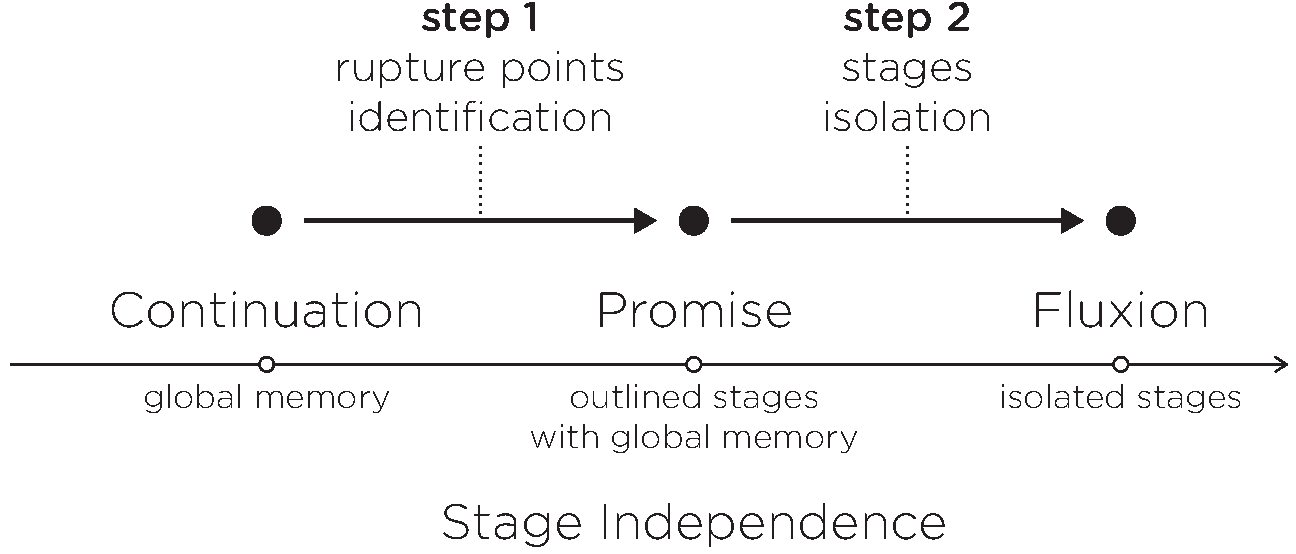
\includegraphics[width=0.7\textwidth]{../resources/roadmap.pdf}%
    \caption{Roadmap}%
    \label{fig:roadmap}%
  }%
\end{figure}

The first compiler focuses on the identification of simple chains of causality between continuations to transform these chains into Promises.
% the transformation from continuations to Promises.
% It focuses on the identification of the chains of causality in continuations.
However, promises are more expressive than the simple chaining of causal sequentiality.
% They force another control over the execution flow.
% According to the outcome of the operation, they call one function to continue the execution with the result, or another to handle errors.
% This conditional execution is indivisible from the Promise specification.
% Promises impose a convention on how to hand back the outcome of the deferred computation, while classic continuations leave this conditional execution to the developer.
Moreover, they impose a different convention than continuations on how to hand back the outcome and errors of the deferred computation.
This difference brings unnecessary complexity to the identification of chains.
To rule out this difference between continuations and Promises, before introducing the first compiler, section \ref{chapter5:due} introduces a simpler specification to Promise, called Due.

The second compiler detects all the chains of causality between continuations and encapsulate them in fluxions.
It isolates the fluxions when possible to allow the parallelism required for efficiency.
This second compilers is introduced in section \ref{chapter5:flx}.

\renewcommand{\glyph}{\iconfont{\XeTeXglyph287}}
\chapter{Implementations} \label{chapter5}
\minitoc
\eject
The transformation allowed by the equivalence from an event-driven program into a distributed network of fluxions is implemented incrementally into two compilers, as presented in figure \ref{fig:roadmap}.
Each compilers is divided into two steps, the identification of the rupture points separating the stages of the pipeline, and the isolation of these stages.
% This chapter presents the technical implementations of these two steps in the transformation from the event-driven execution model to the pipeline architecture
% , the transformation described in the previous chapter was implemented incrementally in two compilers.

\begin{figure}[h!]%
  \textfig{%
    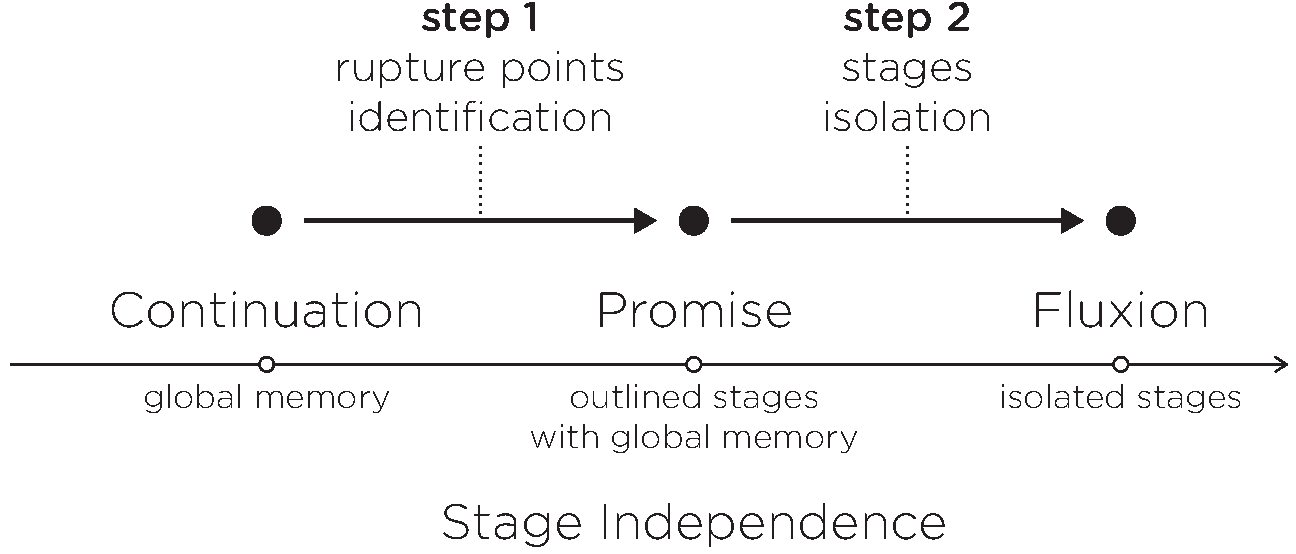
\includegraphics[width=0.7\textwidth]{../resources/roadmap.pdf}%
    \caption{Roadmap}%
    \label{fig:roadmap}%
  }%
\end{figure}

The first compiler focuses on the identification of simple chains of causality between continuations to transform these chains into Promises.
% the transformation from continuations to Promises.
% It focuses on the identification of the chains of causality in continuations.
However, promises are more expressive than the simple chaining of causal sequentiality.
% They force another control over the execution flow.
% According to the outcome of the operation, they call one function to continue the execution with the result, or another to handle errors.
% This conditional execution is indivisible from the Promise specification.
% Promises impose a convention on how to hand back the outcome of the deferred computation, while classic continuations leave this conditional execution to the developer.
Moreover, they impose a different convention than continuations on how to hand back the outcome and errors of the deferred computation.
This difference brings unnecessary complexity to the identification of chains.
To rule out this difference between continuations and Promises, before introducing the first compiler, section \ref{chapter5:due} introduces a simpler specification to Promise, called Due.

The second compiler detects all the chains of causality between continuations and encapsulate them in fluxions.
It isolates the fluxions when possible to allow the parallelism required for efficiency.
This second compilers is introduced in section \ref{chapter5:flx}.

\input{05-implementation/Due/main}
\input{05-implementation/Flx/main}
% \input{05-implementation/Evaluation}

\renewcommand{\glyph}{\iconfont{\XeTeXglyph287}}
\chapter{Implementations} \label{chapter5}
\minitoc
\eject
The transformation allowed by the equivalence from an event-driven program into a distributed network of fluxions is implemented incrementally into two compilers, as presented in figure \ref{fig:roadmap}.
Each compilers is divided into two steps, the identification of the rupture points separating the stages of the pipeline, and the isolation of these stages.
% This chapter presents the technical implementations of these two steps in the transformation from the event-driven execution model to the pipeline architecture
% , the transformation described in the previous chapter was implemented incrementally in two compilers.

\begin{figure}[h!]%
  \textfig{%
    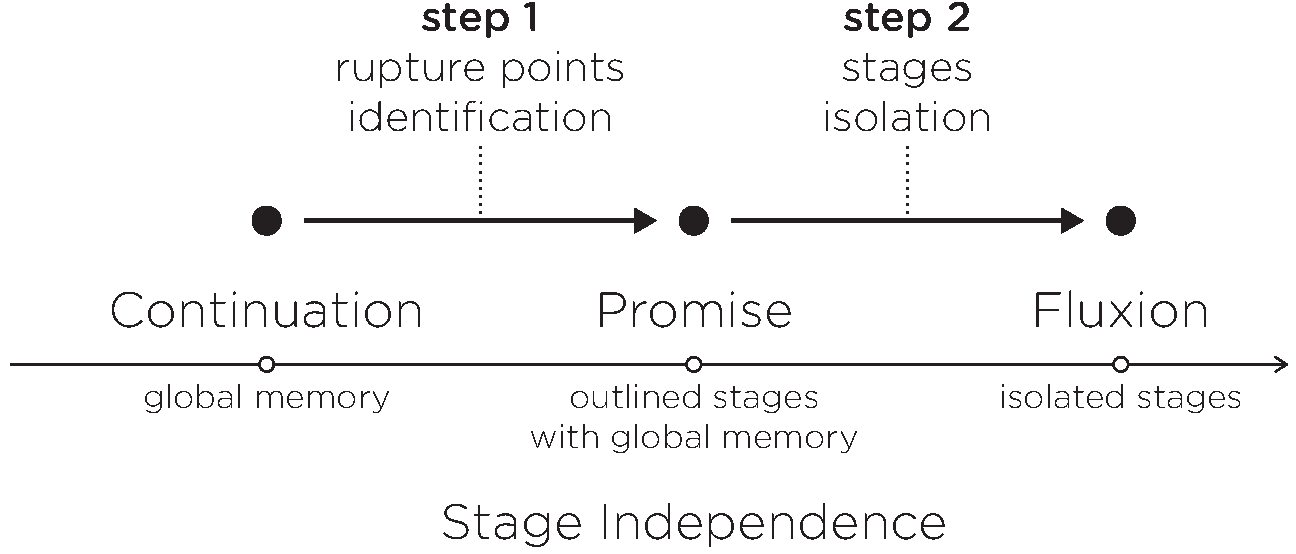
\includegraphics[width=0.7\textwidth]{../resources/roadmap.pdf}%
    \caption{Roadmap}%
    \label{fig:roadmap}%
  }%
\end{figure}

The first compiler focuses on the identification of simple chains of causality between continuations to transform these chains into Promises.
% the transformation from continuations to Promises.
% It focuses on the identification of the chains of causality in continuations.
However, promises are more expressive than the simple chaining of causal sequentiality.
% They force another control over the execution flow.
% According to the outcome of the operation, they call one function to continue the execution with the result, or another to handle errors.
% This conditional execution is indivisible from the Promise specification.
% Promises impose a convention on how to hand back the outcome of the deferred computation, while classic continuations leave this conditional execution to the developer.
Moreover, they impose a different convention than continuations on how to hand back the outcome and errors of the deferred computation.
This difference brings unnecessary complexity to the identification of chains.
To rule out this difference between continuations and Promises, before introducing the first compiler, section \ref{chapter5:due} introduces a simpler specification to Promise, called Due.

The second compiler detects all the chains of causality between continuations and encapsulate them in fluxions.
It isolates the fluxions when possible to allow the parallelism required for efficiency.
This second compilers is introduced in section \ref{chapter5:flx}.

\input{05-implementation/Due/main}
\input{05-implementation/Flx/main}
% \input{05-implementation/Evaluation}

% \subsection{Real test case} \label{chapter5:flx:evaluation}

The compiler is tested on a real application, gifsockets-server\ftnt{https://github.com/twolfson/gifsockets-server}.
This test proves the possibility for an application to be compiled into a network of independent parts.
It shows the current limitations of this isolation and the modifications needed on the application to circumvent them.

\begin{code}[js, caption={Simplified version of gifsockets-server},label={lst:gifsocket}]
var express = require('express'),
    app = express(),
    routes = require('gifsockets-middleware'), //@\label{lst:gifsocket:gif-mw}@
    getRawBody = require('raw-body');

function bodyParser(limit) { //@\label{lst:gifsocket:bodyParser}@
  return function saveBody(req, res, next) { //@\label{lst:gifsocket:saveBody}@
    getRawBody(req, { //@\label{lst:gifsocket:getRawBody}@
      expected: req.headers['content-length'],
      limit: limit
    }, function (err, buffer) { //@\label{lst:gifsocket:callback}@
      req.body = buffer;
      next(); //@\label{lst:gifsocket:next}@
    });
  };
}

app.post('/image/text', bodyParser(1 * 1024 * 1024), routes.writeTextToImages); //@\label{lst:gifsocket:app.post}@
app.listen(8000);
\end{code}

This application, simplified in listing \ref{lst:gifsocket}, is a real-time chat using gif-based communication channels.
It was selected from the evaluation set of the Due compiler because it is simple enough to illustrate this evaluation.
% \cite{Brodu2015}
%  from the \texttt{npm} registry because it depends on \texttt{express}, it is tested, working, and simple enough to illustrate this evaluation.
The server transforms the received text into a gif frame, and pushes it back to a never-ending gif to be displayed on the client.

On line \ref{lst:gifsocket:app.post}, the application registers two functions to process the requests received on the url \texttt{/image/text}.
The closure \texttt{saveBody}, line \ref{lst:gifsocket:saveBody}, returned by \texttt{bodyParser}, line \ref{lst:gifsocket:bodyParser}, and the method \texttt{routes.write\-Text\-To\-Images} from the external module \texttt{gifsockets-\-middleware}, line \ref{lst:gifsocket:gif-mw}.
The closure \texttt{saveBody} calls the asynchronous function \texttt{getRawBody} to get the request body.
Its callback handles the errors, and calls \texttt{next} to continue processing the request with the next function, \texttt{routes.write\-Text\-To\-Images}.

\subsubsection{Compilation} \label{chapter5:flx:evaluation:compilation}

% We compile this application with the compiler
The compilation result is in listing \ref{lst:flx-gifsocket}.
The function call \texttt{app.post}, line \ref{lst:gifsocket:app.post}, is a rupture point.
However, its callbacks, \texttt{bodyParser} and \texttt{routes.write\-Text\-To\-Images} are not declared \textit{in situ}.
They are evaluated as functions only at runtime.
As precised previously, the compiler discards these callbacks to avoid altering the semantic. % by moving or modifying their definition.
% For this reason, the compiler ignores this rupture point, to avoid interfering with the evaluation.

\begin{code}[flx, caption={Compilation result of gifsockets-server},label={lst:flx-gifsocket}]
flx main & express {req}
>> anonymous_1000 [req, next]
  var express = require('express'),
      app = express(),
      routes = require('gifsockets-middleware'), //@\label{lst:flx-gifsocket:gif-mw}@
      getRawBody = require('raw-body');

  function bodyParser(limit) { //@\label{lst:flx-gifsocket:bodyParser}@
    return function saveBody(req, res, next) { //@\label{lst:flx-gifsocket:saveBody}@
      getRawBody(req, { //@\label{lst:flx-gifsocket:getRawBody}@
        expected: req.headers['content-length'], //@\label{lst:flx-gifsocket:req.headers}@
        limit: limit
      }, >> anonymous_1000 [req, next]);
    };
  }

  app.post('/image/text', bodyParser(1 * 1024 * 1024), routes.writeTextToImages); //@\label{lst:flx-gifsocket:app.post}@
  app.listen(8000);

flx anonymous_1000
-> null
  function (err, buffer) { //@\label{lst:flx-gifsocket:callback}@
    req.body = buffer; //@\label{lst:flx-gifsocket:buffer}@
    next(); //@\label{lst:flx-gifsocket:next}@
  }
\end{code}

The compiler detects a rupture point : the function \texttt{get\-Raw\-Body} and its anonymous callback, line \ref{lst:gifsocket:callback}.
It encapsulates this callback in a fluxion named \texttt{anony\-mous\_\-1000}.
The callback is replaced with a stream placeholder to send the message stream to this downstream fluxion.
The variables \texttt{req} and \texttt{next} are appended to this message stream, to propagate their value from the \texttt{main} fluxion to the \texttt{anony\-mous\_\-1000} fluxion.

When \texttt{anony\-mous\_\-1000} is not isolated from the \texttt{main} fluxion, as if they belong to the same group, the compilation result works as expected.
The variables used in the fluxion, \texttt{req} and \texttt{next}, are still shared between the two fluxions.
In this situation fluxions are quite similar to Dues regarding memory shareing.
Our goal is to isolate the two fluxions, to be able to safely parallelize their executions.

\subsubsection{Isolation} \label{chapter5:flx:evaluation:isolation}

In listing \ref{lst:flx-gifsocket}, the fluxion \texttt{anony\-mous\_\-1000} modifies the object \texttt{req}, line \ref{lst:flx-gifsocket:buffer}, to store the text of the received request, and it calls \texttt{next} to continue the execution, line \ref{lst:flx-gifsocket:next}.
\texttt{req} is an alias to a memory location used in multiple palces in code.
Therefore, these operations produce side-effects that should propagate in the whole application, but the isolation prevents this propagation.
Isolating the fluxion \texttt{anony\-mous\_\-1000} produces runtime exceptions.
The next paragraph details how this situation is handled to allow the application to be parallelized.

\paragraph{Variable \texttt{req}}

The variable \texttt{req} is read in fluxion \texttt{main}, lines \ref{lst:flx-gifsocket:getRawBody} and \ref{lst:flx-gifsocket:req.headers}.
Then its property \texttt{body} is associated to \texttt{buffer} in fluxion \texttt{anony\-mous\_\-1000}, line \ref{lst:flx-gifsocket:buffer}.
The compiler is unable to identify the aliases of this variable. % further usages.
However, the side effect resulting from this association impacts a variable in the scope of the next callback, \texttt{routes.write\-Text\-To\-Images}.
In this test case, the application is modified manually to explicitly propagate this side-effect to the next callback through the function \texttt{next}.
The modifications of this function are explained further in the next paragraph.

\paragraph{Closure \texttt{next}}

The function \texttt{next} is a closure provided by the \texttt{express} \texttt{Router} to continue the execution with the next function to handle the client request.
Because it indirectly relies on the variable \texttt{req}, it is impossible to isolate its execution with the \texttt{anony\-mous\_\-1000} fluxion.
Instead, we modify \texttt{express}, so as to be compatible with the fluxional execution model.
We explain the modifications below.

\begin{code}[flx, caption={Simplified modification on the compiled result},label={lst:mflx-gifsocket}]
flx anonymous_1000
-> express_dispatcher
  function (err, buffer) { //@\label{lst:mflx-gifsocket:callback}@
    req.body = buffer; //@\label{lst:mflx-gifsocket:buffer}@
    next_placeholder(req, -> express_dispatcher); //@\label{lst:mflx-gifsocket:next-placeholder}@
  }

flx express_dispatcher & express {req} //@\label{lst:mflx-gifsocket:express-dispatcher}@
-> null
  function (modified_req) {
    merge(req, modified_req);
    next(); //@\label{lst:mflx-gifsocket:next}@
  }
\end{code}

In listing \ref{lst:gifsocket}, the function \texttt{next} is a continuation allowing the anonymous callback, line \ref{lst:gifsocket:callback}, to call the next function to handle the request.
To isolate the anonymous callback into \texttt{anonymous\_\-1000}, \texttt{next} is replaced by a rupture point.
This replacement is illustrated in listing \ref{lst:mflx-gifsocket}.
The \texttt{express} \texttt{Router} registers a fluxion named \texttt{express\_\-dispatcher}, line \ref{lst:mflx-gifsocket:express-dispatcher}, to continue the execution after the fluxion \texttt{anony\-mous\_\-1000}.
This fluxion is in the same group \texttt{express} as the \texttt{main} fluxion, hence it has access to the original variable \texttt{req}, and to the original function \texttt{next}.
The call to the original \texttt{next} function is replaced by a placeholder to push the stream to the fluxion \texttt{express\_\-dispatcher}, line \ref{lst:mflx-gifsocket:next-placeholder}.
The fluxion \texttt{express\_\-dispatcher} receives the stream from the upstream fluxion \texttt{anony\-mous\_\-1000}, merges back the modification in the variable \texttt{req} to propagate the side effects, and finally calls the original function \texttt{next} to continue the execution, line \ref{lst:mflx-gifsocket:next}.

After the modifications detailed above, the server works as expected.
The isolated fluxion correctly receives, and returns its serialized messages.
The client successfully receives a gif frame containing the text.



\subsection{Limitations}

The static analysis used for this compiler presents some limitations.
It is unable to analyze code with dynamic behaviors.
Higher-order programming leads to more productivity partly beacuse it rely on such dynamic behavior to extend expressivity.
Precisely, it allows more levels of indirections.

\subsubsection{Levels of Indirections}

The indirection is an abstraction between the value, and its manipulation.
In listing \ref{lst:indirection}, the variables \texttt{a} and \texttt{b} point both to the same memory object.
The function \texttt{fn} introduces a level of indirection between the real object \texttt{a} and its manipulation handle, \texttt{b};
% Actually, the variable \texttt{a} already introduces a level of indirection between the real object and the handle \texttt{a}.

\begin{code}[js,
  caption={One level of Indirection},
  label={lst:indirection}]
var a = {
      // an object;
    };

fn(b) {
  // modify b;
}

fn(a);
\end{code}

\subsubsection{Uncertainties}

The indirection is trivial to resolve in listing \ref{lst:indirection}.
It only needs to have access to the definition of \texttt{a} and of \texttt{fn}.
%A very simple static analysis could resolve it.
However, in listing \ref{lst:indirections}, the array \texttt{handlers} introduces a new level of indirection.
The static analysis now needs to have access to the definition of \texttt{i} and of the \texttt{handlers}.
If this definition is provided by an external input, it is not available statically, hence, it adds an uncertainty during the analysis. 

\begin{code}[js,
  caption={Two levels of indirection},
  label={lst:indirections}]
var a = {
      // an object;
    },
    handlers = [
      // definition of fn handlers;
    ],
    i = ?;

handlers[i](a);
handlers[i+1](a);
\end{code}

These examples are extremely simplified.
A real application contains enough indirections for the static analysis to be overwhelmed by uncertainties, and to be unable to resolve the variables.
If a variable is left unresolved, it is impossible to assure its scope and its aliases.
Therefore, the compiler is unable to isolate it into a fluxion, or to distribute its modification by messages.

Moreover, it leads the compiler to ignore the rupture points not defined \textit{in situ}, because their modifications could impact the semantic.
The reason for this precaution, is that the compiler is unable to assure where the function is used, and the scope of its variables.
Therefore, it is unable to assure that the modification will conserve the semantic.

\subsubsection{Dynamic Resolution}

In a web application, this variable \texttt{i} might be part of the user request, which is available only at runtime.
It eventually introduces an uncertainty.

This dynamic resolution of variables is precisely what increase expressiveness.
Trying to resolve them statically is equivalent to restrict expressiveness.
No static analysis can overstep these limitations.
Only a dynamic analysis could analysis the resolved indirections during run time to overstep these limitations correctly.




% \subsection{Real test case} \label{chapter5:flx:evaluation}

The compiler is tested on a real application, gifsockets-server\ftnt{https://github.com/twolfson/gifsockets-server}.
This test proves the possibility for an application to be compiled into a network of independent parts.
It shows the current limitations of this isolation and the modifications needed on the application to circumvent them.

\begin{code}[js, caption={Simplified version of gifsockets-server},label={lst:gifsocket}]
var express = require('express'),
    app = express(),
    routes = require('gifsockets-middleware'), //@\label{lst:gifsocket:gif-mw}@
    getRawBody = require('raw-body');

function bodyParser(limit) { //@\label{lst:gifsocket:bodyParser}@
  return function saveBody(req, res, next) { //@\label{lst:gifsocket:saveBody}@
    getRawBody(req, { //@\label{lst:gifsocket:getRawBody}@
      expected: req.headers['content-length'],
      limit: limit
    }, function (err, buffer) { //@\label{lst:gifsocket:callback}@
      req.body = buffer;
      next(); //@\label{lst:gifsocket:next}@
    });
  };
}

app.post('/image/text', bodyParser(1 * 1024 * 1024), routes.writeTextToImages); //@\label{lst:gifsocket:app.post}@
app.listen(8000);
\end{code}

This application, simplified in listing \ref{lst:gifsocket}, is a real-time chat using gif-based communication channels.
It was selected from the evaluation set of the Due compiler because it is simple enough to illustrate this evaluation.
% \cite{Brodu2015}
%  from the \texttt{npm} registry because it depends on \texttt{express}, it is tested, working, and simple enough to illustrate this evaluation.
The server transforms the received text into a gif frame, and pushes it back to a never-ending gif to be displayed on the client.

On line \ref{lst:gifsocket:app.post}, the application registers two functions to process the requests received on the url \texttt{/image/text}.
The closure \texttt{saveBody}, line \ref{lst:gifsocket:saveBody}, returned by \texttt{bodyParser}, line \ref{lst:gifsocket:bodyParser}, and the method \texttt{routes.write\-Text\-To\-Images} from the external module \texttt{gifsockets-\-middleware}, line \ref{lst:gifsocket:gif-mw}.
The closure \texttt{saveBody} calls the asynchronous function \texttt{getRawBody} to get the request body.
Its callback handles the errors, and calls \texttt{next} to continue processing the request with the next function, \texttt{routes.write\-Text\-To\-Images}.

\subsubsection{Compilation} \label{chapter5:flx:evaluation:compilation}

% We compile this application with the compiler
The compilation result is in listing \ref{lst:flx-gifsocket}.
The function call \texttt{app.post}, line \ref{lst:gifsocket:app.post}, is a rupture point.
However, its callbacks, \texttt{bodyParser} and \texttt{routes.write\-Text\-To\-Images} are not declared \textit{in situ}.
They are evaluated as functions only at runtime.
As precised previously, the compiler discards these callbacks to avoid altering the semantic. % by moving or modifying their definition.
% For this reason, the compiler ignores this rupture point, to avoid interfering with the evaluation.

\begin{code}[flx, caption={Compilation result of gifsockets-server},label={lst:flx-gifsocket}]
flx main & express {req}
>> anonymous_1000 [req, next]
  var express = require('express'),
      app = express(),
      routes = require('gifsockets-middleware'), //@\label{lst:flx-gifsocket:gif-mw}@
      getRawBody = require('raw-body');

  function bodyParser(limit) { //@\label{lst:flx-gifsocket:bodyParser}@
    return function saveBody(req, res, next) { //@\label{lst:flx-gifsocket:saveBody}@
      getRawBody(req, { //@\label{lst:flx-gifsocket:getRawBody}@
        expected: req.headers['content-length'], //@\label{lst:flx-gifsocket:req.headers}@
        limit: limit
      }, >> anonymous_1000 [req, next]);
    };
  }

  app.post('/image/text', bodyParser(1 * 1024 * 1024), routes.writeTextToImages); //@\label{lst:flx-gifsocket:app.post}@
  app.listen(8000);

flx anonymous_1000
-> null
  function (err, buffer) { //@\label{lst:flx-gifsocket:callback}@
    req.body = buffer; //@\label{lst:flx-gifsocket:buffer}@
    next(); //@\label{lst:flx-gifsocket:next}@
  }
\end{code}

The compiler detects a rupture point : the function \texttt{get\-Raw\-Body} and its anonymous callback, line \ref{lst:gifsocket:callback}.
It encapsulates this callback in a fluxion named \texttt{anony\-mous\_\-1000}.
The callback is replaced with a stream placeholder to send the message stream to this downstream fluxion.
The variables \texttt{req} and \texttt{next} are appended to this message stream, to propagate their value from the \texttt{main} fluxion to the \texttt{anony\-mous\_\-1000} fluxion.

When \texttt{anony\-mous\_\-1000} is not isolated from the \texttt{main} fluxion, as if they belong to the same group, the compilation result works as expected.
The variables used in the fluxion, \texttt{req} and \texttt{next}, are still shared between the two fluxions.
In this situation fluxions are quite similar to Dues regarding memory shareing.
Our goal is to isolate the two fluxions, to be able to safely parallelize their executions.

\subsubsection{Isolation} \label{chapter5:flx:evaluation:isolation}

In listing \ref{lst:flx-gifsocket}, the fluxion \texttt{anony\-mous\_\-1000} modifies the object \texttt{req}, line \ref{lst:flx-gifsocket:buffer}, to store the text of the received request, and it calls \texttt{next} to continue the execution, line \ref{lst:flx-gifsocket:next}.
\texttt{req} is an alias to a memory location used in multiple palces in code.
Therefore, these operations produce side-effects that should propagate in the whole application, but the isolation prevents this propagation.
Isolating the fluxion \texttt{anony\-mous\_\-1000} produces runtime exceptions.
The next paragraph details how this situation is handled to allow the application to be parallelized.

\paragraph{Variable \texttt{req}}

The variable \texttt{req} is read in fluxion \texttt{main}, lines \ref{lst:flx-gifsocket:getRawBody} and \ref{lst:flx-gifsocket:req.headers}.
Then its property \texttt{body} is associated to \texttt{buffer} in fluxion \texttt{anony\-mous\_\-1000}, line \ref{lst:flx-gifsocket:buffer}.
The compiler is unable to identify the aliases of this variable. % further usages.
However, the side effect resulting from this association impacts a variable in the scope of the next callback, \texttt{routes.write\-Text\-To\-Images}.
In this test case, the application is modified manually to explicitly propagate this side-effect to the next callback through the function \texttt{next}.
The modifications of this function are explained further in the next paragraph.

\paragraph{Closure \texttt{next}}

The function \texttt{next} is a closure provided by the \texttt{express} \texttt{Router} to continue the execution with the next function to handle the client request.
Because it indirectly relies on the variable \texttt{req}, it is impossible to isolate its execution with the \texttt{anony\-mous\_\-1000} fluxion.
Instead, we modify \texttt{express}, so as to be compatible with the fluxional execution model.
We explain the modifications below.

\begin{code}[flx, caption={Simplified modification on the compiled result},label={lst:mflx-gifsocket}]
flx anonymous_1000
-> express_dispatcher
  function (err, buffer) { //@\label{lst:mflx-gifsocket:callback}@
    req.body = buffer; //@\label{lst:mflx-gifsocket:buffer}@
    next_placeholder(req, -> express_dispatcher); //@\label{lst:mflx-gifsocket:next-placeholder}@
  }

flx express_dispatcher & express {req} //@\label{lst:mflx-gifsocket:express-dispatcher}@
-> null
  function (modified_req) {
    merge(req, modified_req);
    next(); //@\label{lst:mflx-gifsocket:next}@
  }
\end{code}

In listing \ref{lst:gifsocket}, the function \texttt{next} is a continuation allowing the anonymous callback, line \ref{lst:gifsocket:callback}, to call the next function to handle the request.
To isolate the anonymous callback into \texttt{anonymous\_\-1000}, \texttt{next} is replaced by a rupture point.
This replacement is illustrated in listing \ref{lst:mflx-gifsocket}.
The \texttt{express} \texttt{Router} registers a fluxion named \texttt{express\_\-dispatcher}, line \ref{lst:mflx-gifsocket:express-dispatcher}, to continue the execution after the fluxion \texttt{anony\-mous\_\-1000}.
This fluxion is in the same group \texttt{express} as the \texttt{main} fluxion, hence it has access to the original variable \texttt{req}, and to the original function \texttt{next}.
The call to the original \texttt{next} function is replaced by a placeholder to push the stream to the fluxion \texttt{express\_\-dispatcher}, line \ref{lst:mflx-gifsocket:next-placeholder}.
The fluxion \texttt{express\_\-dispatcher} receives the stream from the upstream fluxion \texttt{anony\-mous\_\-1000}, merges back the modification in the variable \texttt{req} to propagate the side effects, and finally calls the original function \texttt{next} to continue the execution, line \ref{lst:mflx-gifsocket:next}.

After the modifications detailed above, the server works as expected.
The isolated fluxion correctly receives, and returns its serialized messages.
The client successfully receives a gif frame containing the text.



\subsection{Limitations}

The static analysis used for this compiler presents some limitations.
It is unable to analyze code with dynamic behaviors.
Higher-order programming leads to more productivity partly beacuse it rely on such dynamic behavior to extend expressivity.
Precisely, it allows more levels of indirections.

\subsubsection{Levels of Indirections}

The indirection is an abstraction between the value, and its manipulation.
In listing \ref{lst:indirection}, the variables \texttt{a} and \texttt{b} point both to the same memory object.
The function \texttt{fn} introduces a level of indirection between the real object \texttt{a} and its manipulation handle, \texttt{b};
% Actually, the variable \texttt{a} already introduces a level of indirection between the real object and the handle \texttt{a}.

\begin{code}[js,
  caption={One level of Indirection},
  label={lst:indirection}]
var a = {
      // an object;
    };

fn(b) {
  // modify b;
}

fn(a);
\end{code}

\subsubsection{Uncertainties}

The indirection is trivial to resolve in listing \ref{lst:indirection}.
It only needs to have access to the definition of \texttt{a} and of \texttt{fn}.
%A very simple static analysis could resolve it.
However, in listing \ref{lst:indirections}, the array \texttt{handlers} introduces a new level of indirection.
The static analysis now needs to have access to the definition of \texttt{i} and of the \texttt{handlers}.
If this definition is provided by an external input, it is not available statically, hence, it adds an uncertainty during the analysis. 

\begin{code}[js,
  caption={Two levels of indirection},
  label={lst:indirections}]
var a = {
      // an object;
    },
    handlers = [
      // definition of fn handlers;
    ],
    i = ?;

handlers[i](a);
handlers[i+1](a);
\end{code}

These examples are extremely simplified.
A real application contains enough indirections for the static analysis to be overwhelmed by uncertainties, and to be unable to resolve the variables.
If a variable is left unresolved, it is impossible to assure its scope and its aliases.
Therefore, the compiler is unable to isolate it into a fluxion, or to distribute its modification by messages.

Moreover, it leads the compiler to ignore the rupture points not defined \textit{in situ}, because their modifications could impact the semantic.
The reason for this precaution, is that the compiler is unable to assure where the function is used, and the scope of its variables.
Therefore, it is unable to assure that the modification will conserve the semantic.

\subsubsection{Dynamic Resolution}

In a web application, this variable \texttt{i} might be part of the user request, which is available only at runtime.
It eventually introduces an uncertainty.

This dynamic resolution of variables is precisely what increase expressiveness.
Trying to resolve them statically is equivalent to restrict expressiveness.
No static analysis can overstep these limitations.
Only a dynamic analysis could analysis the resolved indirections during run time to overstep these limitations correctly.





\tableofcontents

\renewcommand{\glyph}{\iconfont{\XeTeXglyph287}}
\chapter{Implementations} \label{chapter5}
\minitoc
\eject
The transformation allowed by the equivalence from an event-driven program into a distributed network of fluxions is implemented incrementally into two compilers, as presented in figure \ref{fig:roadmap}.
Each compilers is divided into two steps, the identification of the rupture points separating the stages of the pipeline, and the isolation of these stages.
% This chapter presents the technical implementations of these two steps in the transformation from the event-driven execution model to the pipeline architecture
% , the transformation described in the previous chapter was implemented incrementally in two compilers.

\begin{figure}[h!]%
  \textfig{%
    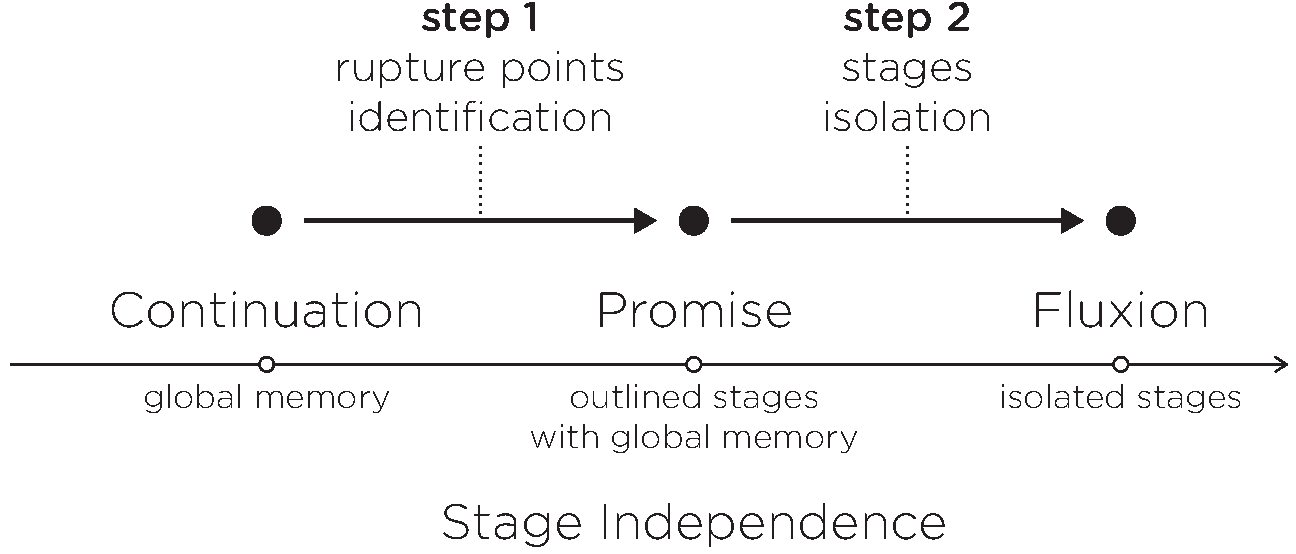
\includegraphics[width=0.7\textwidth]{../resources/roadmap.pdf}%
    \caption{Roadmap}%
    \label{fig:roadmap}%
  }%
\end{figure}

The first compiler focuses on the identification of simple chains of causality between continuations to transform these chains into Promises.
% the transformation from continuations to Promises.
% It focuses on the identification of the chains of causality in continuations.
However, promises are more expressive than the simple chaining of causal sequentiality.
% They force another control over the execution flow.
% According to the outcome of the operation, they call one function to continue the execution with the result, or another to handle errors.
% This conditional execution is indivisible from the Promise specification.
% Promises impose a convention on how to hand back the outcome of the deferred computation, while classic continuations leave this conditional execution to the developer.
Moreover, they impose a different convention than continuations on how to hand back the outcome and errors of the deferred computation.
This difference brings unnecessary complexity to the identification of chains.
To rule out this difference between continuations and Promises, before introducing the first compiler, section \ref{chapter5:due} introduces a simpler specification to Promise, called Due.

The second compiler detects all the chains of causality between continuations and encapsulate them in fluxions.
It isolates the fluxions when possible to allow the parallelism required for efficiency.
This second compilers is introduced in section \ref{chapter5:flx}.

\renewcommand{\glyph}{\iconfont{\XeTeXglyph287}}
\chapter{Implementations} \label{chapter5}
\minitoc
\eject
The transformation allowed by the equivalence from an event-driven program into a distributed network of fluxions is implemented incrementally into two compilers, as presented in figure \ref{fig:roadmap}.
Each compilers is divided into two steps, the identification of the rupture points separating the stages of the pipeline, and the isolation of these stages.
% This chapter presents the technical implementations of these two steps in the transformation from the event-driven execution model to the pipeline architecture
% , the transformation described in the previous chapter was implemented incrementally in two compilers.

\begin{figure}[h!]%
  \textfig{%
    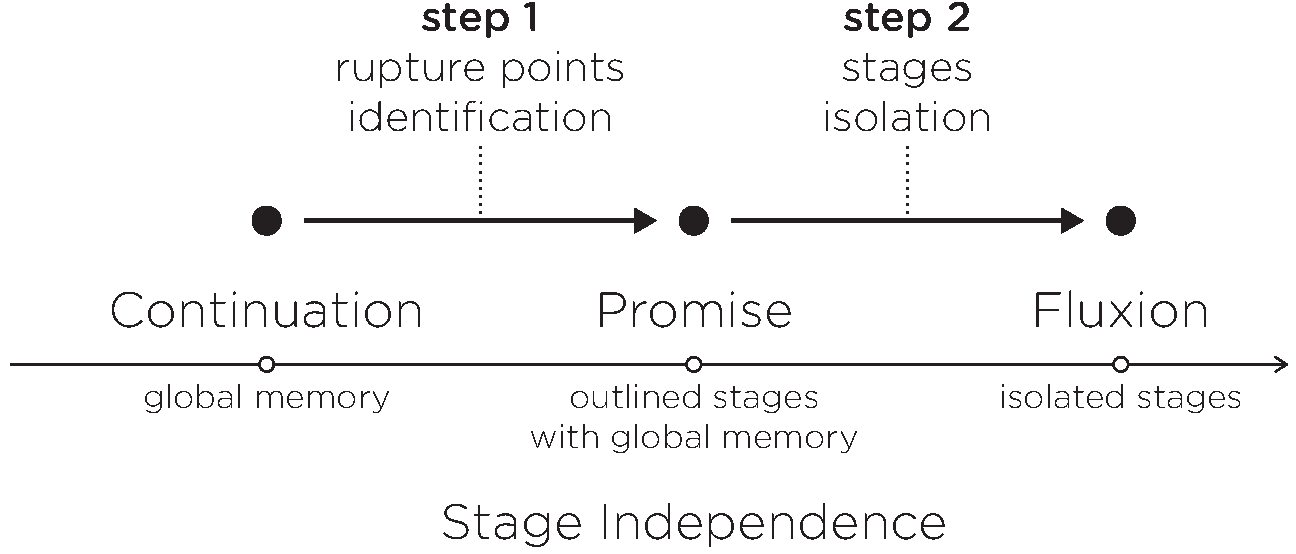
\includegraphics[width=0.7\textwidth]{../resources/roadmap.pdf}%
    \caption{Roadmap}%
    \label{fig:roadmap}%
  }%
\end{figure}

The first compiler focuses on the identification of simple chains of causality between continuations to transform these chains into Promises.
% the transformation from continuations to Promises.
% It focuses on the identification of the chains of causality in continuations.
However, promises are more expressive than the simple chaining of causal sequentiality.
% They force another control over the execution flow.
% According to the outcome of the operation, they call one function to continue the execution with the result, or another to handle errors.
% This conditional execution is indivisible from the Promise specification.
% Promises impose a convention on how to hand back the outcome of the deferred computation, while classic continuations leave this conditional execution to the developer.
Moreover, they impose a different convention than continuations on how to hand back the outcome and errors of the deferred computation.
This difference brings unnecessary complexity to the identification of chains.
To rule out this difference between continuations and Promises, before introducing the first compiler, section \ref{chapter5:due} introduces a simpler specification to Promise, called Due.

The second compiler detects all the chains of causality between continuations and encapsulate them in fluxions.
It isolates the fluxions when possible to allow the parallelism required for efficiency.
This second compilers is introduced in section \ref{chapter5:flx}.

\renewcommand{\glyph}{\iconfont{\XeTeXglyph287}}
\chapter{Implementations} \label{chapter5}
\minitoc
\eject
The transformation allowed by the equivalence from an event-driven program into a distributed network of fluxions is implemented incrementally into two compilers, as presented in figure \ref{fig:roadmap}.
Each compilers is divided into two steps, the identification of the rupture points separating the stages of the pipeline, and the isolation of these stages.
% This chapter presents the technical implementations of these two steps in the transformation from the event-driven execution model to the pipeline architecture
% , the transformation described in the previous chapter was implemented incrementally in two compilers.

\begin{figure}[h!]%
  \textfig{%
    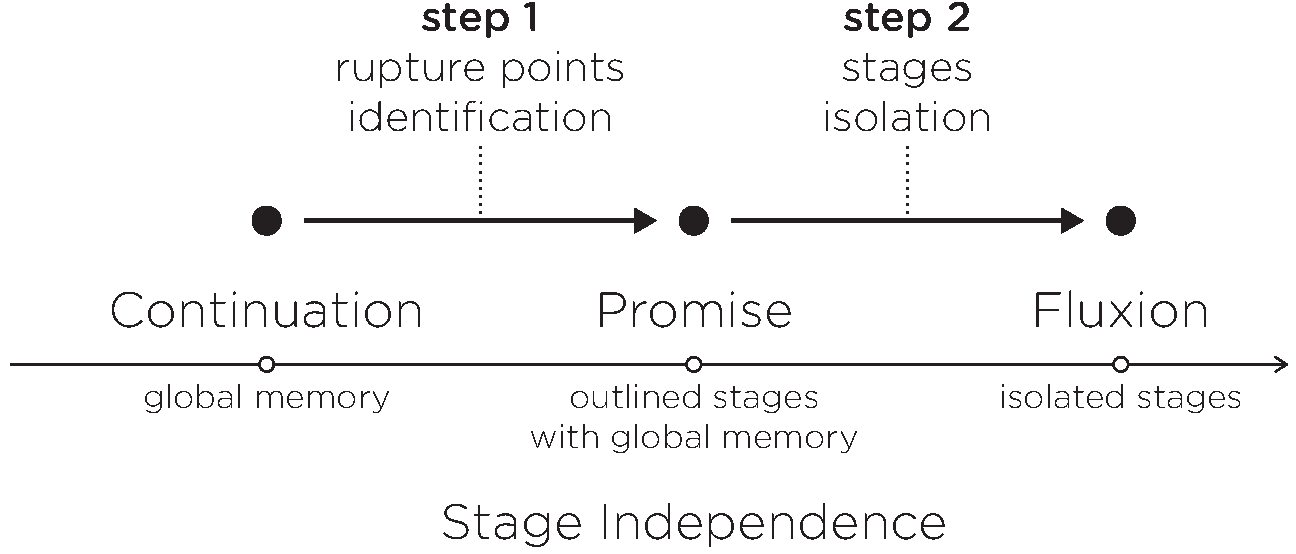
\includegraphics[width=0.7\textwidth]{../resources/roadmap.pdf}%
    \caption{Roadmap}%
    \label{fig:roadmap}%
  }%
\end{figure}

The first compiler focuses on the identification of simple chains of causality between continuations to transform these chains into Promises.
% the transformation from continuations to Promises.
% It focuses on the identification of the chains of causality in continuations.
However, promises are more expressive than the simple chaining of causal sequentiality.
% They force another control over the execution flow.
% According to the outcome of the operation, they call one function to continue the execution with the result, or another to handle errors.
% This conditional execution is indivisible from the Promise specification.
% Promises impose a convention on how to hand back the outcome of the deferred computation, while classic continuations leave this conditional execution to the developer.
Moreover, they impose a different convention than continuations on how to hand back the outcome and errors of the deferred computation.
This difference brings unnecessary complexity to the identification of chains.
To rule out this difference between continuations and Promises, before introducing the first compiler, section \ref{chapter5:due} introduces a simpler specification to Promise, called Due.

The second compiler detects all the chains of causality between continuations and encapsulate them in fluxions.
It isolates the fluxions when possible to allow the parallelism required for efficiency.
This second compilers is introduced in section \ref{chapter5:flx}.

\input{05-implementation/Due/main}
\input{05-implementation/Flx/main}
% \input{05-implementation/Evaluation}

\renewcommand{\glyph}{\iconfont{\XeTeXglyph287}}
\chapter{Implementations} \label{chapter5}
\minitoc
\eject
The transformation allowed by the equivalence from an event-driven program into a distributed network of fluxions is implemented incrementally into two compilers, as presented in figure \ref{fig:roadmap}.
Each compilers is divided into two steps, the identification of the rupture points separating the stages of the pipeline, and the isolation of these stages.
% This chapter presents the technical implementations of these two steps in the transformation from the event-driven execution model to the pipeline architecture
% , the transformation described in the previous chapter was implemented incrementally in two compilers.

\begin{figure}[h!]%
  \textfig{%
    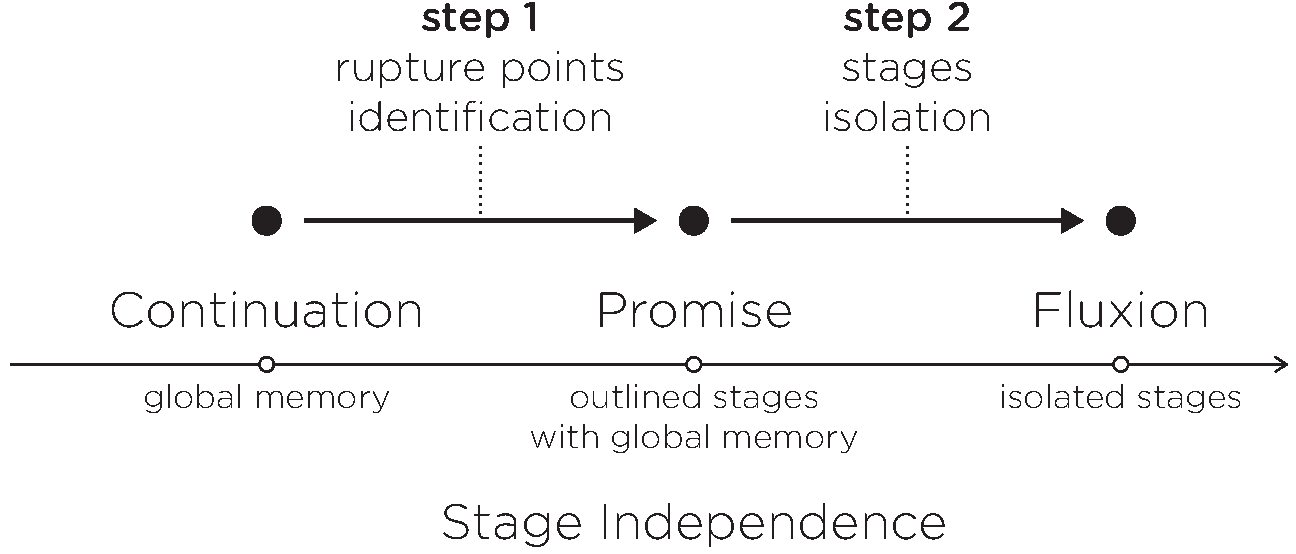
\includegraphics[width=0.7\textwidth]{../resources/roadmap.pdf}%
    \caption{Roadmap}%
    \label{fig:roadmap}%
  }%
\end{figure}

The first compiler focuses on the identification of simple chains of causality between continuations to transform these chains into Promises.
% the transformation from continuations to Promises.
% It focuses on the identification of the chains of causality in continuations.
However, promises are more expressive than the simple chaining of causal sequentiality.
% They force another control over the execution flow.
% According to the outcome of the operation, they call one function to continue the execution with the result, or another to handle errors.
% This conditional execution is indivisible from the Promise specification.
% Promises impose a convention on how to hand back the outcome of the deferred computation, while classic continuations leave this conditional execution to the developer.
Moreover, they impose a different convention than continuations on how to hand back the outcome and errors of the deferred computation.
This difference brings unnecessary complexity to the identification of chains.
To rule out this difference between continuations and Promises, before introducing the first compiler, section \ref{chapter5:due} introduces a simpler specification to Promise, called Due.

The second compiler detects all the chains of causality between continuations and encapsulate them in fluxions.
It isolates the fluxions when possible to allow the parallelism required for efficiency.
This second compilers is introduced in section \ref{chapter5:flx}.

\input{05-implementation/Due/main}
\input{05-implementation/Flx/main}
% \input{05-implementation/Evaluation}

% \subsection{Real test case} \label{chapter5:flx:evaluation}

The compiler is tested on a real application, gifsockets-server\ftnt{https://github.com/twolfson/gifsockets-server}.
This test proves the possibility for an application to be compiled into a network of independent parts.
It shows the current limitations of this isolation and the modifications needed on the application to circumvent them.

\begin{code}[js, caption={Simplified version of gifsockets-server},label={lst:gifsocket}]
var express = require('express'),
    app = express(),
    routes = require('gifsockets-middleware'), //@\label{lst:gifsocket:gif-mw}@
    getRawBody = require('raw-body');

function bodyParser(limit) { //@\label{lst:gifsocket:bodyParser}@
  return function saveBody(req, res, next) { //@\label{lst:gifsocket:saveBody}@
    getRawBody(req, { //@\label{lst:gifsocket:getRawBody}@
      expected: req.headers['content-length'],
      limit: limit
    }, function (err, buffer) { //@\label{lst:gifsocket:callback}@
      req.body = buffer;
      next(); //@\label{lst:gifsocket:next}@
    });
  };
}

app.post('/image/text', bodyParser(1 * 1024 * 1024), routes.writeTextToImages); //@\label{lst:gifsocket:app.post}@
app.listen(8000);
\end{code}

This application, simplified in listing \ref{lst:gifsocket}, is a real-time chat using gif-based communication channels.
It was selected from the evaluation set of the Due compiler because it is simple enough to illustrate this evaluation.
% \cite{Brodu2015}
%  from the \texttt{npm} registry because it depends on \texttt{express}, it is tested, working, and simple enough to illustrate this evaluation.
The server transforms the received text into a gif frame, and pushes it back to a never-ending gif to be displayed on the client.

On line \ref{lst:gifsocket:app.post}, the application registers two functions to process the requests received on the url \texttt{/image/text}.
The closure \texttt{saveBody}, line \ref{lst:gifsocket:saveBody}, returned by \texttt{bodyParser}, line \ref{lst:gifsocket:bodyParser}, and the method \texttt{routes.write\-Text\-To\-Images} from the external module \texttt{gifsockets-\-middleware}, line \ref{lst:gifsocket:gif-mw}.
The closure \texttt{saveBody} calls the asynchronous function \texttt{getRawBody} to get the request body.
Its callback handles the errors, and calls \texttt{next} to continue processing the request with the next function, \texttt{routes.write\-Text\-To\-Images}.

\subsubsection{Compilation} \label{chapter5:flx:evaluation:compilation}

% We compile this application with the compiler
The compilation result is in listing \ref{lst:flx-gifsocket}.
The function call \texttt{app.post}, line \ref{lst:gifsocket:app.post}, is a rupture point.
However, its callbacks, \texttt{bodyParser} and \texttt{routes.write\-Text\-To\-Images} are not declared \textit{in situ}.
They are evaluated as functions only at runtime.
As precised previously, the compiler discards these callbacks to avoid altering the semantic. % by moving or modifying their definition.
% For this reason, the compiler ignores this rupture point, to avoid interfering with the evaluation.

\begin{code}[flx, caption={Compilation result of gifsockets-server},label={lst:flx-gifsocket}]
flx main & express {req}
>> anonymous_1000 [req, next]
  var express = require('express'),
      app = express(),
      routes = require('gifsockets-middleware'), //@\label{lst:flx-gifsocket:gif-mw}@
      getRawBody = require('raw-body');

  function bodyParser(limit) { //@\label{lst:flx-gifsocket:bodyParser}@
    return function saveBody(req, res, next) { //@\label{lst:flx-gifsocket:saveBody}@
      getRawBody(req, { //@\label{lst:flx-gifsocket:getRawBody}@
        expected: req.headers['content-length'], //@\label{lst:flx-gifsocket:req.headers}@
        limit: limit
      }, >> anonymous_1000 [req, next]);
    };
  }

  app.post('/image/text', bodyParser(1 * 1024 * 1024), routes.writeTextToImages); //@\label{lst:flx-gifsocket:app.post}@
  app.listen(8000);

flx anonymous_1000
-> null
  function (err, buffer) { //@\label{lst:flx-gifsocket:callback}@
    req.body = buffer; //@\label{lst:flx-gifsocket:buffer}@
    next(); //@\label{lst:flx-gifsocket:next}@
  }
\end{code}

The compiler detects a rupture point : the function \texttt{get\-Raw\-Body} and its anonymous callback, line \ref{lst:gifsocket:callback}.
It encapsulates this callback in a fluxion named \texttt{anony\-mous\_\-1000}.
The callback is replaced with a stream placeholder to send the message stream to this downstream fluxion.
The variables \texttt{req} and \texttt{next} are appended to this message stream, to propagate their value from the \texttt{main} fluxion to the \texttt{anony\-mous\_\-1000} fluxion.

When \texttt{anony\-mous\_\-1000} is not isolated from the \texttt{main} fluxion, as if they belong to the same group, the compilation result works as expected.
The variables used in the fluxion, \texttt{req} and \texttt{next}, are still shared between the two fluxions.
In this situation fluxions are quite similar to Dues regarding memory shareing.
Our goal is to isolate the two fluxions, to be able to safely parallelize their executions.

\subsubsection{Isolation} \label{chapter5:flx:evaluation:isolation}

In listing \ref{lst:flx-gifsocket}, the fluxion \texttt{anony\-mous\_\-1000} modifies the object \texttt{req}, line \ref{lst:flx-gifsocket:buffer}, to store the text of the received request, and it calls \texttt{next} to continue the execution, line \ref{lst:flx-gifsocket:next}.
\texttt{req} is an alias to a memory location used in multiple palces in code.
Therefore, these operations produce side-effects that should propagate in the whole application, but the isolation prevents this propagation.
Isolating the fluxion \texttt{anony\-mous\_\-1000} produces runtime exceptions.
The next paragraph details how this situation is handled to allow the application to be parallelized.

\paragraph{Variable \texttt{req}}

The variable \texttt{req} is read in fluxion \texttt{main}, lines \ref{lst:flx-gifsocket:getRawBody} and \ref{lst:flx-gifsocket:req.headers}.
Then its property \texttt{body} is associated to \texttt{buffer} in fluxion \texttt{anony\-mous\_\-1000}, line \ref{lst:flx-gifsocket:buffer}.
The compiler is unable to identify the aliases of this variable. % further usages.
However, the side effect resulting from this association impacts a variable in the scope of the next callback, \texttt{routes.write\-Text\-To\-Images}.
In this test case, the application is modified manually to explicitly propagate this side-effect to the next callback through the function \texttt{next}.
The modifications of this function are explained further in the next paragraph.

\paragraph{Closure \texttt{next}}

The function \texttt{next} is a closure provided by the \texttt{express} \texttt{Router} to continue the execution with the next function to handle the client request.
Because it indirectly relies on the variable \texttt{req}, it is impossible to isolate its execution with the \texttt{anony\-mous\_\-1000} fluxion.
Instead, we modify \texttt{express}, so as to be compatible with the fluxional execution model.
We explain the modifications below.

\begin{code}[flx, caption={Simplified modification on the compiled result},label={lst:mflx-gifsocket}]
flx anonymous_1000
-> express_dispatcher
  function (err, buffer) { //@\label{lst:mflx-gifsocket:callback}@
    req.body = buffer; //@\label{lst:mflx-gifsocket:buffer}@
    next_placeholder(req, -> express_dispatcher); //@\label{lst:mflx-gifsocket:next-placeholder}@
  }

flx express_dispatcher & express {req} //@\label{lst:mflx-gifsocket:express-dispatcher}@
-> null
  function (modified_req) {
    merge(req, modified_req);
    next(); //@\label{lst:mflx-gifsocket:next}@
  }
\end{code}

In listing \ref{lst:gifsocket}, the function \texttt{next} is a continuation allowing the anonymous callback, line \ref{lst:gifsocket:callback}, to call the next function to handle the request.
To isolate the anonymous callback into \texttt{anonymous\_\-1000}, \texttt{next} is replaced by a rupture point.
This replacement is illustrated in listing \ref{lst:mflx-gifsocket}.
The \texttt{express} \texttt{Router} registers a fluxion named \texttt{express\_\-dispatcher}, line \ref{lst:mflx-gifsocket:express-dispatcher}, to continue the execution after the fluxion \texttt{anony\-mous\_\-1000}.
This fluxion is in the same group \texttt{express} as the \texttt{main} fluxion, hence it has access to the original variable \texttt{req}, and to the original function \texttt{next}.
The call to the original \texttt{next} function is replaced by a placeholder to push the stream to the fluxion \texttt{express\_\-dispatcher}, line \ref{lst:mflx-gifsocket:next-placeholder}.
The fluxion \texttt{express\_\-dispatcher} receives the stream from the upstream fluxion \texttt{anony\-mous\_\-1000}, merges back the modification in the variable \texttt{req} to propagate the side effects, and finally calls the original function \texttt{next} to continue the execution, line \ref{lst:mflx-gifsocket:next}.

After the modifications detailed above, the server works as expected.
The isolated fluxion correctly receives, and returns its serialized messages.
The client successfully receives a gif frame containing the text.



\subsection{Limitations}

The static analysis used for this compiler presents some limitations.
It is unable to analyze code with dynamic behaviors.
Higher-order programming leads to more productivity partly beacuse it rely on such dynamic behavior to extend expressivity.
Precisely, it allows more levels of indirections.

\subsubsection{Levels of Indirections}

The indirection is an abstraction between the value, and its manipulation.
In listing \ref{lst:indirection}, the variables \texttt{a} and \texttt{b} point both to the same memory object.
The function \texttt{fn} introduces a level of indirection between the real object \texttt{a} and its manipulation handle, \texttt{b};
% Actually, the variable \texttt{a} already introduces a level of indirection between the real object and the handle \texttt{a}.

\begin{code}[js,
  caption={One level of Indirection},
  label={lst:indirection}]
var a = {
      // an object;
    };

fn(b) {
  // modify b;
}

fn(a);
\end{code}

\subsubsection{Uncertainties}

The indirection is trivial to resolve in listing \ref{lst:indirection}.
It only needs to have access to the definition of \texttt{a} and of \texttt{fn}.
%A very simple static analysis could resolve it.
However, in listing \ref{lst:indirections}, the array \texttt{handlers} introduces a new level of indirection.
The static analysis now needs to have access to the definition of \texttt{i} and of the \texttt{handlers}.
If this definition is provided by an external input, it is not available statically, hence, it adds an uncertainty during the analysis. 

\begin{code}[js,
  caption={Two levels of indirection},
  label={lst:indirections}]
var a = {
      // an object;
    },
    handlers = [
      // definition of fn handlers;
    ],
    i = ?;

handlers[i](a);
handlers[i+1](a);
\end{code}

These examples are extremely simplified.
A real application contains enough indirections for the static analysis to be overwhelmed by uncertainties, and to be unable to resolve the variables.
If a variable is left unresolved, it is impossible to assure its scope and its aliases.
Therefore, the compiler is unable to isolate it into a fluxion, or to distribute its modification by messages.

Moreover, it leads the compiler to ignore the rupture points not defined \textit{in situ}, because their modifications could impact the semantic.
The reason for this precaution, is that the compiler is unable to assure where the function is used, and the scope of its variables.
Therefore, it is unable to assure that the modification will conserve the semantic.

\subsubsection{Dynamic Resolution}

In a web application, this variable \texttt{i} might be part of the user request, which is available only at runtime.
It eventually introduces an uncertainty.

This dynamic resolution of variables is precisely what increase expressiveness.
Trying to resolve them statically is equivalent to restrict expressiveness.
No static analysis can overstep these limitations.
Only a dynamic analysis could analysis the resolved indirections during run time to overstep these limitations correctly.




\renewcommand{\glyph}{\iconfont{\XeTeXglyph287}}
\chapter{Implementations} \label{chapter5}
\minitoc
\eject
The transformation allowed by the equivalence from an event-driven program into a distributed network of fluxions is implemented incrementally into two compilers, as presented in figure \ref{fig:roadmap}.
Each compilers is divided into two steps, the identification of the rupture points separating the stages of the pipeline, and the isolation of these stages.
% This chapter presents the technical implementations of these two steps in the transformation from the event-driven execution model to the pipeline architecture
% , the transformation described in the previous chapter was implemented incrementally in two compilers.

\begin{figure}[h!]%
  \textfig{%
    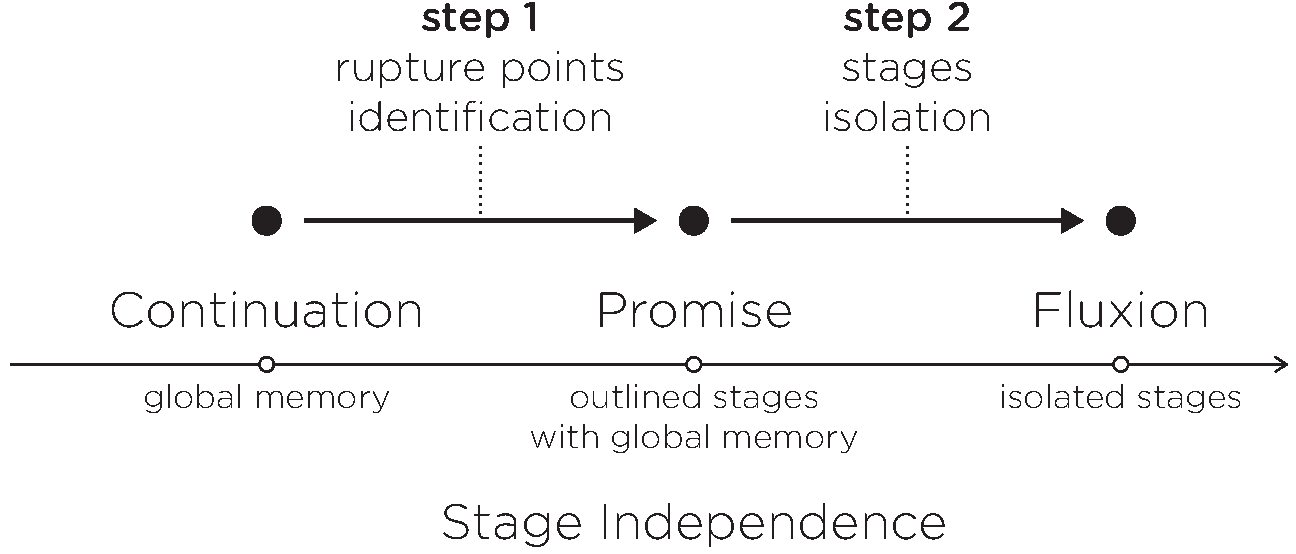
\includegraphics[width=0.7\textwidth]{../resources/roadmap.pdf}%
    \caption{Roadmap}%
    \label{fig:roadmap}%
  }%
\end{figure}

The first compiler focuses on the identification of simple chains of causality between continuations to transform these chains into Promises.
% the transformation from continuations to Promises.
% It focuses on the identification of the chains of causality in continuations.
However, promises are more expressive than the simple chaining of causal sequentiality.
% They force another control over the execution flow.
% According to the outcome of the operation, they call one function to continue the execution with the result, or another to handle errors.
% This conditional execution is indivisible from the Promise specification.
% Promises impose a convention on how to hand back the outcome of the deferred computation, while classic continuations leave this conditional execution to the developer.
Moreover, they impose a different convention than continuations on how to hand back the outcome and errors of the deferred computation.
This difference brings unnecessary complexity to the identification of chains.
To rule out this difference between continuations and Promises, before introducing the first compiler, section \ref{chapter5:due} introduces a simpler specification to Promise, called Due.

The second compiler detects all the chains of causality between continuations and encapsulate them in fluxions.
It isolates the fluxions when possible to allow the parallelism required for efficiency.
This second compilers is introduced in section \ref{chapter5:flx}.

\renewcommand{\glyph}{\iconfont{\XeTeXglyph287}}
\chapter{Implementations} \label{chapter5}
\minitoc
\eject
The transformation allowed by the equivalence from an event-driven program into a distributed network of fluxions is implemented incrementally into two compilers, as presented in figure \ref{fig:roadmap}.
Each compilers is divided into two steps, the identification of the rupture points separating the stages of the pipeline, and the isolation of these stages.
% This chapter presents the technical implementations of these two steps in the transformation from the event-driven execution model to the pipeline architecture
% , the transformation described in the previous chapter was implemented incrementally in two compilers.

\begin{figure}[h!]%
  \textfig{%
    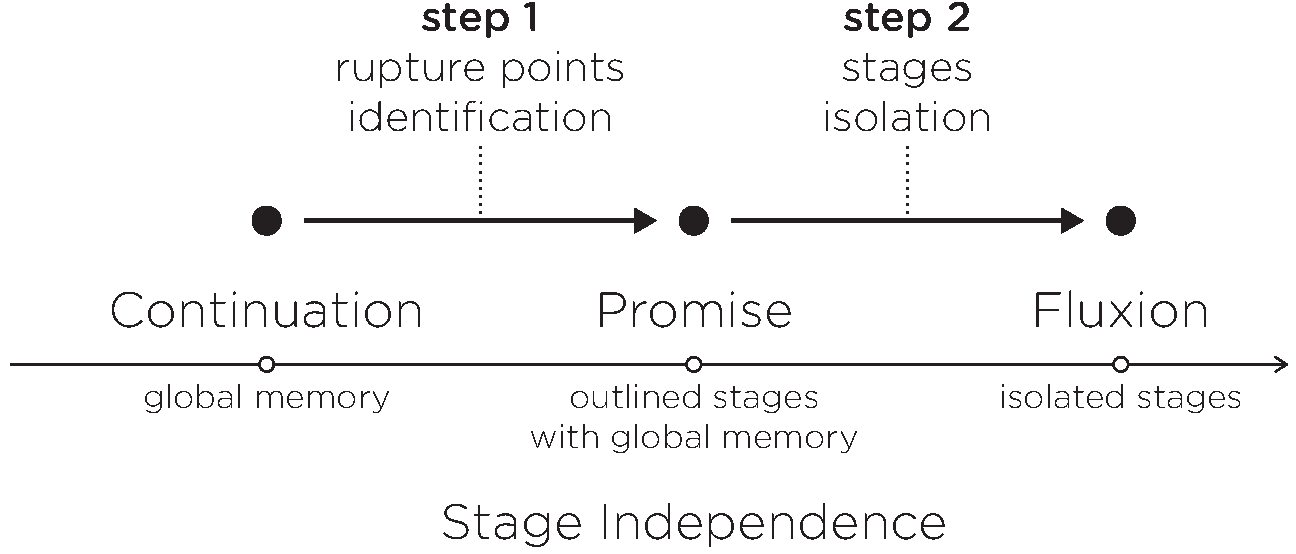
\includegraphics[width=0.7\textwidth]{../resources/roadmap.pdf}%
    \caption{Roadmap}%
    \label{fig:roadmap}%
  }%
\end{figure}

The first compiler focuses on the identification of simple chains of causality between continuations to transform these chains into Promises.
% the transformation from continuations to Promises.
% It focuses on the identification of the chains of causality in continuations.
However, promises are more expressive than the simple chaining of causal sequentiality.
% They force another control over the execution flow.
% According to the outcome of the operation, they call one function to continue the execution with the result, or another to handle errors.
% This conditional execution is indivisible from the Promise specification.
% Promises impose a convention on how to hand back the outcome of the deferred computation, while classic continuations leave this conditional execution to the developer.
Moreover, they impose a different convention than continuations on how to hand back the outcome and errors of the deferred computation.
This difference brings unnecessary complexity to the identification of chains.
To rule out this difference between continuations and Promises, before introducing the first compiler, section \ref{chapter5:due} introduces a simpler specification to Promise, called Due.

The second compiler detects all the chains of causality between continuations and encapsulate them in fluxions.
It isolates the fluxions when possible to allow the parallelism required for efficiency.
This second compilers is introduced in section \ref{chapter5:flx}.

\input{05-implementation/Due/main}
\input{05-implementation/Flx/main}
% \input{05-implementation/Evaluation}

\renewcommand{\glyph}{\iconfont{\XeTeXglyph287}}
\chapter{Implementations} \label{chapter5}
\minitoc
\eject
The transformation allowed by the equivalence from an event-driven program into a distributed network of fluxions is implemented incrementally into two compilers, as presented in figure \ref{fig:roadmap}.
Each compilers is divided into two steps, the identification of the rupture points separating the stages of the pipeline, and the isolation of these stages.
% This chapter presents the technical implementations of these two steps in the transformation from the event-driven execution model to the pipeline architecture
% , the transformation described in the previous chapter was implemented incrementally in two compilers.

\begin{figure}[h!]%
  \textfig{%
    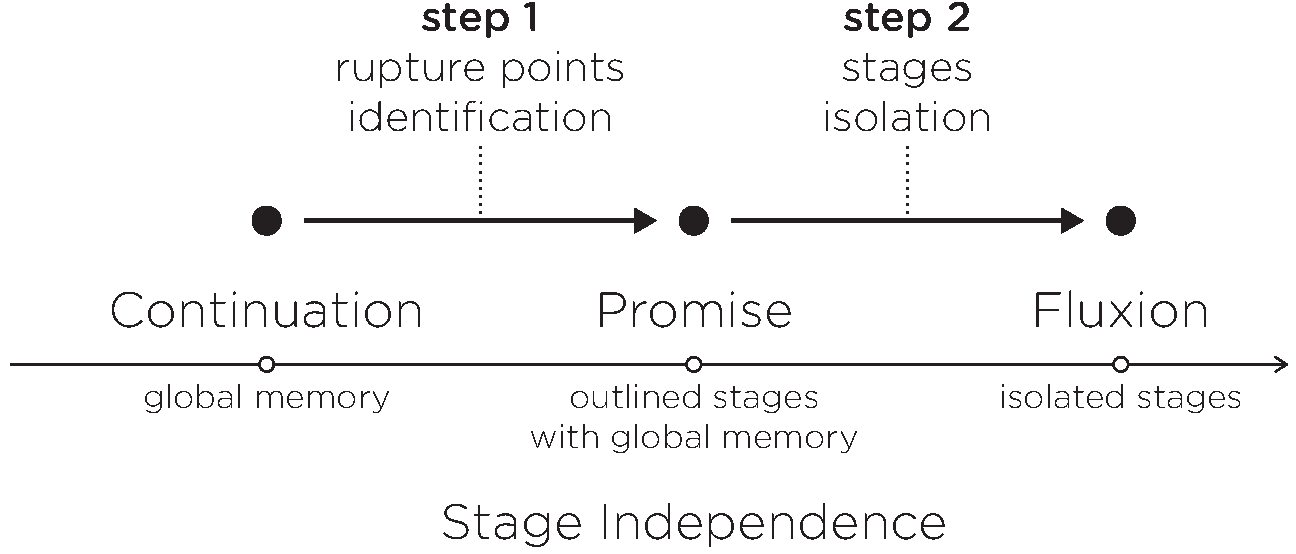
\includegraphics[width=0.7\textwidth]{../resources/roadmap.pdf}%
    \caption{Roadmap}%
    \label{fig:roadmap}%
  }%
\end{figure}

The first compiler focuses on the identification of simple chains of causality between continuations to transform these chains into Promises.
% the transformation from continuations to Promises.
% It focuses on the identification of the chains of causality in continuations.
However, promises are more expressive than the simple chaining of causal sequentiality.
% They force another control over the execution flow.
% According to the outcome of the operation, they call one function to continue the execution with the result, or another to handle errors.
% This conditional execution is indivisible from the Promise specification.
% Promises impose a convention on how to hand back the outcome of the deferred computation, while classic continuations leave this conditional execution to the developer.
Moreover, they impose a different convention than continuations on how to hand back the outcome and errors of the deferred computation.
This difference brings unnecessary complexity to the identification of chains.
To rule out this difference between continuations and Promises, before introducing the first compiler, section \ref{chapter5:due} introduces a simpler specification to Promise, called Due.

The second compiler detects all the chains of causality between continuations and encapsulate them in fluxions.
It isolates the fluxions when possible to allow the parallelism required for efficiency.
This second compilers is introduced in section \ref{chapter5:flx}.

\input{05-implementation/Due/main}
\input{05-implementation/Flx/main}
% \input{05-implementation/Evaluation}

% \subsection{Real test case} \label{chapter5:flx:evaluation}

The compiler is tested on a real application, gifsockets-server\ftnt{https://github.com/twolfson/gifsockets-server}.
This test proves the possibility for an application to be compiled into a network of independent parts.
It shows the current limitations of this isolation and the modifications needed on the application to circumvent them.

\begin{code}[js, caption={Simplified version of gifsockets-server},label={lst:gifsocket}]
var express = require('express'),
    app = express(),
    routes = require('gifsockets-middleware'), //@\label{lst:gifsocket:gif-mw}@
    getRawBody = require('raw-body');

function bodyParser(limit) { //@\label{lst:gifsocket:bodyParser}@
  return function saveBody(req, res, next) { //@\label{lst:gifsocket:saveBody}@
    getRawBody(req, { //@\label{lst:gifsocket:getRawBody}@
      expected: req.headers['content-length'],
      limit: limit
    }, function (err, buffer) { //@\label{lst:gifsocket:callback}@
      req.body = buffer;
      next(); //@\label{lst:gifsocket:next}@
    });
  };
}

app.post('/image/text', bodyParser(1 * 1024 * 1024), routes.writeTextToImages); //@\label{lst:gifsocket:app.post}@
app.listen(8000);
\end{code}

This application, simplified in listing \ref{lst:gifsocket}, is a real-time chat using gif-based communication channels.
It was selected from the evaluation set of the Due compiler because it is simple enough to illustrate this evaluation.
% \cite{Brodu2015}
%  from the \texttt{npm} registry because it depends on \texttt{express}, it is tested, working, and simple enough to illustrate this evaluation.
The server transforms the received text into a gif frame, and pushes it back to a never-ending gif to be displayed on the client.

On line \ref{lst:gifsocket:app.post}, the application registers two functions to process the requests received on the url \texttt{/image/text}.
The closure \texttt{saveBody}, line \ref{lst:gifsocket:saveBody}, returned by \texttt{bodyParser}, line \ref{lst:gifsocket:bodyParser}, and the method \texttt{routes.write\-Text\-To\-Images} from the external module \texttt{gifsockets-\-middleware}, line \ref{lst:gifsocket:gif-mw}.
The closure \texttt{saveBody} calls the asynchronous function \texttt{getRawBody} to get the request body.
Its callback handles the errors, and calls \texttt{next} to continue processing the request with the next function, \texttt{routes.write\-Text\-To\-Images}.

\subsubsection{Compilation} \label{chapter5:flx:evaluation:compilation}

% We compile this application with the compiler
The compilation result is in listing \ref{lst:flx-gifsocket}.
The function call \texttt{app.post}, line \ref{lst:gifsocket:app.post}, is a rupture point.
However, its callbacks, \texttt{bodyParser} and \texttt{routes.write\-Text\-To\-Images} are not declared \textit{in situ}.
They are evaluated as functions only at runtime.
As precised previously, the compiler discards these callbacks to avoid altering the semantic. % by moving or modifying their definition.
% For this reason, the compiler ignores this rupture point, to avoid interfering with the evaluation.

\begin{code}[flx, caption={Compilation result of gifsockets-server},label={lst:flx-gifsocket}]
flx main & express {req}
>> anonymous_1000 [req, next]
  var express = require('express'),
      app = express(),
      routes = require('gifsockets-middleware'), //@\label{lst:flx-gifsocket:gif-mw}@
      getRawBody = require('raw-body');

  function bodyParser(limit) { //@\label{lst:flx-gifsocket:bodyParser}@
    return function saveBody(req, res, next) { //@\label{lst:flx-gifsocket:saveBody}@
      getRawBody(req, { //@\label{lst:flx-gifsocket:getRawBody}@
        expected: req.headers['content-length'], //@\label{lst:flx-gifsocket:req.headers}@
        limit: limit
      }, >> anonymous_1000 [req, next]);
    };
  }

  app.post('/image/text', bodyParser(1 * 1024 * 1024), routes.writeTextToImages); //@\label{lst:flx-gifsocket:app.post}@
  app.listen(8000);

flx anonymous_1000
-> null
  function (err, buffer) { //@\label{lst:flx-gifsocket:callback}@
    req.body = buffer; //@\label{lst:flx-gifsocket:buffer}@
    next(); //@\label{lst:flx-gifsocket:next}@
  }
\end{code}

The compiler detects a rupture point : the function \texttt{get\-Raw\-Body} and its anonymous callback, line \ref{lst:gifsocket:callback}.
It encapsulates this callback in a fluxion named \texttt{anony\-mous\_\-1000}.
The callback is replaced with a stream placeholder to send the message stream to this downstream fluxion.
The variables \texttt{req} and \texttt{next} are appended to this message stream, to propagate their value from the \texttt{main} fluxion to the \texttt{anony\-mous\_\-1000} fluxion.

When \texttt{anony\-mous\_\-1000} is not isolated from the \texttt{main} fluxion, as if they belong to the same group, the compilation result works as expected.
The variables used in the fluxion, \texttt{req} and \texttt{next}, are still shared between the two fluxions.
In this situation fluxions are quite similar to Dues regarding memory shareing.
Our goal is to isolate the two fluxions, to be able to safely parallelize their executions.

\subsubsection{Isolation} \label{chapter5:flx:evaluation:isolation}

In listing \ref{lst:flx-gifsocket}, the fluxion \texttt{anony\-mous\_\-1000} modifies the object \texttt{req}, line \ref{lst:flx-gifsocket:buffer}, to store the text of the received request, and it calls \texttt{next} to continue the execution, line \ref{lst:flx-gifsocket:next}.
\texttt{req} is an alias to a memory location used in multiple palces in code.
Therefore, these operations produce side-effects that should propagate in the whole application, but the isolation prevents this propagation.
Isolating the fluxion \texttt{anony\-mous\_\-1000} produces runtime exceptions.
The next paragraph details how this situation is handled to allow the application to be parallelized.

\paragraph{Variable \texttt{req}}

The variable \texttt{req} is read in fluxion \texttt{main}, lines \ref{lst:flx-gifsocket:getRawBody} and \ref{lst:flx-gifsocket:req.headers}.
Then its property \texttt{body} is associated to \texttt{buffer} in fluxion \texttt{anony\-mous\_\-1000}, line \ref{lst:flx-gifsocket:buffer}.
The compiler is unable to identify the aliases of this variable. % further usages.
However, the side effect resulting from this association impacts a variable in the scope of the next callback, \texttt{routes.write\-Text\-To\-Images}.
In this test case, the application is modified manually to explicitly propagate this side-effect to the next callback through the function \texttt{next}.
The modifications of this function are explained further in the next paragraph.

\paragraph{Closure \texttt{next}}

The function \texttt{next} is a closure provided by the \texttt{express} \texttt{Router} to continue the execution with the next function to handle the client request.
Because it indirectly relies on the variable \texttt{req}, it is impossible to isolate its execution with the \texttt{anony\-mous\_\-1000} fluxion.
Instead, we modify \texttt{express}, so as to be compatible with the fluxional execution model.
We explain the modifications below.

\begin{code}[flx, caption={Simplified modification on the compiled result},label={lst:mflx-gifsocket}]
flx anonymous_1000
-> express_dispatcher
  function (err, buffer) { //@\label{lst:mflx-gifsocket:callback}@
    req.body = buffer; //@\label{lst:mflx-gifsocket:buffer}@
    next_placeholder(req, -> express_dispatcher); //@\label{lst:mflx-gifsocket:next-placeholder}@
  }

flx express_dispatcher & express {req} //@\label{lst:mflx-gifsocket:express-dispatcher}@
-> null
  function (modified_req) {
    merge(req, modified_req);
    next(); //@\label{lst:mflx-gifsocket:next}@
  }
\end{code}

In listing \ref{lst:gifsocket}, the function \texttt{next} is a continuation allowing the anonymous callback, line \ref{lst:gifsocket:callback}, to call the next function to handle the request.
To isolate the anonymous callback into \texttt{anonymous\_\-1000}, \texttt{next} is replaced by a rupture point.
This replacement is illustrated in listing \ref{lst:mflx-gifsocket}.
The \texttt{express} \texttt{Router} registers a fluxion named \texttt{express\_\-dispatcher}, line \ref{lst:mflx-gifsocket:express-dispatcher}, to continue the execution after the fluxion \texttt{anony\-mous\_\-1000}.
This fluxion is in the same group \texttt{express} as the \texttt{main} fluxion, hence it has access to the original variable \texttt{req}, and to the original function \texttt{next}.
The call to the original \texttt{next} function is replaced by a placeholder to push the stream to the fluxion \texttt{express\_\-dispatcher}, line \ref{lst:mflx-gifsocket:next-placeholder}.
The fluxion \texttt{express\_\-dispatcher} receives the stream from the upstream fluxion \texttt{anony\-mous\_\-1000}, merges back the modification in the variable \texttt{req} to propagate the side effects, and finally calls the original function \texttt{next} to continue the execution, line \ref{lst:mflx-gifsocket:next}.

After the modifications detailed above, the server works as expected.
The isolated fluxion correctly receives, and returns its serialized messages.
The client successfully receives a gif frame containing the text.



\subsection{Limitations}

The static analysis used for this compiler presents some limitations.
It is unable to analyze code with dynamic behaviors.
Higher-order programming leads to more productivity partly beacuse it rely on such dynamic behavior to extend expressivity.
Precisely, it allows more levels of indirections.

\subsubsection{Levels of Indirections}

The indirection is an abstraction between the value, and its manipulation.
In listing \ref{lst:indirection}, the variables \texttt{a} and \texttt{b} point both to the same memory object.
The function \texttt{fn} introduces a level of indirection between the real object \texttt{a} and its manipulation handle, \texttt{b};
% Actually, the variable \texttt{a} already introduces a level of indirection between the real object and the handle \texttt{a}.

\begin{code}[js,
  caption={One level of Indirection},
  label={lst:indirection}]
var a = {
      // an object;
    };

fn(b) {
  // modify b;
}

fn(a);
\end{code}

\subsubsection{Uncertainties}

The indirection is trivial to resolve in listing \ref{lst:indirection}.
It only needs to have access to the definition of \texttt{a} and of \texttt{fn}.
%A very simple static analysis could resolve it.
However, in listing \ref{lst:indirections}, the array \texttt{handlers} introduces a new level of indirection.
The static analysis now needs to have access to the definition of \texttt{i} and of the \texttt{handlers}.
If this definition is provided by an external input, it is not available statically, hence, it adds an uncertainty during the analysis. 

\begin{code}[js,
  caption={Two levels of indirection},
  label={lst:indirections}]
var a = {
      // an object;
    },
    handlers = [
      // definition of fn handlers;
    ],
    i = ?;

handlers[i](a);
handlers[i+1](a);
\end{code}

These examples are extremely simplified.
A real application contains enough indirections for the static analysis to be overwhelmed by uncertainties, and to be unable to resolve the variables.
If a variable is left unresolved, it is impossible to assure its scope and its aliases.
Therefore, the compiler is unable to isolate it into a fluxion, or to distribute its modification by messages.

Moreover, it leads the compiler to ignore the rupture points not defined \textit{in situ}, because their modifications could impact the semantic.
The reason for this precaution, is that the compiler is unable to assure where the function is used, and the scope of its variables.
Therefore, it is unable to assure that the modification will conserve the semantic.

\subsubsection{Dynamic Resolution}

In a web application, this variable \texttt{i} might be part of the user request, which is available only at runtime.
It eventually introduces an uncertainty.

This dynamic resolution of variables is precisely what increase expressiveness.
Trying to resolve them statically is equivalent to restrict expressiveness.
No static analysis can overstep these limitations.
Only a dynamic analysis could analysis the resolved indirections during run time to overstep these limitations correctly.




% \subsection{Real test case} \label{chapter5:flx:evaluation}

The compiler is tested on a real application, gifsockets-server\ftnt{https://github.com/twolfson/gifsockets-server}.
This test proves the possibility for an application to be compiled into a network of independent parts.
It shows the current limitations of this isolation and the modifications needed on the application to circumvent them.

\begin{code}[js, caption={Simplified version of gifsockets-server},label={lst:gifsocket}]
var express = require('express'),
    app = express(),
    routes = require('gifsockets-middleware'), //@\label{lst:gifsocket:gif-mw}@
    getRawBody = require('raw-body');

function bodyParser(limit) { //@\label{lst:gifsocket:bodyParser}@
  return function saveBody(req, res, next) { //@\label{lst:gifsocket:saveBody}@
    getRawBody(req, { //@\label{lst:gifsocket:getRawBody}@
      expected: req.headers['content-length'],
      limit: limit
    }, function (err, buffer) { //@\label{lst:gifsocket:callback}@
      req.body = buffer;
      next(); //@\label{lst:gifsocket:next}@
    });
  };
}

app.post('/image/text', bodyParser(1 * 1024 * 1024), routes.writeTextToImages); //@\label{lst:gifsocket:app.post}@
app.listen(8000);
\end{code}

This application, simplified in listing \ref{lst:gifsocket}, is a real-time chat using gif-based communication channels.
It was selected from the evaluation set of the Due compiler because it is simple enough to illustrate this evaluation.
% \cite{Brodu2015}
%  from the \texttt{npm} registry because it depends on \texttt{express}, it is tested, working, and simple enough to illustrate this evaluation.
The server transforms the received text into a gif frame, and pushes it back to a never-ending gif to be displayed on the client.

On line \ref{lst:gifsocket:app.post}, the application registers two functions to process the requests received on the url \texttt{/image/text}.
The closure \texttt{saveBody}, line \ref{lst:gifsocket:saveBody}, returned by \texttt{bodyParser}, line \ref{lst:gifsocket:bodyParser}, and the method \texttt{routes.write\-Text\-To\-Images} from the external module \texttt{gifsockets-\-middleware}, line \ref{lst:gifsocket:gif-mw}.
The closure \texttt{saveBody} calls the asynchronous function \texttt{getRawBody} to get the request body.
Its callback handles the errors, and calls \texttt{next} to continue processing the request with the next function, \texttt{routes.write\-Text\-To\-Images}.

\subsubsection{Compilation} \label{chapter5:flx:evaluation:compilation}

% We compile this application with the compiler
The compilation result is in listing \ref{lst:flx-gifsocket}.
The function call \texttt{app.post}, line \ref{lst:gifsocket:app.post}, is a rupture point.
However, its callbacks, \texttt{bodyParser} and \texttt{routes.write\-Text\-To\-Images} are not declared \textit{in situ}.
They are evaluated as functions only at runtime.
As precised previously, the compiler discards these callbacks to avoid altering the semantic. % by moving or modifying their definition.
% For this reason, the compiler ignores this rupture point, to avoid interfering with the evaluation.

\begin{code}[flx, caption={Compilation result of gifsockets-server},label={lst:flx-gifsocket}]
flx main & express {req}
>> anonymous_1000 [req, next]
  var express = require('express'),
      app = express(),
      routes = require('gifsockets-middleware'), //@\label{lst:flx-gifsocket:gif-mw}@
      getRawBody = require('raw-body');

  function bodyParser(limit) { //@\label{lst:flx-gifsocket:bodyParser}@
    return function saveBody(req, res, next) { //@\label{lst:flx-gifsocket:saveBody}@
      getRawBody(req, { //@\label{lst:flx-gifsocket:getRawBody}@
        expected: req.headers['content-length'], //@\label{lst:flx-gifsocket:req.headers}@
        limit: limit
      }, >> anonymous_1000 [req, next]);
    };
  }

  app.post('/image/text', bodyParser(1 * 1024 * 1024), routes.writeTextToImages); //@\label{lst:flx-gifsocket:app.post}@
  app.listen(8000);

flx anonymous_1000
-> null
  function (err, buffer) { //@\label{lst:flx-gifsocket:callback}@
    req.body = buffer; //@\label{lst:flx-gifsocket:buffer}@
    next(); //@\label{lst:flx-gifsocket:next}@
  }
\end{code}

The compiler detects a rupture point : the function \texttt{get\-Raw\-Body} and its anonymous callback, line \ref{lst:gifsocket:callback}.
It encapsulates this callback in a fluxion named \texttt{anony\-mous\_\-1000}.
The callback is replaced with a stream placeholder to send the message stream to this downstream fluxion.
The variables \texttt{req} and \texttt{next} are appended to this message stream, to propagate their value from the \texttt{main} fluxion to the \texttt{anony\-mous\_\-1000} fluxion.

When \texttt{anony\-mous\_\-1000} is not isolated from the \texttt{main} fluxion, as if they belong to the same group, the compilation result works as expected.
The variables used in the fluxion, \texttt{req} and \texttt{next}, are still shared between the two fluxions.
In this situation fluxions are quite similar to Dues regarding memory shareing.
Our goal is to isolate the two fluxions, to be able to safely parallelize their executions.

\subsubsection{Isolation} \label{chapter5:flx:evaluation:isolation}

In listing \ref{lst:flx-gifsocket}, the fluxion \texttt{anony\-mous\_\-1000} modifies the object \texttt{req}, line \ref{lst:flx-gifsocket:buffer}, to store the text of the received request, and it calls \texttt{next} to continue the execution, line \ref{lst:flx-gifsocket:next}.
\texttt{req} is an alias to a memory location used in multiple palces in code.
Therefore, these operations produce side-effects that should propagate in the whole application, but the isolation prevents this propagation.
Isolating the fluxion \texttt{anony\-mous\_\-1000} produces runtime exceptions.
The next paragraph details how this situation is handled to allow the application to be parallelized.

\paragraph{Variable \texttt{req}}

The variable \texttt{req} is read in fluxion \texttt{main}, lines \ref{lst:flx-gifsocket:getRawBody} and \ref{lst:flx-gifsocket:req.headers}.
Then its property \texttt{body} is associated to \texttt{buffer} in fluxion \texttt{anony\-mous\_\-1000}, line \ref{lst:flx-gifsocket:buffer}.
The compiler is unable to identify the aliases of this variable. % further usages.
However, the side effect resulting from this association impacts a variable in the scope of the next callback, \texttt{routes.write\-Text\-To\-Images}.
In this test case, the application is modified manually to explicitly propagate this side-effect to the next callback through the function \texttt{next}.
The modifications of this function are explained further in the next paragraph.

\paragraph{Closure \texttt{next}}

The function \texttt{next} is a closure provided by the \texttt{express} \texttt{Router} to continue the execution with the next function to handle the client request.
Because it indirectly relies on the variable \texttt{req}, it is impossible to isolate its execution with the \texttt{anony\-mous\_\-1000} fluxion.
Instead, we modify \texttt{express}, so as to be compatible with the fluxional execution model.
We explain the modifications below.

\begin{code}[flx, caption={Simplified modification on the compiled result},label={lst:mflx-gifsocket}]
flx anonymous_1000
-> express_dispatcher
  function (err, buffer) { //@\label{lst:mflx-gifsocket:callback}@
    req.body = buffer; //@\label{lst:mflx-gifsocket:buffer}@
    next_placeholder(req, -> express_dispatcher); //@\label{lst:mflx-gifsocket:next-placeholder}@
  }

flx express_dispatcher & express {req} //@\label{lst:mflx-gifsocket:express-dispatcher}@
-> null
  function (modified_req) {
    merge(req, modified_req);
    next(); //@\label{lst:mflx-gifsocket:next}@
  }
\end{code}

In listing \ref{lst:gifsocket}, the function \texttt{next} is a continuation allowing the anonymous callback, line \ref{lst:gifsocket:callback}, to call the next function to handle the request.
To isolate the anonymous callback into \texttt{anonymous\_\-1000}, \texttt{next} is replaced by a rupture point.
This replacement is illustrated in listing \ref{lst:mflx-gifsocket}.
The \texttt{express} \texttt{Router} registers a fluxion named \texttt{express\_\-dispatcher}, line \ref{lst:mflx-gifsocket:express-dispatcher}, to continue the execution after the fluxion \texttt{anony\-mous\_\-1000}.
This fluxion is in the same group \texttt{express} as the \texttt{main} fluxion, hence it has access to the original variable \texttt{req}, and to the original function \texttt{next}.
The call to the original \texttt{next} function is replaced by a placeholder to push the stream to the fluxion \texttt{express\_\-dispatcher}, line \ref{lst:mflx-gifsocket:next-placeholder}.
The fluxion \texttt{express\_\-dispatcher} receives the stream from the upstream fluxion \texttt{anony\-mous\_\-1000}, merges back the modification in the variable \texttt{req} to propagate the side effects, and finally calls the original function \texttt{next} to continue the execution, line \ref{lst:mflx-gifsocket:next}.

After the modifications detailed above, the server works as expected.
The isolated fluxion correctly receives, and returns its serialized messages.
The client successfully receives a gif frame containing the text.



\subsection{Limitations}

The static analysis used for this compiler presents some limitations.
It is unable to analyze code with dynamic behaviors.
Higher-order programming leads to more productivity partly beacuse it rely on such dynamic behavior to extend expressivity.
Precisely, it allows more levels of indirections.

\subsubsection{Levels of Indirections}

The indirection is an abstraction between the value, and its manipulation.
In listing \ref{lst:indirection}, the variables \texttt{a} and \texttt{b} point both to the same memory object.
The function \texttt{fn} introduces a level of indirection between the real object \texttt{a} and its manipulation handle, \texttt{b};
% Actually, the variable \texttt{a} already introduces a level of indirection between the real object and the handle \texttt{a}.

\begin{code}[js,
  caption={One level of Indirection},
  label={lst:indirection}]
var a = {
      // an object;
    };

fn(b) {
  // modify b;
}

fn(a);
\end{code}

\subsubsection{Uncertainties}

The indirection is trivial to resolve in listing \ref{lst:indirection}.
It only needs to have access to the definition of \texttt{a} and of \texttt{fn}.
%A very simple static analysis could resolve it.
However, in listing \ref{lst:indirections}, the array \texttt{handlers} introduces a new level of indirection.
The static analysis now needs to have access to the definition of \texttt{i} and of the \texttt{handlers}.
If this definition is provided by an external input, it is not available statically, hence, it adds an uncertainty during the analysis. 

\begin{code}[js,
  caption={Two levels of indirection},
  label={lst:indirections}]
var a = {
      // an object;
    },
    handlers = [
      // definition of fn handlers;
    ],
    i = ?;

handlers[i](a);
handlers[i+1](a);
\end{code}

These examples are extremely simplified.
A real application contains enough indirections for the static analysis to be overwhelmed by uncertainties, and to be unable to resolve the variables.
If a variable is left unresolved, it is impossible to assure its scope and its aliases.
Therefore, the compiler is unable to isolate it into a fluxion, or to distribute its modification by messages.

Moreover, it leads the compiler to ignore the rupture points not defined \textit{in situ}, because their modifications could impact the semantic.
The reason for this precaution, is that the compiler is unable to assure where the function is used, and the scope of its variables.
Therefore, it is unable to assure that the modification will conserve the semantic.

\subsubsection{Dynamic Resolution}

In a web application, this variable \texttt{i} might be part of the user request, which is available only at runtime.
It eventually introduces an uncertainty.

This dynamic resolution of variables is precisely what increase expressiveness.
Trying to resolve them statically is equivalent to restrict expressiveness.
No static analysis can overstep these limitations.
Only a dynamic analysis could analysis the resolved indirections during run time to overstep these limitations correctly.




\renewcommand{\glyph}{\iconfont{\XeTeXglyph287}}
\chapter{Implementations} \label{chapter5}
\minitoc
\eject
The transformation allowed by the equivalence from an event-driven program into a distributed network of fluxions is implemented incrementally into two compilers, as presented in figure \ref{fig:roadmap}.
Each compilers is divided into two steps, the identification of the rupture points separating the stages of the pipeline, and the isolation of these stages.
% This chapter presents the technical implementations of these two steps in the transformation from the event-driven execution model to the pipeline architecture
% , the transformation described in the previous chapter was implemented incrementally in two compilers.

\begin{figure}[h!]%
  \textfig{%
    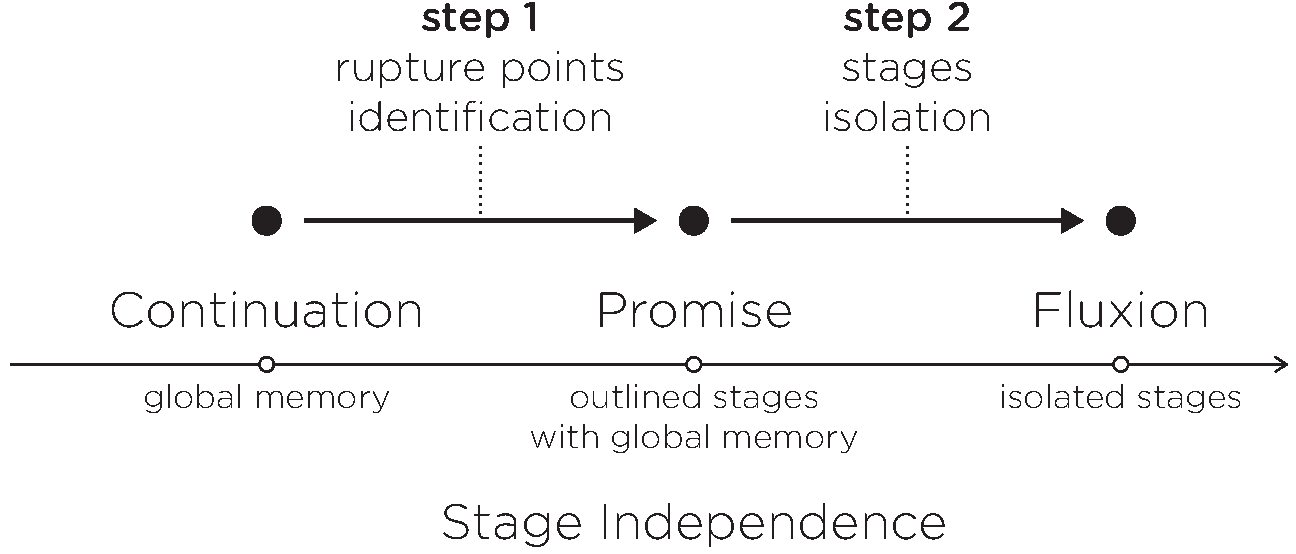
\includegraphics[width=0.7\textwidth]{../resources/roadmap.pdf}%
    \caption{Roadmap}%
    \label{fig:roadmap}%
  }%
\end{figure}

The first compiler focuses on the identification of simple chains of causality between continuations to transform these chains into Promises.
% the transformation from continuations to Promises.
% It focuses on the identification of the chains of causality in continuations.
However, promises are more expressive than the simple chaining of causal sequentiality.
% They force another control over the execution flow.
% According to the outcome of the operation, they call one function to continue the execution with the result, or another to handle errors.
% This conditional execution is indivisible from the Promise specification.
% Promises impose a convention on how to hand back the outcome of the deferred computation, while classic continuations leave this conditional execution to the developer.
Moreover, they impose a different convention than continuations on how to hand back the outcome and errors of the deferred computation.
This difference brings unnecessary complexity to the identification of chains.
To rule out this difference between continuations and Promises, before introducing the first compiler, section \ref{chapter5:due} introduces a simpler specification to Promise, called Due.

The second compiler detects all the chains of causality between continuations and encapsulate them in fluxions.
It isolates the fluxions when possible to allow the parallelism required for efficiency.
This second compilers is introduced in section \ref{chapter5:flx}.

\renewcommand{\glyph}{\iconfont{\XeTeXglyph287}}
\chapter{Implementations} \label{chapter5}
\minitoc
\eject
The transformation allowed by the equivalence from an event-driven program into a distributed network of fluxions is implemented incrementally into two compilers, as presented in figure \ref{fig:roadmap}.
Each compilers is divided into two steps, the identification of the rupture points separating the stages of the pipeline, and the isolation of these stages.
% This chapter presents the technical implementations of these two steps in the transformation from the event-driven execution model to the pipeline architecture
% , the transformation described in the previous chapter was implemented incrementally in two compilers.

\begin{figure}[h!]%
  \textfig{%
    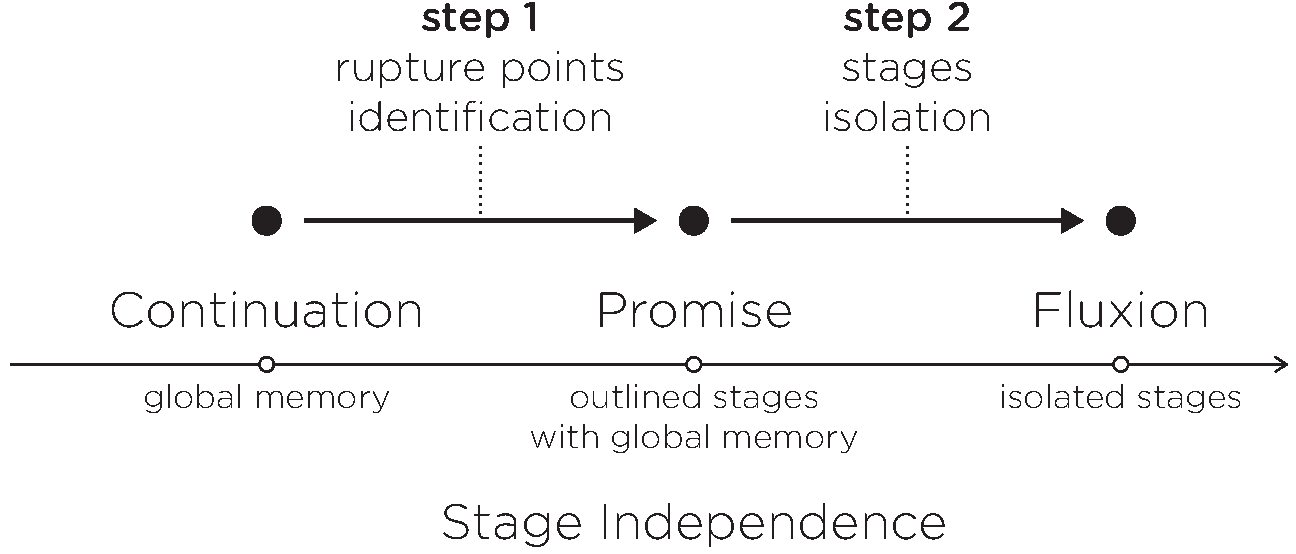
\includegraphics[width=0.7\textwidth]{../resources/roadmap.pdf}%
    \caption{Roadmap}%
    \label{fig:roadmap}%
  }%
\end{figure}

The first compiler focuses on the identification of simple chains of causality between continuations to transform these chains into Promises.
% the transformation from continuations to Promises.
% It focuses on the identification of the chains of causality in continuations.
However, promises are more expressive than the simple chaining of causal sequentiality.
% They force another control over the execution flow.
% According to the outcome of the operation, they call one function to continue the execution with the result, or another to handle errors.
% This conditional execution is indivisible from the Promise specification.
% Promises impose a convention on how to hand back the outcome of the deferred computation, while classic continuations leave this conditional execution to the developer.
Moreover, they impose a different convention than continuations on how to hand back the outcome and errors of the deferred computation.
This difference brings unnecessary complexity to the identification of chains.
To rule out this difference between continuations and Promises, before introducing the first compiler, section \ref{chapter5:due} introduces a simpler specification to Promise, called Due.

The second compiler detects all the chains of causality between continuations and encapsulate them in fluxions.
It isolates the fluxions when possible to allow the parallelism required for efficiency.
This second compilers is introduced in section \ref{chapter5:flx}.

\renewcommand{\glyph}{\iconfont{\XeTeXglyph287}}
\chapter{Implementations} \label{chapter5}
\minitoc
\eject
The transformation allowed by the equivalence from an event-driven program into a distributed network of fluxions is implemented incrementally into two compilers, as presented in figure \ref{fig:roadmap}.
Each compilers is divided into two steps, the identification of the rupture points separating the stages of the pipeline, and the isolation of these stages.
% This chapter presents the technical implementations of these two steps in the transformation from the event-driven execution model to the pipeline architecture
% , the transformation described in the previous chapter was implemented incrementally in two compilers.

\begin{figure}[h!]%
  \textfig{%
    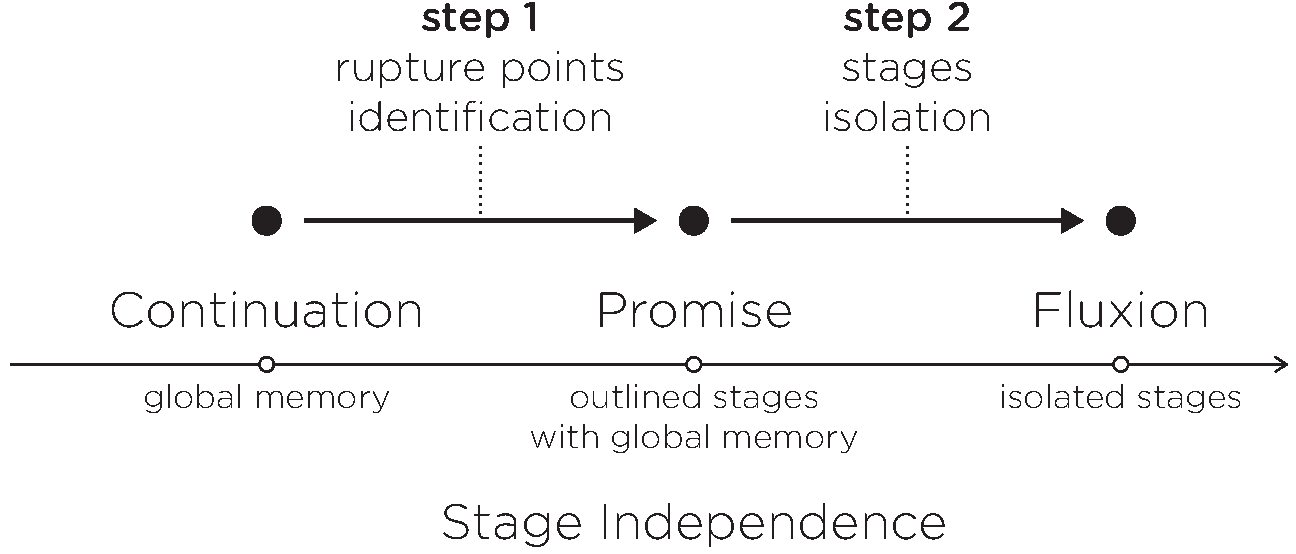
\includegraphics[width=0.7\textwidth]{../resources/roadmap.pdf}%
    \caption{Roadmap}%
    \label{fig:roadmap}%
  }%
\end{figure}

The first compiler focuses on the identification of simple chains of causality between continuations to transform these chains into Promises.
% the transformation from continuations to Promises.
% It focuses on the identification of the chains of causality in continuations.
However, promises are more expressive than the simple chaining of causal sequentiality.
% They force another control over the execution flow.
% According to the outcome of the operation, they call one function to continue the execution with the result, or another to handle errors.
% This conditional execution is indivisible from the Promise specification.
% Promises impose a convention on how to hand back the outcome of the deferred computation, while classic continuations leave this conditional execution to the developer.
Moreover, they impose a different convention than continuations on how to hand back the outcome and errors of the deferred computation.
This difference brings unnecessary complexity to the identification of chains.
To rule out this difference between continuations and Promises, before introducing the first compiler, section \ref{chapter5:due} introduces a simpler specification to Promise, called Due.

The second compiler detects all the chains of causality between continuations and encapsulate them in fluxions.
It isolates the fluxions when possible to allow the parallelism required for efficiency.
This second compilers is introduced in section \ref{chapter5:flx}.

\input{05-implementation/Due/main}
\input{05-implementation/Flx/main}
% \input{05-implementation/Evaluation}

\renewcommand{\glyph}{\iconfont{\XeTeXglyph287}}
\chapter{Implementations} \label{chapter5}
\minitoc
\eject
The transformation allowed by the equivalence from an event-driven program into a distributed network of fluxions is implemented incrementally into two compilers, as presented in figure \ref{fig:roadmap}.
Each compilers is divided into two steps, the identification of the rupture points separating the stages of the pipeline, and the isolation of these stages.
% This chapter presents the technical implementations of these two steps in the transformation from the event-driven execution model to the pipeline architecture
% , the transformation described in the previous chapter was implemented incrementally in two compilers.

\begin{figure}[h!]%
  \textfig{%
    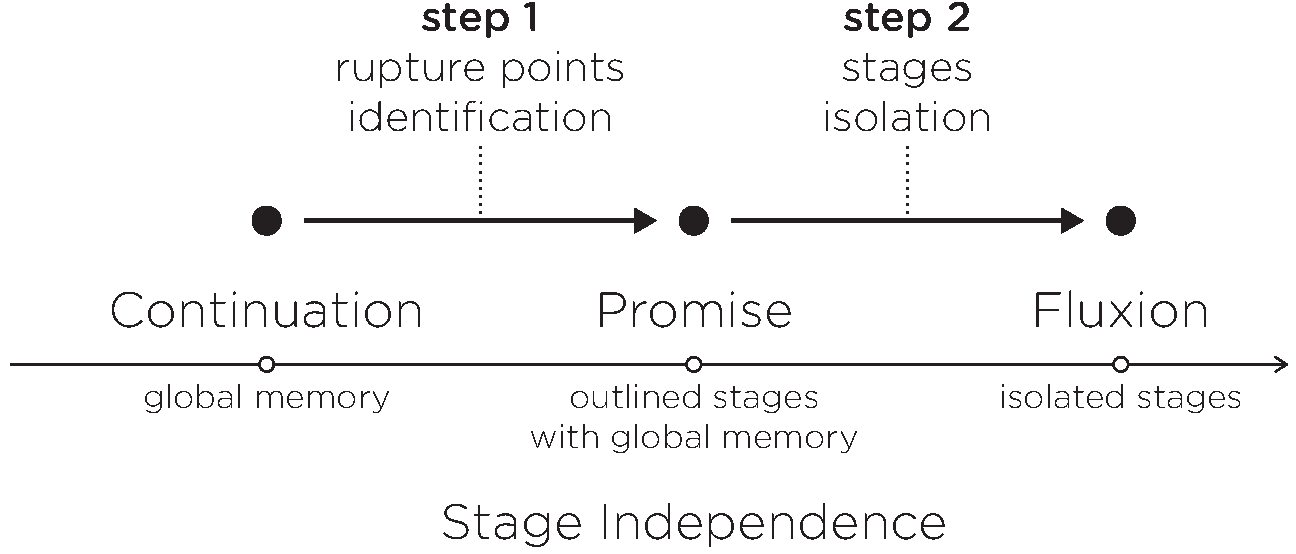
\includegraphics[width=0.7\textwidth]{../resources/roadmap.pdf}%
    \caption{Roadmap}%
    \label{fig:roadmap}%
  }%
\end{figure}

The first compiler focuses on the identification of simple chains of causality between continuations to transform these chains into Promises.
% the transformation from continuations to Promises.
% It focuses on the identification of the chains of causality in continuations.
However, promises are more expressive than the simple chaining of causal sequentiality.
% They force another control over the execution flow.
% According to the outcome of the operation, they call one function to continue the execution with the result, or another to handle errors.
% This conditional execution is indivisible from the Promise specification.
% Promises impose a convention on how to hand back the outcome of the deferred computation, while classic continuations leave this conditional execution to the developer.
Moreover, they impose a different convention than continuations on how to hand back the outcome and errors of the deferred computation.
This difference brings unnecessary complexity to the identification of chains.
To rule out this difference between continuations and Promises, before introducing the first compiler, section \ref{chapter5:due} introduces a simpler specification to Promise, called Due.

The second compiler detects all the chains of causality between continuations and encapsulate them in fluxions.
It isolates the fluxions when possible to allow the parallelism required for efficiency.
This second compilers is introduced in section \ref{chapter5:flx}.

\input{05-implementation/Due/main}
\input{05-implementation/Flx/main}
% \input{05-implementation/Evaluation}

% \subsection{Real test case} \label{chapter5:flx:evaluation}

The compiler is tested on a real application, gifsockets-server\ftnt{https://github.com/twolfson/gifsockets-server}.
This test proves the possibility for an application to be compiled into a network of independent parts.
It shows the current limitations of this isolation and the modifications needed on the application to circumvent them.

\begin{code}[js, caption={Simplified version of gifsockets-server},label={lst:gifsocket}]
var express = require('express'),
    app = express(),
    routes = require('gifsockets-middleware'), //@\label{lst:gifsocket:gif-mw}@
    getRawBody = require('raw-body');

function bodyParser(limit) { //@\label{lst:gifsocket:bodyParser}@
  return function saveBody(req, res, next) { //@\label{lst:gifsocket:saveBody}@
    getRawBody(req, { //@\label{lst:gifsocket:getRawBody}@
      expected: req.headers['content-length'],
      limit: limit
    }, function (err, buffer) { //@\label{lst:gifsocket:callback}@
      req.body = buffer;
      next(); //@\label{lst:gifsocket:next}@
    });
  };
}

app.post('/image/text', bodyParser(1 * 1024 * 1024), routes.writeTextToImages); //@\label{lst:gifsocket:app.post}@
app.listen(8000);
\end{code}

This application, simplified in listing \ref{lst:gifsocket}, is a real-time chat using gif-based communication channels.
It was selected from the evaluation set of the Due compiler because it is simple enough to illustrate this evaluation.
% \cite{Brodu2015}
%  from the \texttt{npm} registry because it depends on \texttt{express}, it is tested, working, and simple enough to illustrate this evaluation.
The server transforms the received text into a gif frame, and pushes it back to a never-ending gif to be displayed on the client.

On line \ref{lst:gifsocket:app.post}, the application registers two functions to process the requests received on the url \texttt{/image/text}.
The closure \texttt{saveBody}, line \ref{lst:gifsocket:saveBody}, returned by \texttt{bodyParser}, line \ref{lst:gifsocket:bodyParser}, and the method \texttt{routes.write\-Text\-To\-Images} from the external module \texttt{gifsockets-\-middleware}, line \ref{lst:gifsocket:gif-mw}.
The closure \texttt{saveBody} calls the asynchronous function \texttt{getRawBody} to get the request body.
Its callback handles the errors, and calls \texttt{next} to continue processing the request with the next function, \texttt{routes.write\-Text\-To\-Images}.

\subsubsection{Compilation} \label{chapter5:flx:evaluation:compilation}

% We compile this application with the compiler
The compilation result is in listing \ref{lst:flx-gifsocket}.
The function call \texttt{app.post}, line \ref{lst:gifsocket:app.post}, is a rupture point.
However, its callbacks, \texttt{bodyParser} and \texttt{routes.write\-Text\-To\-Images} are not declared \textit{in situ}.
They are evaluated as functions only at runtime.
As precised previously, the compiler discards these callbacks to avoid altering the semantic. % by moving or modifying their definition.
% For this reason, the compiler ignores this rupture point, to avoid interfering with the evaluation.

\begin{code}[flx, caption={Compilation result of gifsockets-server},label={lst:flx-gifsocket}]
flx main & express {req}
>> anonymous_1000 [req, next]
  var express = require('express'),
      app = express(),
      routes = require('gifsockets-middleware'), //@\label{lst:flx-gifsocket:gif-mw}@
      getRawBody = require('raw-body');

  function bodyParser(limit) { //@\label{lst:flx-gifsocket:bodyParser}@
    return function saveBody(req, res, next) { //@\label{lst:flx-gifsocket:saveBody}@
      getRawBody(req, { //@\label{lst:flx-gifsocket:getRawBody}@
        expected: req.headers['content-length'], //@\label{lst:flx-gifsocket:req.headers}@
        limit: limit
      }, >> anonymous_1000 [req, next]);
    };
  }

  app.post('/image/text', bodyParser(1 * 1024 * 1024), routes.writeTextToImages); //@\label{lst:flx-gifsocket:app.post}@
  app.listen(8000);

flx anonymous_1000
-> null
  function (err, buffer) { //@\label{lst:flx-gifsocket:callback}@
    req.body = buffer; //@\label{lst:flx-gifsocket:buffer}@
    next(); //@\label{lst:flx-gifsocket:next}@
  }
\end{code}

The compiler detects a rupture point : the function \texttt{get\-Raw\-Body} and its anonymous callback, line \ref{lst:gifsocket:callback}.
It encapsulates this callback in a fluxion named \texttt{anony\-mous\_\-1000}.
The callback is replaced with a stream placeholder to send the message stream to this downstream fluxion.
The variables \texttt{req} and \texttt{next} are appended to this message stream, to propagate their value from the \texttt{main} fluxion to the \texttt{anony\-mous\_\-1000} fluxion.

When \texttt{anony\-mous\_\-1000} is not isolated from the \texttt{main} fluxion, as if they belong to the same group, the compilation result works as expected.
The variables used in the fluxion, \texttt{req} and \texttt{next}, are still shared between the two fluxions.
In this situation fluxions are quite similar to Dues regarding memory shareing.
Our goal is to isolate the two fluxions, to be able to safely parallelize their executions.

\subsubsection{Isolation} \label{chapter5:flx:evaluation:isolation}

In listing \ref{lst:flx-gifsocket}, the fluxion \texttt{anony\-mous\_\-1000} modifies the object \texttt{req}, line \ref{lst:flx-gifsocket:buffer}, to store the text of the received request, and it calls \texttt{next} to continue the execution, line \ref{lst:flx-gifsocket:next}.
\texttt{req} is an alias to a memory location used in multiple palces in code.
Therefore, these operations produce side-effects that should propagate in the whole application, but the isolation prevents this propagation.
Isolating the fluxion \texttt{anony\-mous\_\-1000} produces runtime exceptions.
The next paragraph details how this situation is handled to allow the application to be parallelized.

\paragraph{Variable \texttt{req}}

The variable \texttt{req} is read in fluxion \texttt{main}, lines \ref{lst:flx-gifsocket:getRawBody} and \ref{lst:flx-gifsocket:req.headers}.
Then its property \texttt{body} is associated to \texttt{buffer} in fluxion \texttt{anony\-mous\_\-1000}, line \ref{lst:flx-gifsocket:buffer}.
The compiler is unable to identify the aliases of this variable. % further usages.
However, the side effect resulting from this association impacts a variable in the scope of the next callback, \texttt{routes.write\-Text\-To\-Images}.
In this test case, the application is modified manually to explicitly propagate this side-effect to the next callback through the function \texttt{next}.
The modifications of this function are explained further in the next paragraph.

\paragraph{Closure \texttt{next}}

The function \texttt{next} is a closure provided by the \texttt{express} \texttt{Router} to continue the execution with the next function to handle the client request.
Because it indirectly relies on the variable \texttt{req}, it is impossible to isolate its execution with the \texttt{anony\-mous\_\-1000} fluxion.
Instead, we modify \texttt{express}, so as to be compatible with the fluxional execution model.
We explain the modifications below.

\begin{code}[flx, caption={Simplified modification on the compiled result},label={lst:mflx-gifsocket}]
flx anonymous_1000
-> express_dispatcher
  function (err, buffer) { //@\label{lst:mflx-gifsocket:callback}@
    req.body = buffer; //@\label{lst:mflx-gifsocket:buffer}@
    next_placeholder(req, -> express_dispatcher); //@\label{lst:mflx-gifsocket:next-placeholder}@
  }

flx express_dispatcher & express {req} //@\label{lst:mflx-gifsocket:express-dispatcher}@
-> null
  function (modified_req) {
    merge(req, modified_req);
    next(); //@\label{lst:mflx-gifsocket:next}@
  }
\end{code}

In listing \ref{lst:gifsocket}, the function \texttt{next} is a continuation allowing the anonymous callback, line \ref{lst:gifsocket:callback}, to call the next function to handle the request.
To isolate the anonymous callback into \texttt{anonymous\_\-1000}, \texttt{next} is replaced by a rupture point.
This replacement is illustrated in listing \ref{lst:mflx-gifsocket}.
The \texttt{express} \texttt{Router} registers a fluxion named \texttt{express\_\-dispatcher}, line \ref{lst:mflx-gifsocket:express-dispatcher}, to continue the execution after the fluxion \texttt{anony\-mous\_\-1000}.
This fluxion is in the same group \texttt{express} as the \texttt{main} fluxion, hence it has access to the original variable \texttt{req}, and to the original function \texttt{next}.
The call to the original \texttt{next} function is replaced by a placeholder to push the stream to the fluxion \texttt{express\_\-dispatcher}, line \ref{lst:mflx-gifsocket:next-placeholder}.
The fluxion \texttt{express\_\-dispatcher} receives the stream from the upstream fluxion \texttt{anony\-mous\_\-1000}, merges back the modification in the variable \texttt{req} to propagate the side effects, and finally calls the original function \texttt{next} to continue the execution, line \ref{lst:mflx-gifsocket:next}.

After the modifications detailed above, the server works as expected.
The isolated fluxion correctly receives, and returns its serialized messages.
The client successfully receives a gif frame containing the text.



\subsection{Limitations}

The static analysis used for this compiler presents some limitations.
It is unable to analyze code with dynamic behaviors.
Higher-order programming leads to more productivity partly beacuse it rely on such dynamic behavior to extend expressivity.
Precisely, it allows more levels of indirections.

\subsubsection{Levels of Indirections}

The indirection is an abstraction between the value, and its manipulation.
In listing \ref{lst:indirection}, the variables \texttt{a} and \texttt{b} point both to the same memory object.
The function \texttt{fn} introduces a level of indirection between the real object \texttt{a} and its manipulation handle, \texttt{b};
% Actually, the variable \texttt{a} already introduces a level of indirection between the real object and the handle \texttt{a}.

\begin{code}[js,
  caption={One level of Indirection},
  label={lst:indirection}]
var a = {
      // an object;
    };

fn(b) {
  // modify b;
}

fn(a);
\end{code}

\subsubsection{Uncertainties}

The indirection is trivial to resolve in listing \ref{lst:indirection}.
It only needs to have access to the definition of \texttt{a} and of \texttt{fn}.
%A very simple static analysis could resolve it.
However, in listing \ref{lst:indirections}, the array \texttt{handlers} introduces a new level of indirection.
The static analysis now needs to have access to the definition of \texttt{i} and of the \texttt{handlers}.
If this definition is provided by an external input, it is not available statically, hence, it adds an uncertainty during the analysis. 

\begin{code}[js,
  caption={Two levels of indirection},
  label={lst:indirections}]
var a = {
      // an object;
    },
    handlers = [
      // definition of fn handlers;
    ],
    i = ?;

handlers[i](a);
handlers[i+1](a);
\end{code}

These examples are extremely simplified.
A real application contains enough indirections for the static analysis to be overwhelmed by uncertainties, and to be unable to resolve the variables.
If a variable is left unresolved, it is impossible to assure its scope and its aliases.
Therefore, the compiler is unable to isolate it into a fluxion, or to distribute its modification by messages.

Moreover, it leads the compiler to ignore the rupture points not defined \textit{in situ}, because their modifications could impact the semantic.
The reason for this precaution, is that the compiler is unable to assure where the function is used, and the scope of its variables.
Therefore, it is unable to assure that the modification will conserve the semantic.

\subsubsection{Dynamic Resolution}

In a web application, this variable \texttt{i} might be part of the user request, which is available only at runtime.
It eventually introduces an uncertainty.

This dynamic resolution of variables is precisely what increase expressiveness.
Trying to resolve them statically is equivalent to restrict expressiveness.
No static analysis can overstep these limitations.
Only a dynamic analysis could analysis the resolved indirections during run time to overstep these limitations correctly.




\renewcommand{\glyph}{\iconfont{\XeTeXglyph287}}
\chapter{Implementations} \label{chapter5}
\minitoc
\eject
The transformation allowed by the equivalence from an event-driven program into a distributed network of fluxions is implemented incrementally into two compilers, as presented in figure \ref{fig:roadmap}.
Each compilers is divided into two steps, the identification of the rupture points separating the stages of the pipeline, and the isolation of these stages.
% This chapter presents the technical implementations of these two steps in the transformation from the event-driven execution model to the pipeline architecture
% , the transformation described in the previous chapter was implemented incrementally in two compilers.

\begin{figure}[h!]%
  \textfig{%
    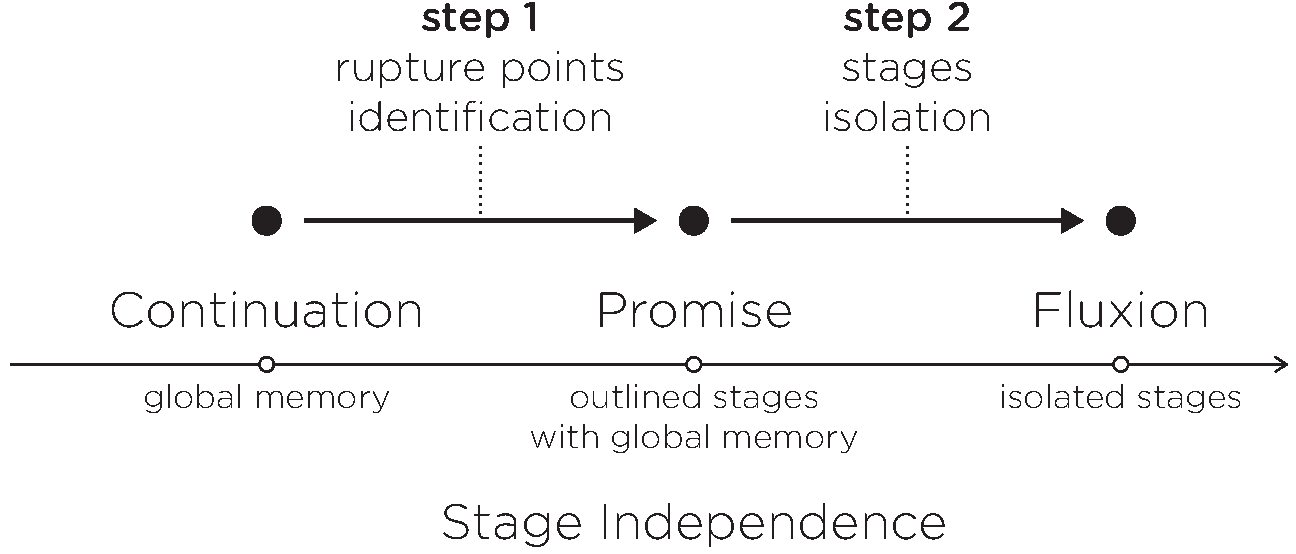
\includegraphics[width=0.7\textwidth]{../resources/roadmap.pdf}%
    \caption{Roadmap}%
    \label{fig:roadmap}%
  }%
\end{figure}

The first compiler focuses on the identification of simple chains of causality between continuations to transform these chains into Promises.
% the transformation from continuations to Promises.
% It focuses on the identification of the chains of causality in continuations.
However, promises are more expressive than the simple chaining of causal sequentiality.
% They force another control over the execution flow.
% According to the outcome of the operation, they call one function to continue the execution with the result, or another to handle errors.
% This conditional execution is indivisible from the Promise specification.
% Promises impose a convention on how to hand back the outcome of the deferred computation, while classic continuations leave this conditional execution to the developer.
Moreover, they impose a different convention than continuations on how to hand back the outcome and errors of the deferred computation.
This difference brings unnecessary complexity to the identification of chains.
To rule out this difference between continuations and Promises, before introducing the first compiler, section \ref{chapter5:due} introduces a simpler specification to Promise, called Due.

The second compiler detects all the chains of causality between continuations and encapsulate them in fluxions.
It isolates the fluxions when possible to allow the parallelism required for efficiency.
This second compilers is introduced in section \ref{chapter5:flx}.

\renewcommand{\glyph}{\iconfont{\XeTeXglyph287}}
\chapter{Implementations} \label{chapter5}
\minitoc
\eject
The transformation allowed by the equivalence from an event-driven program into a distributed network of fluxions is implemented incrementally into two compilers, as presented in figure \ref{fig:roadmap}.
Each compilers is divided into two steps, the identification of the rupture points separating the stages of the pipeline, and the isolation of these stages.
% This chapter presents the technical implementations of these two steps in the transformation from the event-driven execution model to the pipeline architecture
% , the transformation described in the previous chapter was implemented incrementally in two compilers.

\begin{figure}[h!]%
  \textfig{%
    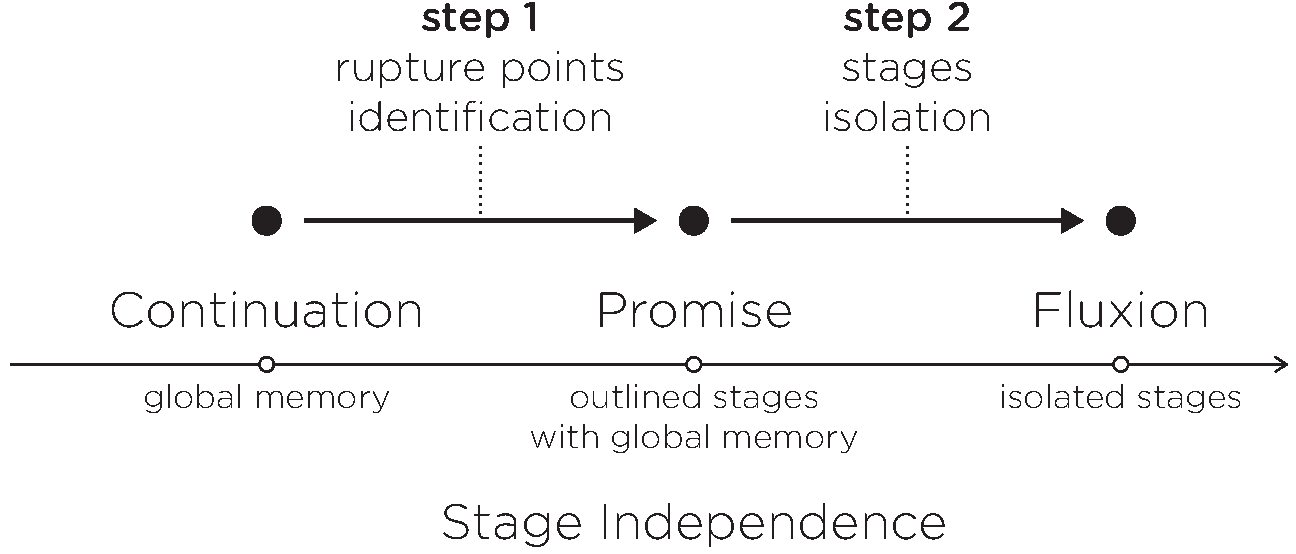
\includegraphics[width=0.7\textwidth]{../resources/roadmap.pdf}%
    \caption{Roadmap}%
    \label{fig:roadmap}%
  }%
\end{figure}

The first compiler focuses on the identification of simple chains of causality between continuations to transform these chains into Promises.
% the transformation from continuations to Promises.
% It focuses on the identification of the chains of causality in continuations.
However, promises are more expressive than the simple chaining of causal sequentiality.
% They force another control over the execution flow.
% According to the outcome of the operation, they call one function to continue the execution with the result, or another to handle errors.
% This conditional execution is indivisible from the Promise specification.
% Promises impose a convention on how to hand back the outcome of the deferred computation, while classic continuations leave this conditional execution to the developer.
Moreover, they impose a different convention than continuations on how to hand back the outcome and errors of the deferred computation.
This difference brings unnecessary complexity to the identification of chains.
To rule out this difference between continuations and Promises, before introducing the first compiler, section \ref{chapter5:due} introduces a simpler specification to Promise, called Due.

The second compiler detects all the chains of causality between continuations and encapsulate them in fluxions.
It isolates the fluxions when possible to allow the parallelism required for efficiency.
This second compilers is introduced in section \ref{chapter5:flx}.

\input{05-implementation/Due/main}
\input{05-implementation/Flx/main}
% \input{05-implementation/Evaluation}

\renewcommand{\glyph}{\iconfont{\XeTeXglyph287}}
\chapter{Implementations} \label{chapter5}
\minitoc
\eject
The transformation allowed by the equivalence from an event-driven program into a distributed network of fluxions is implemented incrementally into two compilers, as presented in figure \ref{fig:roadmap}.
Each compilers is divided into two steps, the identification of the rupture points separating the stages of the pipeline, and the isolation of these stages.
% This chapter presents the technical implementations of these two steps in the transformation from the event-driven execution model to the pipeline architecture
% , the transformation described in the previous chapter was implemented incrementally in two compilers.

\begin{figure}[h!]%
  \textfig{%
    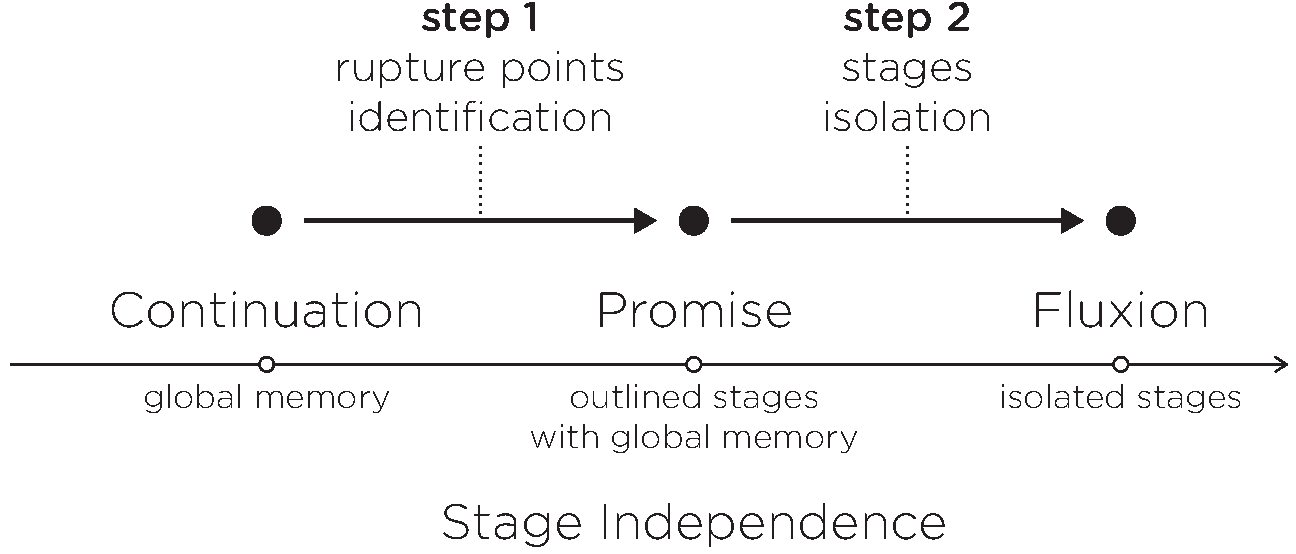
\includegraphics[width=0.7\textwidth]{../resources/roadmap.pdf}%
    \caption{Roadmap}%
    \label{fig:roadmap}%
  }%
\end{figure}

The first compiler focuses on the identification of simple chains of causality between continuations to transform these chains into Promises.
% the transformation from continuations to Promises.
% It focuses on the identification of the chains of causality in continuations.
However, promises are more expressive than the simple chaining of causal sequentiality.
% They force another control over the execution flow.
% According to the outcome of the operation, they call one function to continue the execution with the result, or another to handle errors.
% This conditional execution is indivisible from the Promise specification.
% Promises impose a convention on how to hand back the outcome of the deferred computation, while classic continuations leave this conditional execution to the developer.
Moreover, they impose a different convention than continuations on how to hand back the outcome and errors of the deferred computation.
This difference brings unnecessary complexity to the identification of chains.
To rule out this difference between continuations and Promises, before introducing the first compiler, section \ref{chapter5:due} introduces a simpler specification to Promise, called Due.

The second compiler detects all the chains of causality between continuations and encapsulate them in fluxions.
It isolates the fluxions when possible to allow the parallelism required for efficiency.
This second compilers is introduced in section \ref{chapter5:flx}.

\input{05-implementation/Due/main}
\input{05-implementation/Flx/main}
% \input{05-implementation/Evaluation}

% \subsection{Real test case} \label{chapter5:flx:evaluation}

The compiler is tested on a real application, gifsockets-server\ftnt{https://github.com/twolfson/gifsockets-server}.
This test proves the possibility for an application to be compiled into a network of independent parts.
It shows the current limitations of this isolation and the modifications needed on the application to circumvent them.

\begin{code}[js, caption={Simplified version of gifsockets-server},label={lst:gifsocket}]
var express = require('express'),
    app = express(),
    routes = require('gifsockets-middleware'), //@\label{lst:gifsocket:gif-mw}@
    getRawBody = require('raw-body');

function bodyParser(limit) { //@\label{lst:gifsocket:bodyParser}@
  return function saveBody(req, res, next) { //@\label{lst:gifsocket:saveBody}@
    getRawBody(req, { //@\label{lst:gifsocket:getRawBody}@
      expected: req.headers['content-length'],
      limit: limit
    }, function (err, buffer) { //@\label{lst:gifsocket:callback}@
      req.body = buffer;
      next(); //@\label{lst:gifsocket:next}@
    });
  };
}

app.post('/image/text', bodyParser(1 * 1024 * 1024), routes.writeTextToImages); //@\label{lst:gifsocket:app.post}@
app.listen(8000);
\end{code}

This application, simplified in listing \ref{lst:gifsocket}, is a real-time chat using gif-based communication channels.
It was selected from the evaluation set of the Due compiler because it is simple enough to illustrate this evaluation.
% \cite{Brodu2015}
%  from the \texttt{npm} registry because it depends on \texttt{express}, it is tested, working, and simple enough to illustrate this evaluation.
The server transforms the received text into a gif frame, and pushes it back to a never-ending gif to be displayed on the client.

On line \ref{lst:gifsocket:app.post}, the application registers two functions to process the requests received on the url \texttt{/image/text}.
The closure \texttt{saveBody}, line \ref{lst:gifsocket:saveBody}, returned by \texttt{bodyParser}, line \ref{lst:gifsocket:bodyParser}, and the method \texttt{routes.write\-Text\-To\-Images} from the external module \texttt{gifsockets-\-middleware}, line \ref{lst:gifsocket:gif-mw}.
The closure \texttt{saveBody} calls the asynchronous function \texttt{getRawBody} to get the request body.
Its callback handles the errors, and calls \texttt{next} to continue processing the request with the next function, \texttt{routes.write\-Text\-To\-Images}.

\subsubsection{Compilation} \label{chapter5:flx:evaluation:compilation}

% We compile this application with the compiler
The compilation result is in listing \ref{lst:flx-gifsocket}.
The function call \texttt{app.post}, line \ref{lst:gifsocket:app.post}, is a rupture point.
However, its callbacks, \texttt{bodyParser} and \texttt{routes.write\-Text\-To\-Images} are not declared \textit{in situ}.
They are evaluated as functions only at runtime.
As precised previously, the compiler discards these callbacks to avoid altering the semantic. % by moving or modifying their definition.
% For this reason, the compiler ignores this rupture point, to avoid interfering with the evaluation.

\begin{code}[flx, caption={Compilation result of gifsockets-server},label={lst:flx-gifsocket}]
flx main & express {req}
>> anonymous_1000 [req, next]
  var express = require('express'),
      app = express(),
      routes = require('gifsockets-middleware'), //@\label{lst:flx-gifsocket:gif-mw}@
      getRawBody = require('raw-body');

  function bodyParser(limit) { //@\label{lst:flx-gifsocket:bodyParser}@
    return function saveBody(req, res, next) { //@\label{lst:flx-gifsocket:saveBody}@
      getRawBody(req, { //@\label{lst:flx-gifsocket:getRawBody}@
        expected: req.headers['content-length'], //@\label{lst:flx-gifsocket:req.headers}@
        limit: limit
      }, >> anonymous_1000 [req, next]);
    };
  }

  app.post('/image/text', bodyParser(1 * 1024 * 1024), routes.writeTextToImages); //@\label{lst:flx-gifsocket:app.post}@
  app.listen(8000);

flx anonymous_1000
-> null
  function (err, buffer) { //@\label{lst:flx-gifsocket:callback}@
    req.body = buffer; //@\label{lst:flx-gifsocket:buffer}@
    next(); //@\label{lst:flx-gifsocket:next}@
  }
\end{code}

The compiler detects a rupture point : the function \texttt{get\-Raw\-Body} and its anonymous callback, line \ref{lst:gifsocket:callback}.
It encapsulates this callback in a fluxion named \texttt{anony\-mous\_\-1000}.
The callback is replaced with a stream placeholder to send the message stream to this downstream fluxion.
The variables \texttt{req} and \texttt{next} are appended to this message stream, to propagate their value from the \texttt{main} fluxion to the \texttt{anony\-mous\_\-1000} fluxion.

When \texttt{anony\-mous\_\-1000} is not isolated from the \texttt{main} fluxion, as if they belong to the same group, the compilation result works as expected.
The variables used in the fluxion, \texttt{req} and \texttt{next}, are still shared between the two fluxions.
In this situation fluxions are quite similar to Dues regarding memory shareing.
Our goal is to isolate the two fluxions, to be able to safely parallelize their executions.

\subsubsection{Isolation} \label{chapter5:flx:evaluation:isolation}

In listing \ref{lst:flx-gifsocket}, the fluxion \texttt{anony\-mous\_\-1000} modifies the object \texttt{req}, line \ref{lst:flx-gifsocket:buffer}, to store the text of the received request, and it calls \texttt{next} to continue the execution, line \ref{lst:flx-gifsocket:next}.
\texttt{req} is an alias to a memory location used in multiple palces in code.
Therefore, these operations produce side-effects that should propagate in the whole application, but the isolation prevents this propagation.
Isolating the fluxion \texttt{anony\-mous\_\-1000} produces runtime exceptions.
The next paragraph details how this situation is handled to allow the application to be parallelized.

\paragraph{Variable \texttt{req}}

The variable \texttt{req} is read in fluxion \texttt{main}, lines \ref{lst:flx-gifsocket:getRawBody} and \ref{lst:flx-gifsocket:req.headers}.
Then its property \texttt{body} is associated to \texttt{buffer} in fluxion \texttt{anony\-mous\_\-1000}, line \ref{lst:flx-gifsocket:buffer}.
The compiler is unable to identify the aliases of this variable. % further usages.
However, the side effect resulting from this association impacts a variable in the scope of the next callback, \texttt{routes.write\-Text\-To\-Images}.
In this test case, the application is modified manually to explicitly propagate this side-effect to the next callback through the function \texttt{next}.
The modifications of this function are explained further in the next paragraph.

\paragraph{Closure \texttt{next}}

The function \texttt{next} is a closure provided by the \texttt{express} \texttt{Router} to continue the execution with the next function to handle the client request.
Because it indirectly relies on the variable \texttt{req}, it is impossible to isolate its execution with the \texttt{anony\-mous\_\-1000} fluxion.
Instead, we modify \texttt{express}, so as to be compatible with the fluxional execution model.
We explain the modifications below.

\begin{code}[flx, caption={Simplified modification on the compiled result},label={lst:mflx-gifsocket}]
flx anonymous_1000
-> express_dispatcher
  function (err, buffer) { //@\label{lst:mflx-gifsocket:callback}@
    req.body = buffer; //@\label{lst:mflx-gifsocket:buffer}@
    next_placeholder(req, -> express_dispatcher); //@\label{lst:mflx-gifsocket:next-placeholder}@
  }

flx express_dispatcher & express {req} //@\label{lst:mflx-gifsocket:express-dispatcher}@
-> null
  function (modified_req) {
    merge(req, modified_req);
    next(); //@\label{lst:mflx-gifsocket:next}@
  }
\end{code}

In listing \ref{lst:gifsocket}, the function \texttt{next} is a continuation allowing the anonymous callback, line \ref{lst:gifsocket:callback}, to call the next function to handle the request.
To isolate the anonymous callback into \texttt{anonymous\_\-1000}, \texttt{next} is replaced by a rupture point.
This replacement is illustrated in listing \ref{lst:mflx-gifsocket}.
The \texttt{express} \texttt{Router} registers a fluxion named \texttt{express\_\-dispatcher}, line \ref{lst:mflx-gifsocket:express-dispatcher}, to continue the execution after the fluxion \texttt{anony\-mous\_\-1000}.
This fluxion is in the same group \texttt{express} as the \texttt{main} fluxion, hence it has access to the original variable \texttt{req}, and to the original function \texttt{next}.
The call to the original \texttt{next} function is replaced by a placeholder to push the stream to the fluxion \texttt{express\_\-dispatcher}, line \ref{lst:mflx-gifsocket:next-placeholder}.
The fluxion \texttt{express\_\-dispatcher} receives the stream from the upstream fluxion \texttt{anony\-mous\_\-1000}, merges back the modification in the variable \texttt{req} to propagate the side effects, and finally calls the original function \texttt{next} to continue the execution, line \ref{lst:mflx-gifsocket:next}.

After the modifications detailed above, the server works as expected.
The isolated fluxion correctly receives, and returns its serialized messages.
The client successfully receives a gif frame containing the text.



\subsection{Limitations}

The static analysis used for this compiler presents some limitations.
It is unable to analyze code with dynamic behaviors.
Higher-order programming leads to more productivity partly beacuse it rely on such dynamic behavior to extend expressivity.
Precisely, it allows more levels of indirections.

\subsubsection{Levels of Indirections}

The indirection is an abstraction between the value, and its manipulation.
In listing \ref{lst:indirection}, the variables \texttt{a} and \texttt{b} point both to the same memory object.
The function \texttt{fn} introduces a level of indirection between the real object \texttt{a} and its manipulation handle, \texttt{b};
% Actually, the variable \texttt{a} already introduces a level of indirection between the real object and the handle \texttt{a}.

\begin{code}[js,
  caption={One level of Indirection},
  label={lst:indirection}]
var a = {
      // an object;
    };

fn(b) {
  // modify b;
}

fn(a);
\end{code}

\subsubsection{Uncertainties}

The indirection is trivial to resolve in listing \ref{lst:indirection}.
It only needs to have access to the definition of \texttt{a} and of \texttt{fn}.
%A very simple static analysis could resolve it.
However, in listing \ref{lst:indirections}, the array \texttt{handlers} introduces a new level of indirection.
The static analysis now needs to have access to the definition of \texttt{i} and of the \texttt{handlers}.
If this definition is provided by an external input, it is not available statically, hence, it adds an uncertainty during the analysis. 

\begin{code}[js,
  caption={Two levels of indirection},
  label={lst:indirections}]
var a = {
      // an object;
    },
    handlers = [
      // definition of fn handlers;
    ],
    i = ?;

handlers[i](a);
handlers[i+1](a);
\end{code}

These examples are extremely simplified.
A real application contains enough indirections for the static analysis to be overwhelmed by uncertainties, and to be unable to resolve the variables.
If a variable is left unresolved, it is impossible to assure its scope and its aliases.
Therefore, the compiler is unable to isolate it into a fluxion, or to distribute its modification by messages.

Moreover, it leads the compiler to ignore the rupture points not defined \textit{in situ}, because their modifications could impact the semantic.
The reason for this precaution, is that the compiler is unable to assure where the function is used, and the scope of its variables.
Therefore, it is unable to assure that the modification will conserve the semantic.

\subsubsection{Dynamic Resolution}

In a web application, this variable \texttt{i} might be part of the user request, which is available only at runtime.
It eventually introduces an uncertainty.

This dynamic resolution of variables is precisely what increase expressiveness.
Trying to resolve them statically is equivalent to restrict expressiveness.
No static analysis can overstep these limitations.
Only a dynamic analysis could analysis the resolved indirections during run time to overstep these limitations correctly.




% \subsection{Real test case} \label{chapter5:flx:evaluation}

The compiler is tested on a real application, gifsockets-server\ftnt{https://github.com/twolfson/gifsockets-server}.
This test proves the possibility for an application to be compiled into a network of independent parts.
It shows the current limitations of this isolation and the modifications needed on the application to circumvent them.

\begin{code}[js, caption={Simplified version of gifsockets-server},label={lst:gifsocket}]
var express = require('express'),
    app = express(),
    routes = require('gifsockets-middleware'), //@\label{lst:gifsocket:gif-mw}@
    getRawBody = require('raw-body');

function bodyParser(limit) { //@\label{lst:gifsocket:bodyParser}@
  return function saveBody(req, res, next) { //@\label{lst:gifsocket:saveBody}@
    getRawBody(req, { //@\label{lst:gifsocket:getRawBody}@
      expected: req.headers['content-length'],
      limit: limit
    }, function (err, buffer) { //@\label{lst:gifsocket:callback}@
      req.body = buffer;
      next(); //@\label{lst:gifsocket:next}@
    });
  };
}

app.post('/image/text', bodyParser(1 * 1024 * 1024), routes.writeTextToImages); //@\label{lst:gifsocket:app.post}@
app.listen(8000);
\end{code}

This application, simplified in listing \ref{lst:gifsocket}, is a real-time chat using gif-based communication channels.
It was selected from the evaluation set of the Due compiler because it is simple enough to illustrate this evaluation.
% \cite{Brodu2015}
%  from the \texttt{npm} registry because it depends on \texttt{express}, it is tested, working, and simple enough to illustrate this evaluation.
The server transforms the received text into a gif frame, and pushes it back to a never-ending gif to be displayed on the client.

On line \ref{lst:gifsocket:app.post}, the application registers two functions to process the requests received on the url \texttt{/image/text}.
The closure \texttt{saveBody}, line \ref{lst:gifsocket:saveBody}, returned by \texttt{bodyParser}, line \ref{lst:gifsocket:bodyParser}, and the method \texttt{routes.write\-Text\-To\-Images} from the external module \texttt{gifsockets-\-middleware}, line \ref{lst:gifsocket:gif-mw}.
The closure \texttt{saveBody} calls the asynchronous function \texttt{getRawBody} to get the request body.
Its callback handles the errors, and calls \texttt{next} to continue processing the request with the next function, \texttt{routes.write\-Text\-To\-Images}.

\subsubsection{Compilation} \label{chapter5:flx:evaluation:compilation}

% We compile this application with the compiler
The compilation result is in listing \ref{lst:flx-gifsocket}.
The function call \texttt{app.post}, line \ref{lst:gifsocket:app.post}, is a rupture point.
However, its callbacks, \texttt{bodyParser} and \texttt{routes.write\-Text\-To\-Images} are not declared \textit{in situ}.
They are evaluated as functions only at runtime.
As precised previously, the compiler discards these callbacks to avoid altering the semantic. % by moving or modifying their definition.
% For this reason, the compiler ignores this rupture point, to avoid interfering with the evaluation.

\begin{code}[flx, caption={Compilation result of gifsockets-server},label={lst:flx-gifsocket}]
flx main & express {req}
>> anonymous_1000 [req, next]
  var express = require('express'),
      app = express(),
      routes = require('gifsockets-middleware'), //@\label{lst:flx-gifsocket:gif-mw}@
      getRawBody = require('raw-body');

  function bodyParser(limit) { //@\label{lst:flx-gifsocket:bodyParser}@
    return function saveBody(req, res, next) { //@\label{lst:flx-gifsocket:saveBody}@
      getRawBody(req, { //@\label{lst:flx-gifsocket:getRawBody}@
        expected: req.headers['content-length'], //@\label{lst:flx-gifsocket:req.headers}@
        limit: limit
      }, >> anonymous_1000 [req, next]);
    };
  }

  app.post('/image/text', bodyParser(1 * 1024 * 1024), routes.writeTextToImages); //@\label{lst:flx-gifsocket:app.post}@
  app.listen(8000);

flx anonymous_1000
-> null
  function (err, buffer) { //@\label{lst:flx-gifsocket:callback}@
    req.body = buffer; //@\label{lst:flx-gifsocket:buffer}@
    next(); //@\label{lst:flx-gifsocket:next}@
  }
\end{code}

The compiler detects a rupture point : the function \texttt{get\-Raw\-Body} and its anonymous callback, line \ref{lst:gifsocket:callback}.
It encapsulates this callback in a fluxion named \texttt{anony\-mous\_\-1000}.
The callback is replaced with a stream placeholder to send the message stream to this downstream fluxion.
The variables \texttt{req} and \texttt{next} are appended to this message stream, to propagate their value from the \texttt{main} fluxion to the \texttt{anony\-mous\_\-1000} fluxion.

When \texttt{anony\-mous\_\-1000} is not isolated from the \texttt{main} fluxion, as if they belong to the same group, the compilation result works as expected.
The variables used in the fluxion, \texttt{req} and \texttt{next}, are still shared between the two fluxions.
In this situation fluxions are quite similar to Dues regarding memory shareing.
Our goal is to isolate the two fluxions, to be able to safely parallelize their executions.

\subsubsection{Isolation} \label{chapter5:flx:evaluation:isolation}

In listing \ref{lst:flx-gifsocket}, the fluxion \texttt{anony\-mous\_\-1000} modifies the object \texttt{req}, line \ref{lst:flx-gifsocket:buffer}, to store the text of the received request, and it calls \texttt{next} to continue the execution, line \ref{lst:flx-gifsocket:next}.
\texttt{req} is an alias to a memory location used in multiple palces in code.
Therefore, these operations produce side-effects that should propagate in the whole application, but the isolation prevents this propagation.
Isolating the fluxion \texttt{anony\-mous\_\-1000} produces runtime exceptions.
The next paragraph details how this situation is handled to allow the application to be parallelized.

\paragraph{Variable \texttt{req}}

The variable \texttt{req} is read in fluxion \texttt{main}, lines \ref{lst:flx-gifsocket:getRawBody} and \ref{lst:flx-gifsocket:req.headers}.
Then its property \texttt{body} is associated to \texttt{buffer} in fluxion \texttt{anony\-mous\_\-1000}, line \ref{lst:flx-gifsocket:buffer}.
The compiler is unable to identify the aliases of this variable. % further usages.
However, the side effect resulting from this association impacts a variable in the scope of the next callback, \texttt{routes.write\-Text\-To\-Images}.
In this test case, the application is modified manually to explicitly propagate this side-effect to the next callback through the function \texttt{next}.
The modifications of this function are explained further in the next paragraph.

\paragraph{Closure \texttt{next}}

The function \texttt{next} is a closure provided by the \texttt{express} \texttt{Router} to continue the execution with the next function to handle the client request.
Because it indirectly relies on the variable \texttt{req}, it is impossible to isolate its execution with the \texttt{anony\-mous\_\-1000} fluxion.
Instead, we modify \texttt{express}, so as to be compatible with the fluxional execution model.
We explain the modifications below.

\begin{code}[flx, caption={Simplified modification on the compiled result},label={lst:mflx-gifsocket}]
flx anonymous_1000
-> express_dispatcher
  function (err, buffer) { //@\label{lst:mflx-gifsocket:callback}@
    req.body = buffer; //@\label{lst:mflx-gifsocket:buffer}@
    next_placeholder(req, -> express_dispatcher); //@\label{lst:mflx-gifsocket:next-placeholder}@
  }

flx express_dispatcher & express {req} //@\label{lst:mflx-gifsocket:express-dispatcher}@
-> null
  function (modified_req) {
    merge(req, modified_req);
    next(); //@\label{lst:mflx-gifsocket:next}@
  }
\end{code}

In listing \ref{lst:gifsocket}, the function \texttt{next} is a continuation allowing the anonymous callback, line \ref{lst:gifsocket:callback}, to call the next function to handle the request.
To isolate the anonymous callback into \texttt{anonymous\_\-1000}, \texttt{next} is replaced by a rupture point.
This replacement is illustrated in listing \ref{lst:mflx-gifsocket}.
The \texttt{express} \texttt{Router} registers a fluxion named \texttt{express\_\-dispatcher}, line \ref{lst:mflx-gifsocket:express-dispatcher}, to continue the execution after the fluxion \texttt{anony\-mous\_\-1000}.
This fluxion is in the same group \texttt{express} as the \texttt{main} fluxion, hence it has access to the original variable \texttt{req}, and to the original function \texttt{next}.
The call to the original \texttt{next} function is replaced by a placeholder to push the stream to the fluxion \texttt{express\_\-dispatcher}, line \ref{lst:mflx-gifsocket:next-placeholder}.
The fluxion \texttt{express\_\-dispatcher} receives the stream from the upstream fluxion \texttt{anony\-mous\_\-1000}, merges back the modification in the variable \texttt{req} to propagate the side effects, and finally calls the original function \texttt{next} to continue the execution, line \ref{lst:mflx-gifsocket:next}.

After the modifications detailed above, the server works as expected.
The isolated fluxion correctly receives, and returns its serialized messages.
The client successfully receives a gif frame containing the text.



\subsection{Limitations}

The static analysis used for this compiler presents some limitations.
It is unable to analyze code with dynamic behaviors.
Higher-order programming leads to more productivity partly beacuse it rely on such dynamic behavior to extend expressivity.
Precisely, it allows more levels of indirections.

\subsubsection{Levels of Indirections}

The indirection is an abstraction between the value, and its manipulation.
In listing \ref{lst:indirection}, the variables \texttt{a} and \texttt{b} point both to the same memory object.
The function \texttt{fn} introduces a level of indirection between the real object \texttt{a} and its manipulation handle, \texttt{b};
% Actually, the variable \texttt{a} already introduces a level of indirection between the real object and the handle \texttt{a}.

\begin{code}[js,
  caption={One level of Indirection},
  label={lst:indirection}]
var a = {
      // an object;
    };

fn(b) {
  // modify b;
}

fn(a);
\end{code}

\subsubsection{Uncertainties}

The indirection is trivial to resolve in listing \ref{lst:indirection}.
It only needs to have access to the definition of \texttt{a} and of \texttt{fn}.
%A very simple static analysis could resolve it.
However, in listing \ref{lst:indirections}, the array \texttt{handlers} introduces a new level of indirection.
The static analysis now needs to have access to the definition of \texttt{i} and of the \texttt{handlers}.
If this definition is provided by an external input, it is not available statically, hence, it adds an uncertainty during the analysis. 

\begin{code}[js,
  caption={Two levels of indirection},
  label={lst:indirections}]
var a = {
      // an object;
    },
    handlers = [
      // definition of fn handlers;
    ],
    i = ?;

handlers[i](a);
handlers[i+1](a);
\end{code}

These examples are extremely simplified.
A real application contains enough indirections for the static analysis to be overwhelmed by uncertainties, and to be unable to resolve the variables.
If a variable is left unresolved, it is impossible to assure its scope and its aliases.
Therefore, the compiler is unable to isolate it into a fluxion, or to distribute its modification by messages.

Moreover, it leads the compiler to ignore the rupture points not defined \textit{in situ}, because their modifications could impact the semantic.
The reason for this precaution, is that the compiler is unable to assure where the function is used, and the scope of its variables.
Therefore, it is unable to assure that the modification will conserve the semantic.

\subsubsection{Dynamic Resolution}

In a web application, this variable \texttt{i} might be part of the user request, which is available only at runtime.
It eventually introduces an uncertainty.

This dynamic resolution of variables is precisely what increase expressiveness.
Trying to resolve them statically is equivalent to restrict expressiveness.
No static analysis can overstep these limitations.
Only a dynamic analysis could analysis the resolved indirections during run time to overstep these limitations correctly.





\chapter{State of the Art}
  \section{Flow-programming}
    \subsection{Functional reactive programming}
    \subsection{Flow-Based programming}
  \section{Event-based distributed middlewares}
    \subsection{Micro-batch processing}
    \subsection{Stream Processing}
    \subsection{\comment{TODO} Other ?}
  \section{Parallelizing compilers}
    \subsection{\comment{TODO}}


% \renewcommand{\glyph}{\iconfont{\XeTeXglyph287}}
\chapter{Implementations} \label{chapter5}
\minitoc
\eject
The transformation allowed by the equivalence from an event-driven program into a distributed network of fluxions is implemented incrementally into two compilers, as presented in figure \ref{fig:roadmap}.
Each compilers is divided into two steps, the identification of the rupture points separating the stages of the pipeline, and the isolation of these stages.
% This chapter presents the technical implementations of these two steps in the transformation from the event-driven execution model to the pipeline architecture
% , the transformation described in the previous chapter was implemented incrementally in two compilers.

\begin{figure}[h!]%
  \textfig{%
    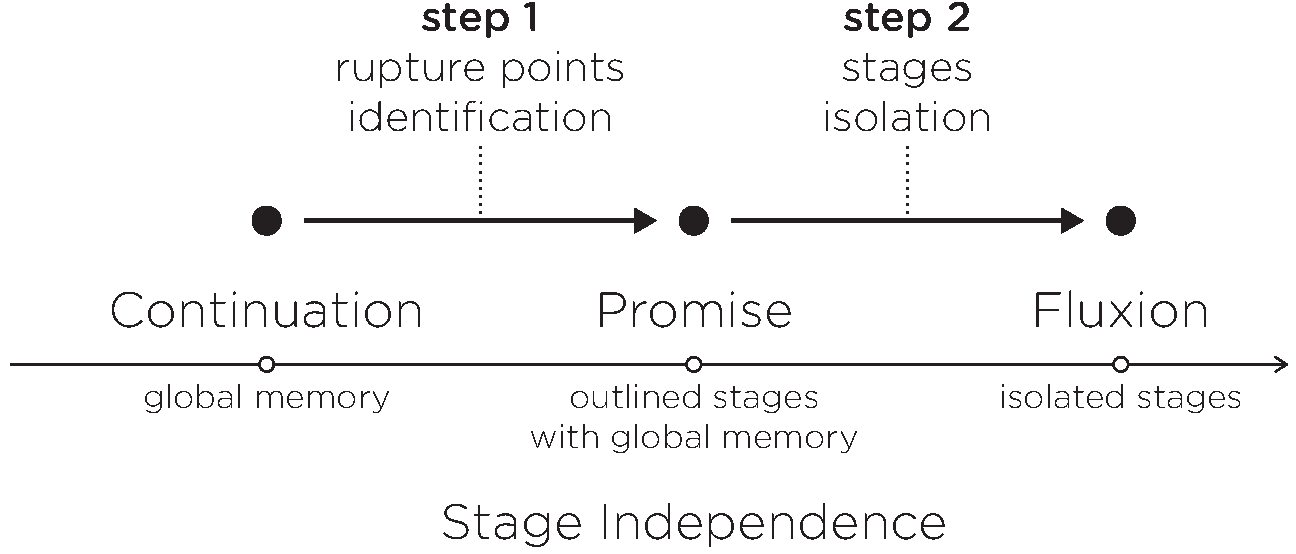
\includegraphics[width=0.7\textwidth]{../resources/roadmap.pdf}%
    \caption{Roadmap}%
    \label{fig:roadmap}%
  }%
\end{figure}

The first compiler focuses on the identification of simple chains of causality between continuations to transform these chains into Promises.
% the transformation from continuations to Promises.
% It focuses on the identification of the chains of causality in continuations.
However, promises are more expressive than the simple chaining of causal sequentiality.
% They force another control over the execution flow.
% According to the outcome of the operation, they call one function to continue the execution with the result, or another to handle errors.
% This conditional execution is indivisible from the Promise specification.
% Promises impose a convention on how to hand back the outcome of the deferred computation, while classic continuations leave this conditional execution to the developer.
Moreover, they impose a different convention than continuations on how to hand back the outcome and errors of the deferred computation.
This difference brings unnecessary complexity to the identification of chains.
To rule out this difference between continuations and Promises, before introducing the first compiler, section \ref{chapter5:due} introduces a simpler specification to Promise, called Due.

The second compiler detects all the chains of causality between continuations and encapsulate them in fluxions.
It isolates the fluxions when possible to allow the parallelism required for efficiency.
This second compilers is introduced in section \ref{chapter5:flx}.

\renewcommand{\glyph}{\iconfont{\XeTeXglyph287}}
\chapter{Implementations} \label{chapter5}
\minitoc
\eject
The transformation allowed by the equivalence from an event-driven program into a distributed network of fluxions is implemented incrementally into two compilers, as presented in figure \ref{fig:roadmap}.
Each compilers is divided into two steps, the identification of the rupture points separating the stages of the pipeline, and the isolation of these stages.
% This chapter presents the technical implementations of these two steps in the transformation from the event-driven execution model to the pipeline architecture
% , the transformation described in the previous chapter was implemented incrementally in two compilers.

\begin{figure}[h!]%
  \textfig{%
    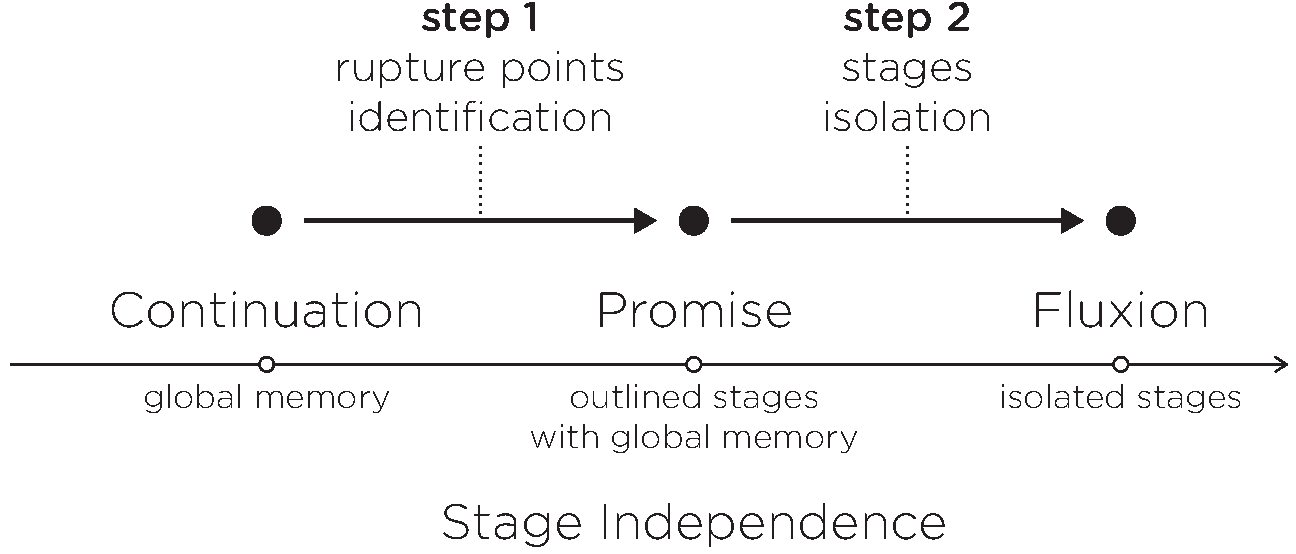
\includegraphics[width=0.7\textwidth]{../resources/roadmap.pdf}%
    \caption{Roadmap}%
    \label{fig:roadmap}%
  }%
\end{figure}

The first compiler focuses on the identification of simple chains of causality between continuations to transform these chains into Promises.
% the transformation from continuations to Promises.
% It focuses on the identification of the chains of causality in continuations.
However, promises are more expressive than the simple chaining of causal sequentiality.
% They force another control over the execution flow.
% According to the outcome of the operation, they call one function to continue the execution with the result, or another to handle errors.
% This conditional execution is indivisible from the Promise specification.
% Promises impose a convention on how to hand back the outcome of the deferred computation, while classic continuations leave this conditional execution to the developer.
Moreover, they impose a different convention than continuations on how to hand back the outcome and errors of the deferred computation.
This difference brings unnecessary complexity to the identification of chains.
To rule out this difference between continuations and Promises, before introducing the first compiler, section \ref{chapter5:due} introduces a simpler specification to Promise, called Due.

The second compiler detects all the chains of causality between continuations and encapsulate them in fluxions.
It isolates the fluxions when possible to allow the parallelism required for efficiency.
This second compilers is introduced in section \ref{chapter5:flx}.

\renewcommand{\glyph}{\iconfont{\XeTeXglyph287}}
\chapter{Implementations} \label{chapter5}
\minitoc
\eject
The transformation allowed by the equivalence from an event-driven program into a distributed network of fluxions is implemented incrementally into two compilers, as presented in figure \ref{fig:roadmap}.
Each compilers is divided into two steps, the identification of the rupture points separating the stages of the pipeline, and the isolation of these stages.
% This chapter presents the technical implementations of these two steps in the transformation from the event-driven execution model to the pipeline architecture
% , the transformation described in the previous chapter was implemented incrementally in two compilers.

\begin{figure}[h!]%
  \textfig{%
    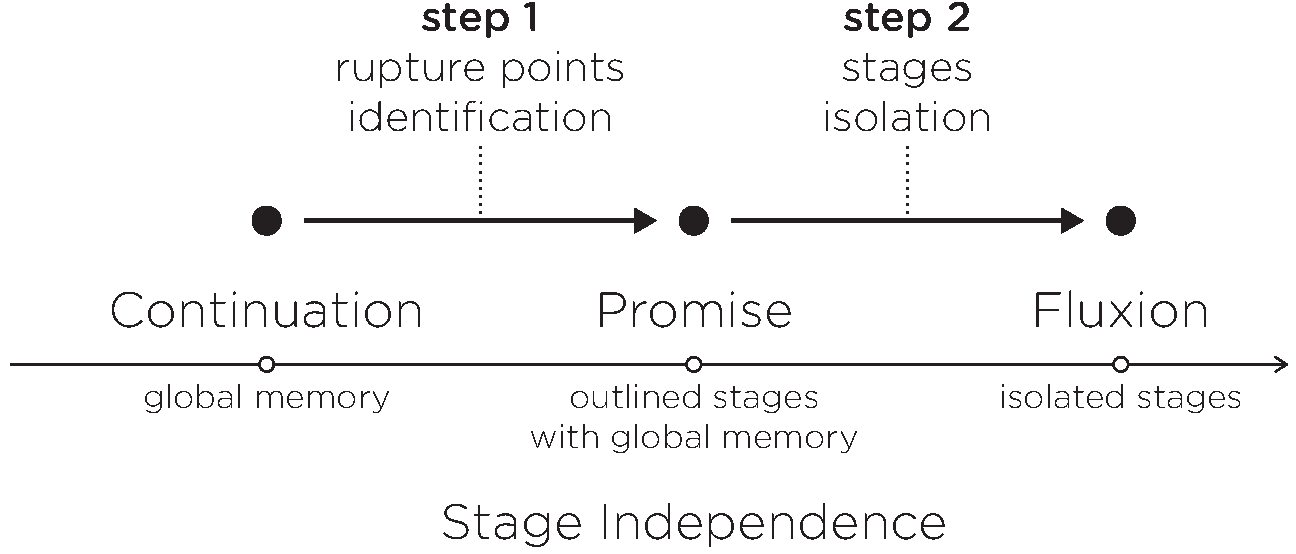
\includegraphics[width=0.7\textwidth]{../resources/roadmap.pdf}%
    \caption{Roadmap}%
    \label{fig:roadmap}%
  }%
\end{figure}

The first compiler focuses on the identification of simple chains of causality between continuations to transform these chains into Promises.
% the transformation from continuations to Promises.
% It focuses on the identification of the chains of causality in continuations.
However, promises are more expressive than the simple chaining of causal sequentiality.
% They force another control over the execution flow.
% According to the outcome of the operation, they call one function to continue the execution with the result, or another to handle errors.
% This conditional execution is indivisible from the Promise specification.
% Promises impose a convention on how to hand back the outcome of the deferred computation, while classic continuations leave this conditional execution to the developer.
Moreover, they impose a different convention than continuations on how to hand back the outcome and errors of the deferred computation.
This difference brings unnecessary complexity to the identification of chains.
To rule out this difference between continuations and Promises, before introducing the first compiler, section \ref{chapter5:due} introduces a simpler specification to Promise, called Due.

The second compiler detects all the chains of causality between continuations and encapsulate them in fluxions.
It isolates the fluxions when possible to allow the parallelism required for efficiency.
This second compilers is introduced in section \ref{chapter5:flx}.

\input{05-implementation/Due/main}
\input{05-implementation/Flx/main}
% \input{05-implementation/Evaluation}

\renewcommand{\glyph}{\iconfont{\XeTeXglyph287}}
\chapter{Implementations} \label{chapter5}
\minitoc
\eject
The transformation allowed by the equivalence from an event-driven program into a distributed network of fluxions is implemented incrementally into two compilers, as presented in figure \ref{fig:roadmap}.
Each compilers is divided into two steps, the identification of the rupture points separating the stages of the pipeline, and the isolation of these stages.
% This chapter presents the technical implementations of these two steps in the transformation from the event-driven execution model to the pipeline architecture
% , the transformation described in the previous chapter was implemented incrementally in two compilers.

\begin{figure}[h!]%
  \textfig{%
    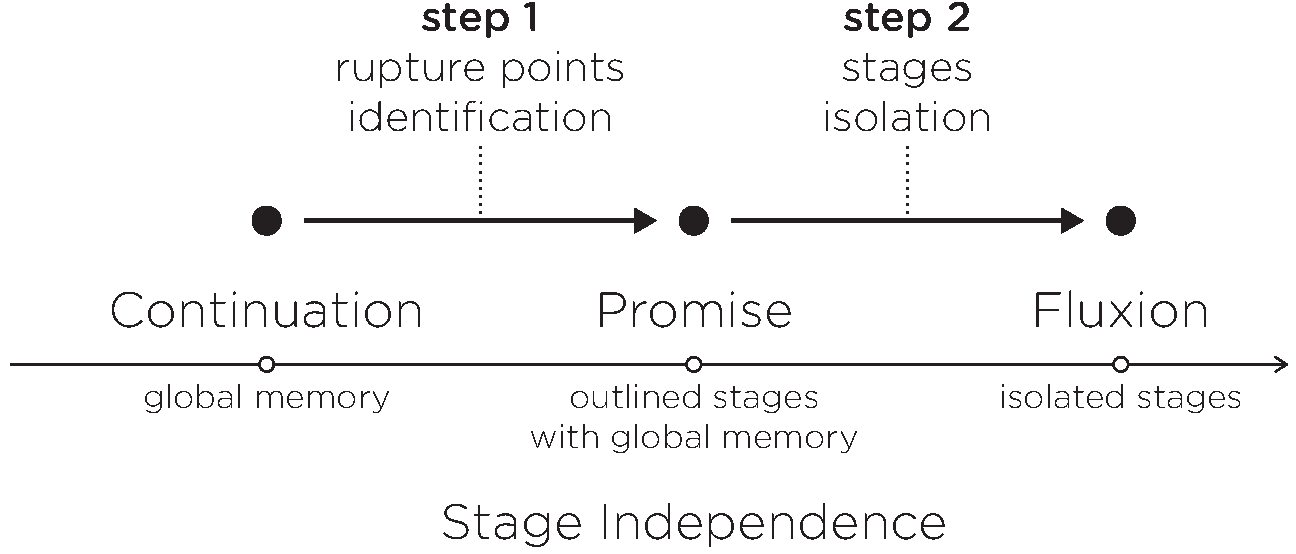
\includegraphics[width=0.7\textwidth]{../resources/roadmap.pdf}%
    \caption{Roadmap}%
    \label{fig:roadmap}%
  }%
\end{figure}

The first compiler focuses on the identification of simple chains of causality between continuations to transform these chains into Promises.
% the transformation from continuations to Promises.
% It focuses on the identification of the chains of causality in continuations.
However, promises are more expressive than the simple chaining of causal sequentiality.
% They force another control over the execution flow.
% According to the outcome of the operation, they call one function to continue the execution with the result, or another to handle errors.
% This conditional execution is indivisible from the Promise specification.
% Promises impose a convention on how to hand back the outcome of the deferred computation, while classic continuations leave this conditional execution to the developer.
Moreover, they impose a different convention than continuations on how to hand back the outcome and errors of the deferred computation.
This difference brings unnecessary complexity to the identification of chains.
To rule out this difference between continuations and Promises, before introducing the first compiler, section \ref{chapter5:due} introduces a simpler specification to Promise, called Due.

The second compiler detects all the chains of causality between continuations and encapsulate them in fluxions.
It isolates the fluxions when possible to allow the parallelism required for efficiency.
This second compilers is introduced in section \ref{chapter5:flx}.

\input{05-implementation/Due/main}
\input{05-implementation/Flx/main}
% \input{05-implementation/Evaluation}

% \subsection{Real test case} \label{chapter5:flx:evaluation}

The compiler is tested on a real application, gifsockets-server\ftnt{https://github.com/twolfson/gifsockets-server}.
This test proves the possibility for an application to be compiled into a network of independent parts.
It shows the current limitations of this isolation and the modifications needed on the application to circumvent them.

\begin{code}[js, caption={Simplified version of gifsockets-server},label={lst:gifsocket}]
var express = require('express'),
    app = express(),
    routes = require('gifsockets-middleware'), //@\label{lst:gifsocket:gif-mw}@
    getRawBody = require('raw-body');

function bodyParser(limit) { //@\label{lst:gifsocket:bodyParser}@
  return function saveBody(req, res, next) { //@\label{lst:gifsocket:saveBody}@
    getRawBody(req, { //@\label{lst:gifsocket:getRawBody}@
      expected: req.headers['content-length'],
      limit: limit
    }, function (err, buffer) { //@\label{lst:gifsocket:callback}@
      req.body = buffer;
      next(); //@\label{lst:gifsocket:next}@
    });
  };
}

app.post('/image/text', bodyParser(1 * 1024 * 1024), routes.writeTextToImages); //@\label{lst:gifsocket:app.post}@
app.listen(8000);
\end{code}

This application, simplified in listing \ref{lst:gifsocket}, is a real-time chat using gif-based communication channels.
It was selected from the evaluation set of the Due compiler because it is simple enough to illustrate this evaluation.
% \cite{Brodu2015}
%  from the \texttt{npm} registry because it depends on \texttt{express}, it is tested, working, and simple enough to illustrate this evaluation.
The server transforms the received text into a gif frame, and pushes it back to a never-ending gif to be displayed on the client.

On line \ref{lst:gifsocket:app.post}, the application registers two functions to process the requests received on the url \texttt{/image/text}.
The closure \texttt{saveBody}, line \ref{lst:gifsocket:saveBody}, returned by \texttt{bodyParser}, line \ref{lst:gifsocket:bodyParser}, and the method \texttt{routes.write\-Text\-To\-Images} from the external module \texttt{gifsockets-\-middleware}, line \ref{lst:gifsocket:gif-mw}.
The closure \texttt{saveBody} calls the asynchronous function \texttt{getRawBody} to get the request body.
Its callback handles the errors, and calls \texttt{next} to continue processing the request with the next function, \texttt{routes.write\-Text\-To\-Images}.

\subsubsection{Compilation} \label{chapter5:flx:evaluation:compilation}

% We compile this application with the compiler
The compilation result is in listing \ref{lst:flx-gifsocket}.
The function call \texttt{app.post}, line \ref{lst:gifsocket:app.post}, is a rupture point.
However, its callbacks, \texttt{bodyParser} and \texttt{routes.write\-Text\-To\-Images} are not declared \textit{in situ}.
They are evaluated as functions only at runtime.
As precised previously, the compiler discards these callbacks to avoid altering the semantic. % by moving or modifying their definition.
% For this reason, the compiler ignores this rupture point, to avoid interfering with the evaluation.

\begin{code}[flx, caption={Compilation result of gifsockets-server},label={lst:flx-gifsocket}]
flx main & express {req}
>> anonymous_1000 [req, next]
  var express = require('express'),
      app = express(),
      routes = require('gifsockets-middleware'), //@\label{lst:flx-gifsocket:gif-mw}@
      getRawBody = require('raw-body');

  function bodyParser(limit) { //@\label{lst:flx-gifsocket:bodyParser}@
    return function saveBody(req, res, next) { //@\label{lst:flx-gifsocket:saveBody}@
      getRawBody(req, { //@\label{lst:flx-gifsocket:getRawBody}@
        expected: req.headers['content-length'], //@\label{lst:flx-gifsocket:req.headers}@
        limit: limit
      }, >> anonymous_1000 [req, next]);
    };
  }

  app.post('/image/text', bodyParser(1 * 1024 * 1024), routes.writeTextToImages); //@\label{lst:flx-gifsocket:app.post}@
  app.listen(8000);

flx anonymous_1000
-> null
  function (err, buffer) { //@\label{lst:flx-gifsocket:callback}@
    req.body = buffer; //@\label{lst:flx-gifsocket:buffer}@
    next(); //@\label{lst:flx-gifsocket:next}@
  }
\end{code}

The compiler detects a rupture point : the function \texttt{get\-Raw\-Body} and its anonymous callback, line \ref{lst:gifsocket:callback}.
It encapsulates this callback in a fluxion named \texttt{anony\-mous\_\-1000}.
The callback is replaced with a stream placeholder to send the message stream to this downstream fluxion.
The variables \texttt{req} and \texttt{next} are appended to this message stream, to propagate their value from the \texttt{main} fluxion to the \texttt{anony\-mous\_\-1000} fluxion.

When \texttt{anony\-mous\_\-1000} is not isolated from the \texttt{main} fluxion, as if they belong to the same group, the compilation result works as expected.
The variables used in the fluxion, \texttt{req} and \texttt{next}, are still shared between the two fluxions.
In this situation fluxions are quite similar to Dues regarding memory shareing.
Our goal is to isolate the two fluxions, to be able to safely parallelize their executions.

\subsubsection{Isolation} \label{chapter5:flx:evaluation:isolation}

In listing \ref{lst:flx-gifsocket}, the fluxion \texttt{anony\-mous\_\-1000} modifies the object \texttt{req}, line \ref{lst:flx-gifsocket:buffer}, to store the text of the received request, and it calls \texttt{next} to continue the execution, line \ref{lst:flx-gifsocket:next}.
\texttt{req} is an alias to a memory location used in multiple palces in code.
Therefore, these operations produce side-effects that should propagate in the whole application, but the isolation prevents this propagation.
Isolating the fluxion \texttt{anony\-mous\_\-1000} produces runtime exceptions.
The next paragraph details how this situation is handled to allow the application to be parallelized.

\paragraph{Variable \texttt{req}}

The variable \texttt{req} is read in fluxion \texttt{main}, lines \ref{lst:flx-gifsocket:getRawBody} and \ref{lst:flx-gifsocket:req.headers}.
Then its property \texttt{body} is associated to \texttt{buffer} in fluxion \texttt{anony\-mous\_\-1000}, line \ref{lst:flx-gifsocket:buffer}.
The compiler is unable to identify the aliases of this variable. % further usages.
However, the side effect resulting from this association impacts a variable in the scope of the next callback, \texttt{routes.write\-Text\-To\-Images}.
In this test case, the application is modified manually to explicitly propagate this side-effect to the next callback through the function \texttt{next}.
The modifications of this function are explained further in the next paragraph.

\paragraph{Closure \texttt{next}}

The function \texttt{next} is a closure provided by the \texttt{express} \texttt{Router} to continue the execution with the next function to handle the client request.
Because it indirectly relies on the variable \texttt{req}, it is impossible to isolate its execution with the \texttt{anony\-mous\_\-1000} fluxion.
Instead, we modify \texttt{express}, so as to be compatible with the fluxional execution model.
We explain the modifications below.

\begin{code}[flx, caption={Simplified modification on the compiled result},label={lst:mflx-gifsocket}]
flx anonymous_1000
-> express_dispatcher
  function (err, buffer) { //@\label{lst:mflx-gifsocket:callback}@
    req.body = buffer; //@\label{lst:mflx-gifsocket:buffer}@
    next_placeholder(req, -> express_dispatcher); //@\label{lst:mflx-gifsocket:next-placeholder}@
  }

flx express_dispatcher & express {req} //@\label{lst:mflx-gifsocket:express-dispatcher}@
-> null
  function (modified_req) {
    merge(req, modified_req);
    next(); //@\label{lst:mflx-gifsocket:next}@
  }
\end{code}

In listing \ref{lst:gifsocket}, the function \texttt{next} is a continuation allowing the anonymous callback, line \ref{lst:gifsocket:callback}, to call the next function to handle the request.
To isolate the anonymous callback into \texttt{anonymous\_\-1000}, \texttt{next} is replaced by a rupture point.
This replacement is illustrated in listing \ref{lst:mflx-gifsocket}.
The \texttt{express} \texttt{Router} registers a fluxion named \texttt{express\_\-dispatcher}, line \ref{lst:mflx-gifsocket:express-dispatcher}, to continue the execution after the fluxion \texttt{anony\-mous\_\-1000}.
This fluxion is in the same group \texttt{express} as the \texttt{main} fluxion, hence it has access to the original variable \texttt{req}, and to the original function \texttt{next}.
The call to the original \texttt{next} function is replaced by a placeholder to push the stream to the fluxion \texttt{express\_\-dispatcher}, line \ref{lst:mflx-gifsocket:next-placeholder}.
The fluxion \texttt{express\_\-dispatcher} receives the stream from the upstream fluxion \texttt{anony\-mous\_\-1000}, merges back the modification in the variable \texttt{req} to propagate the side effects, and finally calls the original function \texttt{next} to continue the execution, line \ref{lst:mflx-gifsocket:next}.

After the modifications detailed above, the server works as expected.
The isolated fluxion correctly receives, and returns its serialized messages.
The client successfully receives a gif frame containing the text.



\subsection{Limitations}

The static analysis used for this compiler presents some limitations.
It is unable to analyze code with dynamic behaviors.
Higher-order programming leads to more productivity partly beacuse it rely on such dynamic behavior to extend expressivity.
Precisely, it allows more levels of indirections.

\subsubsection{Levels of Indirections}

The indirection is an abstraction between the value, and its manipulation.
In listing \ref{lst:indirection}, the variables \texttt{a} and \texttt{b} point both to the same memory object.
The function \texttt{fn} introduces a level of indirection between the real object \texttt{a} and its manipulation handle, \texttt{b};
% Actually, the variable \texttt{a} already introduces a level of indirection between the real object and the handle \texttt{a}.

\begin{code}[js,
  caption={One level of Indirection},
  label={lst:indirection}]
var a = {
      // an object;
    };

fn(b) {
  // modify b;
}

fn(a);
\end{code}

\subsubsection{Uncertainties}

The indirection is trivial to resolve in listing \ref{lst:indirection}.
It only needs to have access to the definition of \texttt{a} and of \texttt{fn}.
%A very simple static analysis could resolve it.
However, in listing \ref{lst:indirections}, the array \texttt{handlers} introduces a new level of indirection.
The static analysis now needs to have access to the definition of \texttt{i} and of the \texttt{handlers}.
If this definition is provided by an external input, it is not available statically, hence, it adds an uncertainty during the analysis. 

\begin{code}[js,
  caption={Two levels of indirection},
  label={lst:indirections}]
var a = {
      // an object;
    },
    handlers = [
      // definition of fn handlers;
    ],
    i = ?;

handlers[i](a);
handlers[i+1](a);
\end{code}

These examples are extremely simplified.
A real application contains enough indirections for the static analysis to be overwhelmed by uncertainties, and to be unable to resolve the variables.
If a variable is left unresolved, it is impossible to assure its scope and its aliases.
Therefore, the compiler is unable to isolate it into a fluxion, or to distribute its modification by messages.

Moreover, it leads the compiler to ignore the rupture points not defined \textit{in situ}, because their modifications could impact the semantic.
The reason for this precaution, is that the compiler is unable to assure where the function is used, and the scope of its variables.
Therefore, it is unable to assure that the modification will conserve the semantic.

\subsubsection{Dynamic Resolution}

In a web application, this variable \texttt{i} might be part of the user request, which is available only at runtime.
It eventually introduces an uncertainty.

This dynamic resolution of variables is precisely what increase expressiveness.
Trying to resolve them statically is equivalent to restrict expressiveness.
No static analysis can overstep these limitations.
Only a dynamic analysis could analysis the resolved indirections during run time to overstep these limitations correctly.




\renewcommand{\glyph}{\iconfont{\XeTeXglyph287}}
\chapter{Implementations} \label{chapter5}
\minitoc
\eject
The transformation allowed by the equivalence from an event-driven program into a distributed network of fluxions is implemented incrementally into two compilers, as presented in figure \ref{fig:roadmap}.
Each compilers is divided into two steps, the identification of the rupture points separating the stages of the pipeline, and the isolation of these stages.
% This chapter presents the technical implementations of these two steps in the transformation from the event-driven execution model to the pipeline architecture
% , the transformation described in the previous chapter was implemented incrementally in two compilers.

\begin{figure}[h!]%
  \textfig{%
    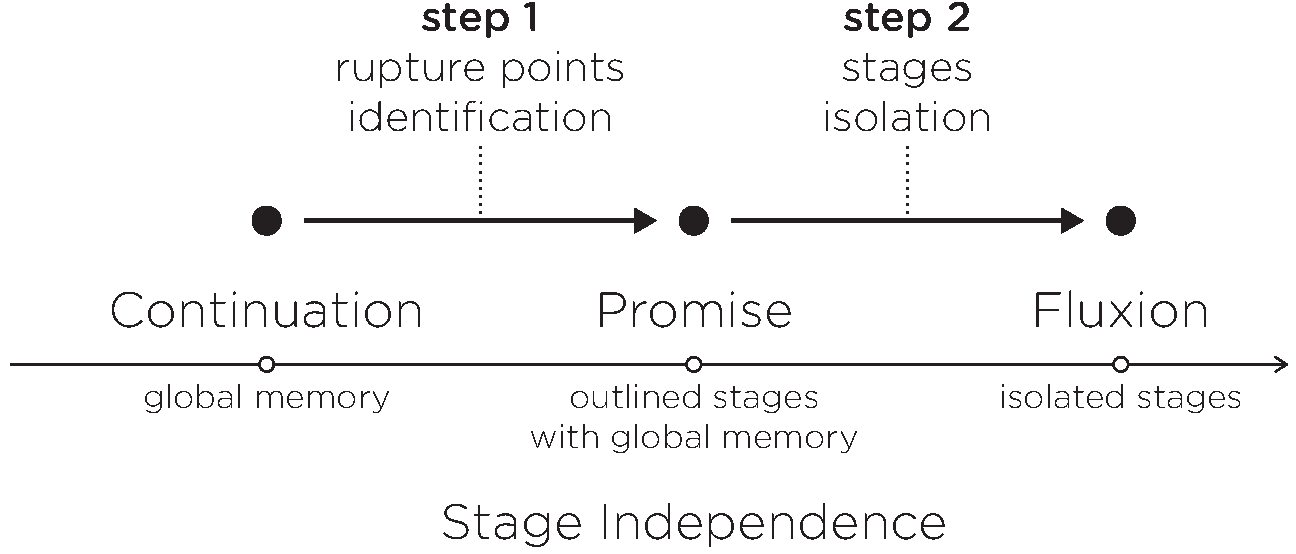
\includegraphics[width=0.7\textwidth]{../resources/roadmap.pdf}%
    \caption{Roadmap}%
    \label{fig:roadmap}%
  }%
\end{figure}

The first compiler focuses on the identification of simple chains of causality between continuations to transform these chains into Promises.
% the transformation from continuations to Promises.
% It focuses on the identification of the chains of causality in continuations.
However, promises are more expressive than the simple chaining of causal sequentiality.
% They force another control over the execution flow.
% According to the outcome of the operation, they call one function to continue the execution with the result, or another to handle errors.
% This conditional execution is indivisible from the Promise specification.
% Promises impose a convention on how to hand back the outcome of the deferred computation, while classic continuations leave this conditional execution to the developer.
Moreover, they impose a different convention than continuations on how to hand back the outcome and errors of the deferred computation.
This difference brings unnecessary complexity to the identification of chains.
To rule out this difference between continuations and Promises, before introducing the first compiler, section \ref{chapter5:due} introduces a simpler specification to Promise, called Due.

The second compiler detects all the chains of causality between continuations and encapsulate them in fluxions.
It isolates the fluxions when possible to allow the parallelism required for efficiency.
This second compilers is introduced in section \ref{chapter5:flx}.

\renewcommand{\glyph}{\iconfont{\XeTeXglyph287}}
\chapter{Implementations} \label{chapter5}
\minitoc
\eject
The transformation allowed by the equivalence from an event-driven program into a distributed network of fluxions is implemented incrementally into two compilers, as presented in figure \ref{fig:roadmap}.
Each compilers is divided into two steps, the identification of the rupture points separating the stages of the pipeline, and the isolation of these stages.
% This chapter presents the technical implementations of these two steps in the transformation from the event-driven execution model to the pipeline architecture
% , the transformation described in the previous chapter was implemented incrementally in two compilers.

\begin{figure}[h!]%
  \textfig{%
    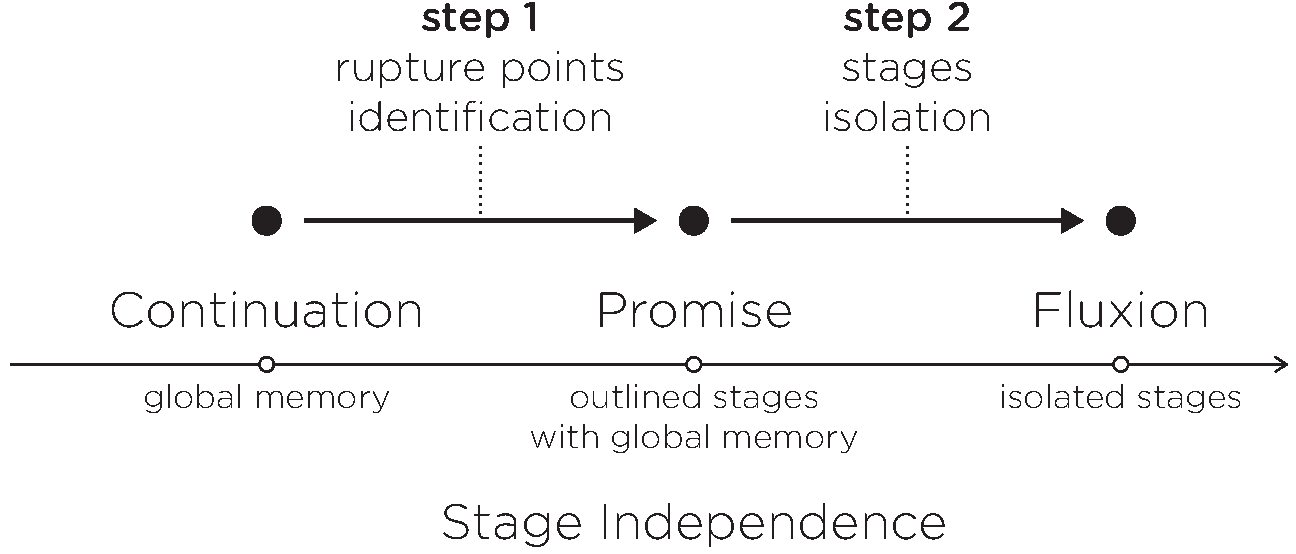
\includegraphics[width=0.7\textwidth]{../resources/roadmap.pdf}%
    \caption{Roadmap}%
    \label{fig:roadmap}%
  }%
\end{figure}

The first compiler focuses on the identification of simple chains of causality between continuations to transform these chains into Promises.
% the transformation from continuations to Promises.
% It focuses on the identification of the chains of causality in continuations.
However, promises are more expressive than the simple chaining of causal sequentiality.
% They force another control over the execution flow.
% According to the outcome of the operation, they call one function to continue the execution with the result, or another to handle errors.
% This conditional execution is indivisible from the Promise specification.
% Promises impose a convention on how to hand back the outcome of the deferred computation, while classic continuations leave this conditional execution to the developer.
Moreover, they impose a different convention than continuations on how to hand back the outcome and errors of the deferred computation.
This difference brings unnecessary complexity to the identification of chains.
To rule out this difference between continuations and Promises, before introducing the first compiler, section \ref{chapter5:due} introduces a simpler specification to Promise, called Due.

The second compiler detects all the chains of causality between continuations and encapsulate them in fluxions.
It isolates the fluxions when possible to allow the parallelism required for efficiency.
This second compilers is introduced in section \ref{chapter5:flx}.

\input{05-implementation/Due/main}
\input{05-implementation/Flx/main}
% \input{05-implementation/Evaluation}

\renewcommand{\glyph}{\iconfont{\XeTeXglyph287}}
\chapter{Implementations} \label{chapter5}
\minitoc
\eject
The transformation allowed by the equivalence from an event-driven program into a distributed network of fluxions is implemented incrementally into two compilers, as presented in figure \ref{fig:roadmap}.
Each compilers is divided into two steps, the identification of the rupture points separating the stages of the pipeline, and the isolation of these stages.
% This chapter presents the technical implementations of these two steps in the transformation from the event-driven execution model to the pipeline architecture
% , the transformation described in the previous chapter was implemented incrementally in two compilers.

\begin{figure}[h!]%
  \textfig{%
    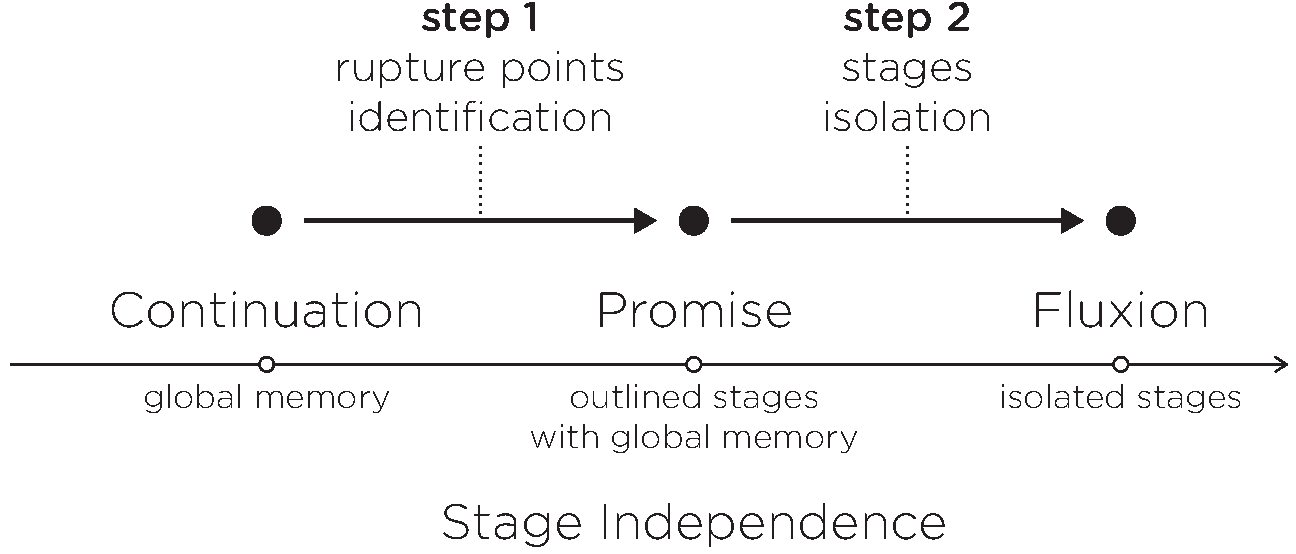
\includegraphics[width=0.7\textwidth]{../resources/roadmap.pdf}%
    \caption{Roadmap}%
    \label{fig:roadmap}%
  }%
\end{figure}

The first compiler focuses on the identification of simple chains of causality between continuations to transform these chains into Promises.
% the transformation from continuations to Promises.
% It focuses on the identification of the chains of causality in continuations.
However, promises are more expressive than the simple chaining of causal sequentiality.
% They force another control over the execution flow.
% According to the outcome of the operation, they call one function to continue the execution with the result, or another to handle errors.
% This conditional execution is indivisible from the Promise specification.
% Promises impose a convention on how to hand back the outcome of the deferred computation, while classic continuations leave this conditional execution to the developer.
Moreover, they impose a different convention than continuations on how to hand back the outcome and errors of the deferred computation.
This difference brings unnecessary complexity to the identification of chains.
To rule out this difference between continuations and Promises, before introducing the first compiler, section \ref{chapter5:due} introduces a simpler specification to Promise, called Due.

The second compiler detects all the chains of causality between continuations and encapsulate them in fluxions.
It isolates the fluxions when possible to allow the parallelism required for efficiency.
This second compilers is introduced in section \ref{chapter5:flx}.

\input{05-implementation/Due/main}
\input{05-implementation/Flx/main}
% \input{05-implementation/Evaluation}

% \subsection{Real test case} \label{chapter5:flx:evaluation}

The compiler is tested on a real application, gifsockets-server\ftnt{https://github.com/twolfson/gifsockets-server}.
This test proves the possibility for an application to be compiled into a network of independent parts.
It shows the current limitations of this isolation and the modifications needed on the application to circumvent them.

\begin{code}[js, caption={Simplified version of gifsockets-server},label={lst:gifsocket}]
var express = require('express'),
    app = express(),
    routes = require('gifsockets-middleware'), //@\label{lst:gifsocket:gif-mw}@
    getRawBody = require('raw-body');

function bodyParser(limit) { //@\label{lst:gifsocket:bodyParser}@
  return function saveBody(req, res, next) { //@\label{lst:gifsocket:saveBody}@
    getRawBody(req, { //@\label{lst:gifsocket:getRawBody}@
      expected: req.headers['content-length'],
      limit: limit
    }, function (err, buffer) { //@\label{lst:gifsocket:callback}@
      req.body = buffer;
      next(); //@\label{lst:gifsocket:next}@
    });
  };
}

app.post('/image/text', bodyParser(1 * 1024 * 1024), routes.writeTextToImages); //@\label{lst:gifsocket:app.post}@
app.listen(8000);
\end{code}

This application, simplified in listing \ref{lst:gifsocket}, is a real-time chat using gif-based communication channels.
It was selected from the evaluation set of the Due compiler because it is simple enough to illustrate this evaluation.
% \cite{Brodu2015}
%  from the \texttt{npm} registry because it depends on \texttt{express}, it is tested, working, and simple enough to illustrate this evaluation.
The server transforms the received text into a gif frame, and pushes it back to a never-ending gif to be displayed on the client.

On line \ref{lst:gifsocket:app.post}, the application registers two functions to process the requests received on the url \texttt{/image/text}.
The closure \texttt{saveBody}, line \ref{lst:gifsocket:saveBody}, returned by \texttt{bodyParser}, line \ref{lst:gifsocket:bodyParser}, and the method \texttt{routes.write\-Text\-To\-Images} from the external module \texttt{gifsockets-\-middleware}, line \ref{lst:gifsocket:gif-mw}.
The closure \texttt{saveBody} calls the asynchronous function \texttt{getRawBody} to get the request body.
Its callback handles the errors, and calls \texttt{next} to continue processing the request with the next function, \texttt{routes.write\-Text\-To\-Images}.

\subsubsection{Compilation} \label{chapter5:flx:evaluation:compilation}

% We compile this application with the compiler
The compilation result is in listing \ref{lst:flx-gifsocket}.
The function call \texttt{app.post}, line \ref{lst:gifsocket:app.post}, is a rupture point.
However, its callbacks, \texttt{bodyParser} and \texttt{routes.write\-Text\-To\-Images} are not declared \textit{in situ}.
They are evaluated as functions only at runtime.
As precised previously, the compiler discards these callbacks to avoid altering the semantic. % by moving or modifying their definition.
% For this reason, the compiler ignores this rupture point, to avoid interfering with the evaluation.

\begin{code}[flx, caption={Compilation result of gifsockets-server},label={lst:flx-gifsocket}]
flx main & express {req}
>> anonymous_1000 [req, next]
  var express = require('express'),
      app = express(),
      routes = require('gifsockets-middleware'), //@\label{lst:flx-gifsocket:gif-mw}@
      getRawBody = require('raw-body');

  function bodyParser(limit) { //@\label{lst:flx-gifsocket:bodyParser}@
    return function saveBody(req, res, next) { //@\label{lst:flx-gifsocket:saveBody}@
      getRawBody(req, { //@\label{lst:flx-gifsocket:getRawBody}@
        expected: req.headers['content-length'], //@\label{lst:flx-gifsocket:req.headers}@
        limit: limit
      }, >> anonymous_1000 [req, next]);
    };
  }

  app.post('/image/text', bodyParser(1 * 1024 * 1024), routes.writeTextToImages); //@\label{lst:flx-gifsocket:app.post}@
  app.listen(8000);

flx anonymous_1000
-> null
  function (err, buffer) { //@\label{lst:flx-gifsocket:callback}@
    req.body = buffer; //@\label{lst:flx-gifsocket:buffer}@
    next(); //@\label{lst:flx-gifsocket:next}@
  }
\end{code}

The compiler detects a rupture point : the function \texttt{get\-Raw\-Body} and its anonymous callback, line \ref{lst:gifsocket:callback}.
It encapsulates this callback in a fluxion named \texttt{anony\-mous\_\-1000}.
The callback is replaced with a stream placeholder to send the message stream to this downstream fluxion.
The variables \texttt{req} and \texttt{next} are appended to this message stream, to propagate their value from the \texttt{main} fluxion to the \texttt{anony\-mous\_\-1000} fluxion.

When \texttt{anony\-mous\_\-1000} is not isolated from the \texttt{main} fluxion, as if they belong to the same group, the compilation result works as expected.
The variables used in the fluxion, \texttt{req} and \texttt{next}, are still shared between the two fluxions.
In this situation fluxions are quite similar to Dues regarding memory shareing.
Our goal is to isolate the two fluxions, to be able to safely parallelize their executions.

\subsubsection{Isolation} \label{chapter5:flx:evaluation:isolation}

In listing \ref{lst:flx-gifsocket}, the fluxion \texttt{anony\-mous\_\-1000} modifies the object \texttt{req}, line \ref{lst:flx-gifsocket:buffer}, to store the text of the received request, and it calls \texttt{next} to continue the execution, line \ref{lst:flx-gifsocket:next}.
\texttt{req} is an alias to a memory location used in multiple palces in code.
Therefore, these operations produce side-effects that should propagate in the whole application, but the isolation prevents this propagation.
Isolating the fluxion \texttt{anony\-mous\_\-1000} produces runtime exceptions.
The next paragraph details how this situation is handled to allow the application to be parallelized.

\paragraph{Variable \texttt{req}}

The variable \texttt{req} is read in fluxion \texttt{main}, lines \ref{lst:flx-gifsocket:getRawBody} and \ref{lst:flx-gifsocket:req.headers}.
Then its property \texttt{body} is associated to \texttt{buffer} in fluxion \texttt{anony\-mous\_\-1000}, line \ref{lst:flx-gifsocket:buffer}.
The compiler is unable to identify the aliases of this variable. % further usages.
However, the side effect resulting from this association impacts a variable in the scope of the next callback, \texttt{routes.write\-Text\-To\-Images}.
In this test case, the application is modified manually to explicitly propagate this side-effect to the next callback through the function \texttt{next}.
The modifications of this function are explained further in the next paragraph.

\paragraph{Closure \texttt{next}}

The function \texttt{next} is a closure provided by the \texttt{express} \texttt{Router} to continue the execution with the next function to handle the client request.
Because it indirectly relies on the variable \texttt{req}, it is impossible to isolate its execution with the \texttt{anony\-mous\_\-1000} fluxion.
Instead, we modify \texttt{express}, so as to be compatible with the fluxional execution model.
We explain the modifications below.

\begin{code}[flx, caption={Simplified modification on the compiled result},label={lst:mflx-gifsocket}]
flx anonymous_1000
-> express_dispatcher
  function (err, buffer) { //@\label{lst:mflx-gifsocket:callback}@
    req.body = buffer; //@\label{lst:mflx-gifsocket:buffer}@
    next_placeholder(req, -> express_dispatcher); //@\label{lst:mflx-gifsocket:next-placeholder}@
  }

flx express_dispatcher & express {req} //@\label{lst:mflx-gifsocket:express-dispatcher}@
-> null
  function (modified_req) {
    merge(req, modified_req);
    next(); //@\label{lst:mflx-gifsocket:next}@
  }
\end{code}

In listing \ref{lst:gifsocket}, the function \texttt{next} is a continuation allowing the anonymous callback, line \ref{lst:gifsocket:callback}, to call the next function to handle the request.
To isolate the anonymous callback into \texttt{anonymous\_\-1000}, \texttt{next} is replaced by a rupture point.
This replacement is illustrated in listing \ref{lst:mflx-gifsocket}.
The \texttt{express} \texttt{Router} registers a fluxion named \texttt{express\_\-dispatcher}, line \ref{lst:mflx-gifsocket:express-dispatcher}, to continue the execution after the fluxion \texttt{anony\-mous\_\-1000}.
This fluxion is in the same group \texttt{express} as the \texttt{main} fluxion, hence it has access to the original variable \texttt{req}, and to the original function \texttt{next}.
The call to the original \texttt{next} function is replaced by a placeholder to push the stream to the fluxion \texttt{express\_\-dispatcher}, line \ref{lst:mflx-gifsocket:next-placeholder}.
The fluxion \texttt{express\_\-dispatcher} receives the stream from the upstream fluxion \texttt{anony\-mous\_\-1000}, merges back the modification in the variable \texttt{req} to propagate the side effects, and finally calls the original function \texttt{next} to continue the execution, line \ref{lst:mflx-gifsocket:next}.

After the modifications detailed above, the server works as expected.
The isolated fluxion correctly receives, and returns its serialized messages.
The client successfully receives a gif frame containing the text.



\subsection{Limitations}

The static analysis used for this compiler presents some limitations.
It is unable to analyze code with dynamic behaviors.
Higher-order programming leads to more productivity partly beacuse it rely on such dynamic behavior to extend expressivity.
Precisely, it allows more levels of indirections.

\subsubsection{Levels of Indirections}

The indirection is an abstraction between the value, and its manipulation.
In listing \ref{lst:indirection}, the variables \texttt{a} and \texttt{b} point both to the same memory object.
The function \texttt{fn} introduces a level of indirection between the real object \texttt{a} and its manipulation handle, \texttt{b};
% Actually, the variable \texttt{a} already introduces a level of indirection between the real object and the handle \texttt{a}.

\begin{code}[js,
  caption={One level of Indirection},
  label={lst:indirection}]
var a = {
      // an object;
    };

fn(b) {
  // modify b;
}

fn(a);
\end{code}

\subsubsection{Uncertainties}

The indirection is trivial to resolve in listing \ref{lst:indirection}.
It only needs to have access to the definition of \texttt{a} and of \texttt{fn}.
%A very simple static analysis could resolve it.
However, in listing \ref{lst:indirections}, the array \texttt{handlers} introduces a new level of indirection.
The static analysis now needs to have access to the definition of \texttt{i} and of the \texttt{handlers}.
If this definition is provided by an external input, it is not available statically, hence, it adds an uncertainty during the analysis. 

\begin{code}[js,
  caption={Two levels of indirection},
  label={lst:indirections}]
var a = {
      // an object;
    },
    handlers = [
      // definition of fn handlers;
    ],
    i = ?;

handlers[i](a);
handlers[i+1](a);
\end{code}

These examples are extremely simplified.
A real application contains enough indirections for the static analysis to be overwhelmed by uncertainties, and to be unable to resolve the variables.
If a variable is left unresolved, it is impossible to assure its scope and its aliases.
Therefore, the compiler is unable to isolate it into a fluxion, or to distribute its modification by messages.

Moreover, it leads the compiler to ignore the rupture points not defined \textit{in situ}, because their modifications could impact the semantic.
The reason for this precaution, is that the compiler is unable to assure where the function is used, and the scope of its variables.
Therefore, it is unable to assure that the modification will conserve the semantic.

\subsubsection{Dynamic Resolution}

In a web application, this variable \texttt{i} might be part of the user request, which is available only at runtime.
It eventually introduces an uncertainty.

This dynamic resolution of variables is precisely what increase expressiveness.
Trying to resolve them statically is equivalent to restrict expressiveness.
No static analysis can overstep these limitations.
Only a dynamic analysis could analysis the resolved indirections during run time to overstep these limitations correctly.




% \subsection{Real test case} \label{chapter5:flx:evaluation}

The compiler is tested on a real application, gifsockets-server\ftnt{https://github.com/twolfson/gifsockets-server}.
This test proves the possibility for an application to be compiled into a network of independent parts.
It shows the current limitations of this isolation and the modifications needed on the application to circumvent them.

\begin{code}[js, caption={Simplified version of gifsockets-server},label={lst:gifsocket}]
var express = require('express'),
    app = express(),
    routes = require('gifsockets-middleware'), //@\label{lst:gifsocket:gif-mw}@
    getRawBody = require('raw-body');

function bodyParser(limit) { //@\label{lst:gifsocket:bodyParser}@
  return function saveBody(req, res, next) { //@\label{lst:gifsocket:saveBody}@
    getRawBody(req, { //@\label{lst:gifsocket:getRawBody}@
      expected: req.headers['content-length'],
      limit: limit
    }, function (err, buffer) { //@\label{lst:gifsocket:callback}@
      req.body = buffer;
      next(); //@\label{lst:gifsocket:next}@
    });
  };
}

app.post('/image/text', bodyParser(1 * 1024 * 1024), routes.writeTextToImages); //@\label{lst:gifsocket:app.post}@
app.listen(8000);
\end{code}

This application, simplified in listing \ref{lst:gifsocket}, is a real-time chat using gif-based communication channels.
It was selected from the evaluation set of the Due compiler because it is simple enough to illustrate this evaluation.
% \cite{Brodu2015}
%  from the \texttt{npm} registry because it depends on \texttt{express}, it is tested, working, and simple enough to illustrate this evaluation.
The server transforms the received text into a gif frame, and pushes it back to a never-ending gif to be displayed on the client.

On line \ref{lst:gifsocket:app.post}, the application registers two functions to process the requests received on the url \texttt{/image/text}.
The closure \texttt{saveBody}, line \ref{lst:gifsocket:saveBody}, returned by \texttt{bodyParser}, line \ref{lst:gifsocket:bodyParser}, and the method \texttt{routes.write\-Text\-To\-Images} from the external module \texttt{gifsockets-\-middleware}, line \ref{lst:gifsocket:gif-mw}.
The closure \texttt{saveBody} calls the asynchronous function \texttt{getRawBody} to get the request body.
Its callback handles the errors, and calls \texttt{next} to continue processing the request with the next function, \texttt{routes.write\-Text\-To\-Images}.

\subsubsection{Compilation} \label{chapter5:flx:evaluation:compilation}

% We compile this application with the compiler
The compilation result is in listing \ref{lst:flx-gifsocket}.
The function call \texttt{app.post}, line \ref{lst:gifsocket:app.post}, is a rupture point.
However, its callbacks, \texttt{bodyParser} and \texttt{routes.write\-Text\-To\-Images} are not declared \textit{in situ}.
They are evaluated as functions only at runtime.
As precised previously, the compiler discards these callbacks to avoid altering the semantic. % by moving or modifying their definition.
% For this reason, the compiler ignores this rupture point, to avoid interfering with the evaluation.

\begin{code}[flx, caption={Compilation result of gifsockets-server},label={lst:flx-gifsocket}]
flx main & express {req}
>> anonymous_1000 [req, next]
  var express = require('express'),
      app = express(),
      routes = require('gifsockets-middleware'), //@\label{lst:flx-gifsocket:gif-mw}@
      getRawBody = require('raw-body');

  function bodyParser(limit) { //@\label{lst:flx-gifsocket:bodyParser}@
    return function saveBody(req, res, next) { //@\label{lst:flx-gifsocket:saveBody}@
      getRawBody(req, { //@\label{lst:flx-gifsocket:getRawBody}@
        expected: req.headers['content-length'], //@\label{lst:flx-gifsocket:req.headers}@
        limit: limit
      }, >> anonymous_1000 [req, next]);
    };
  }

  app.post('/image/text', bodyParser(1 * 1024 * 1024), routes.writeTextToImages); //@\label{lst:flx-gifsocket:app.post}@
  app.listen(8000);

flx anonymous_1000
-> null
  function (err, buffer) { //@\label{lst:flx-gifsocket:callback}@
    req.body = buffer; //@\label{lst:flx-gifsocket:buffer}@
    next(); //@\label{lst:flx-gifsocket:next}@
  }
\end{code}

The compiler detects a rupture point : the function \texttt{get\-Raw\-Body} and its anonymous callback, line \ref{lst:gifsocket:callback}.
It encapsulates this callback in a fluxion named \texttt{anony\-mous\_\-1000}.
The callback is replaced with a stream placeholder to send the message stream to this downstream fluxion.
The variables \texttt{req} and \texttt{next} are appended to this message stream, to propagate their value from the \texttt{main} fluxion to the \texttt{anony\-mous\_\-1000} fluxion.

When \texttt{anony\-mous\_\-1000} is not isolated from the \texttt{main} fluxion, as if they belong to the same group, the compilation result works as expected.
The variables used in the fluxion, \texttt{req} and \texttt{next}, are still shared between the two fluxions.
In this situation fluxions are quite similar to Dues regarding memory shareing.
Our goal is to isolate the two fluxions, to be able to safely parallelize their executions.

\subsubsection{Isolation} \label{chapter5:flx:evaluation:isolation}

In listing \ref{lst:flx-gifsocket}, the fluxion \texttt{anony\-mous\_\-1000} modifies the object \texttt{req}, line \ref{lst:flx-gifsocket:buffer}, to store the text of the received request, and it calls \texttt{next} to continue the execution, line \ref{lst:flx-gifsocket:next}.
\texttt{req} is an alias to a memory location used in multiple palces in code.
Therefore, these operations produce side-effects that should propagate in the whole application, but the isolation prevents this propagation.
Isolating the fluxion \texttt{anony\-mous\_\-1000} produces runtime exceptions.
The next paragraph details how this situation is handled to allow the application to be parallelized.

\paragraph{Variable \texttt{req}}

The variable \texttt{req} is read in fluxion \texttt{main}, lines \ref{lst:flx-gifsocket:getRawBody} and \ref{lst:flx-gifsocket:req.headers}.
Then its property \texttt{body} is associated to \texttt{buffer} in fluxion \texttt{anony\-mous\_\-1000}, line \ref{lst:flx-gifsocket:buffer}.
The compiler is unable to identify the aliases of this variable. % further usages.
However, the side effect resulting from this association impacts a variable in the scope of the next callback, \texttt{routes.write\-Text\-To\-Images}.
In this test case, the application is modified manually to explicitly propagate this side-effect to the next callback through the function \texttt{next}.
The modifications of this function are explained further in the next paragraph.

\paragraph{Closure \texttt{next}}

The function \texttt{next} is a closure provided by the \texttt{express} \texttt{Router} to continue the execution with the next function to handle the client request.
Because it indirectly relies on the variable \texttt{req}, it is impossible to isolate its execution with the \texttt{anony\-mous\_\-1000} fluxion.
Instead, we modify \texttt{express}, so as to be compatible with the fluxional execution model.
We explain the modifications below.

\begin{code}[flx, caption={Simplified modification on the compiled result},label={lst:mflx-gifsocket}]
flx anonymous_1000
-> express_dispatcher
  function (err, buffer) { //@\label{lst:mflx-gifsocket:callback}@
    req.body = buffer; //@\label{lst:mflx-gifsocket:buffer}@
    next_placeholder(req, -> express_dispatcher); //@\label{lst:mflx-gifsocket:next-placeholder}@
  }

flx express_dispatcher & express {req} //@\label{lst:mflx-gifsocket:express-dispatcher}@
-> null
  function (modified_req) {
    merge(req, modified_req);
    next(); //@\label{lst:mflx-gifsocket:next}@
  }
\end{code}

In listing \ref{lst:gifsocket}, the function \texttt{next} is a continuation allowing the anonymous callback, line \ref{lst:gifsocket:callback}, to call the next function to handle the request.
To isolate the anonymous callback into \texttt{anonymous\_\-1000}, \texttt{next} is replaced by a rupture point.
This replacement is illustrated in listing \ref{lst:mflx-gifsocket}.
The \texttt{express} \texttt{Router} registers a fluxion named \texttt{express\_\-dispatcher}, line \ref{lst:mflx-gifsocket:express-dispatcher}, to continue the execution after the fluxion \texttt{anony\-mous\_\-1000}.
This fluxion is in the same group \texttt{express} as the \texttt{main} fluxion, hence it has access to the original variable \texttt{req}, and to the original function \texttt{next}.
The call to the original \texttt{next} function is replaced by a placeholder to push the stream to the fluxion \texttt{express\_\-dispatcher}, line \ref{lst:mflx-gifsocket:next-placeholder}.
The fluxion \texttt{express\_\-dispatcher} receives the stream from the upstream fluxion \texttt{anony\-mous\_\-1000}, merges back the modification in the variable \texttt{req} to propagate the side effects, and finally calls the original function \texttt{next} to continue the execution, line \ref{lst:mflx-gifsocket:next}.

After the modifications detailed above, the server works as expected.
The isolated fluxion correctly receives, and returns its serialized messages.
The client successfully receives a gif frame containing the text.



\subsection{Limitations}

The static analysis used for this compiler presents some limitations.
It is unable to analyze code with dynamic behaviors.
Higher-order programming leads to more productivity partly beacuse it rely on such dynamic behavior to extend expressivity.
Precisely, it allows more levels of indirections.

\subsubsection{Levels of Indirections}

The indirection is an abstraction between the value, and its manipulation.
In listing \ref{lst:indirection}, the variables \texttt{a} and \texttt{b} point both to the same memory object.
The function \texttt{fn} introduces a level of indirection between the real object \texttt{a} and its manipulation handle, \texttt{b};
% Actually, the variable \texttt{a} already introduces a level of indirection between the real object and the handle \texttt{a}.

\begin{code}[js,
  caption={One level of Indirection},
  label={lst:indirection}]
var a = {
      // an object;
    };

fn(b) {
  // modify b;
}

fn(a);
\end{code}

\subsubsection{Uncertainties}

The indirection is trivial to resolve in listing \ref{lst:indirection}.
It only needs to have access to the definition of \texttt{a} and of \texttt{fn}.
%A very simple static analysis could resolve it.
However, in listing \ref{lst:indirections}, the array \texttt{handlers} introduces a new level of indirection.
The static analysis now needs to have access to the definition of \texttt{i} and of the \texttt{handlers}.
If this definition is provided by an external input, it is not available statically, hence, it adds an uncertainty during the analysis. 

\begin{code}[js,
  caption={Two levels of indirection},
  label={lst:indirections}]
var a = {
      // an object;
    },
    handlers = [
      // definition of fn handlers;
    ],
    i = ?;

handlers[i](a);
handlers[i+1](a);
\end{code}

These examples are extremely simplified.
A real application contains enough indirections for the static analysis to be overwhelmed by uncertainties, and to be unable to resolve the variables.
If a variable is left unresolved, it is impossible to assure its scope and its aliases.
Therefore, the compiler is unable to isolate it into a fluxion, or to distribute its modification by messages.

Moreover, it leads the compiler to ignore the rupture points not defined \textit{in situ}, because their modifications could impact the semantic.
The reason for this precaution, is that the compiler is unable to assure where the function is used, and the scope of its variables.
Therefore, it is unable to assure that the modification will conserve the semantic.

\subsubsection{Dynamic Resolution}

In a web application, this variable \texttt{i} might be part of the user request, which is available only at runtime.
It eventually introduces an uncertainty.

This dynamic resolution of variables is precisely what increase expressiveness.
Trying to resolve them statically is equivalent to restrict expressiveness.
No static analysis can overstep these limitations.
Only a dynamic analysis could analysis the resolved indirections during run time to overstep these limitations correctly.





\chapter{A framework for parallel web applications}
  \section{Fluxions}

\chapter{A compiler toward parallel web application}
  \section{Callback Identification}
    \subsection{Dues}
    \subsection{\comment{TODO}}
  \section{Callback Isolation}
    \subsection{Scope identification}
      \subsubsection{Scope leaking}
    \subsection{Execution propagation}

\chapter{Evaluation}

\renewcommand{\glyph}{\iconfont{\XeTeXglyph287}}
\chapter{Implementations} \label{chapter5}
\minitoc
\eject
The transformation allowed by the equivalence from an event-driven program into a distributed network of fluxions is implemented incrementally into two compilers, as presented in figure \ref{fig:roadmap}.
Each compilers is divided into two steps, the identification of the rupture points separating the stages of the pipeline, and the isolation of these stages.
% This chapter presents the technical implementations of these two steps in the transformation from the event-driven execution model to the pipeline architecture
% , the transformation described in the previous chapter was implemented incrementally in two compilers.

\begin{figure}[h!]%
  \textfig{%
    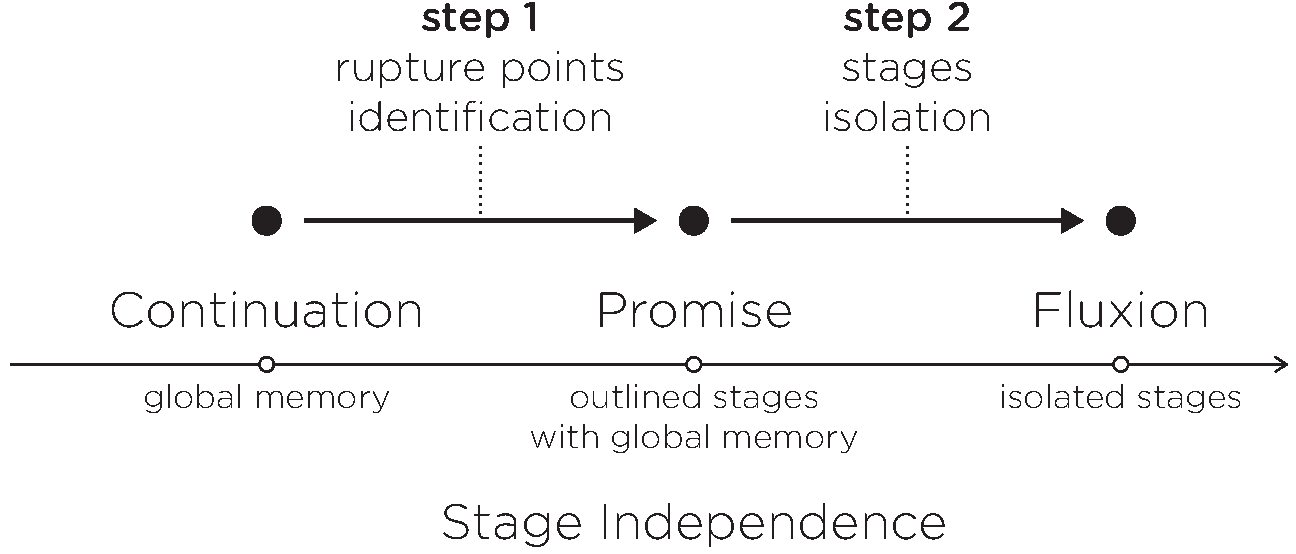
\includegraphics[width=0.7\textwidth]{../resources/roadmap.pdf}%
    \caption{Roadmap}%
    \label{fig:roadmap}%
  }%
\end{figure}

The first compiler focuses on the identification of simple chains of causality between continuations to transform these chains into Promises.
% the transformation from continuations to Promises.
% It focuses on the identification of the chains of causality in continuations.
However, promises are more expressive than the simple chaining of causal sequentiality.
% They force another control over the execution flow.
% According to the outcome of the operation, they call one function to continue the execution with the result, or another to handle errors.
% This conditional execution is indivisible from the Promise specification.
% Promises impose a convention on how to hand back the outcome of the deferred computation, while classic continuations leave this conditional execution to the developer.
Moreover, they impose a different convention than continuations on how to hand back the outcome and errors of the deferred computation.
This difference brings unnecessary complexity to the identification of chains.
To rule out this difference between continuations and Promises, before introducing the first compiler, section \ref{chapter5:due} introduces a simpler specification to Promise, called Due.

The second compiler detects all the chains of causality between continuations and encapsulate them in fluxions.
It isolates the fluxions when possible to allow the parallelism required for efficiency.
This second compilers is introduced in section \ref{chapter5:flx}.

\renewcommand{\glyph}{\iconfont{\XeTeXglyph287}}
\chapter{Implementations} \label{chapter5}
\minitoc
\eject
The transformation allowed by the equivalence from an event-driven program into a distributed network of fluxions is implemented incrementally into two compilers, as presented in figure \ref{fig:roadmap}.
Each compilers is divided into two steps, the identification of the rupture points separating the stages of the pipeline, and the isolation of these stages.
% This chapter presents the technical implementations of these two steps in the transformation from the event-driven execution model to the pipeline architecture
% , the transformation described in the previous chapter was implemented incrementally in two compilers.

\begin{figure}[h!]%
  \textfig{%
    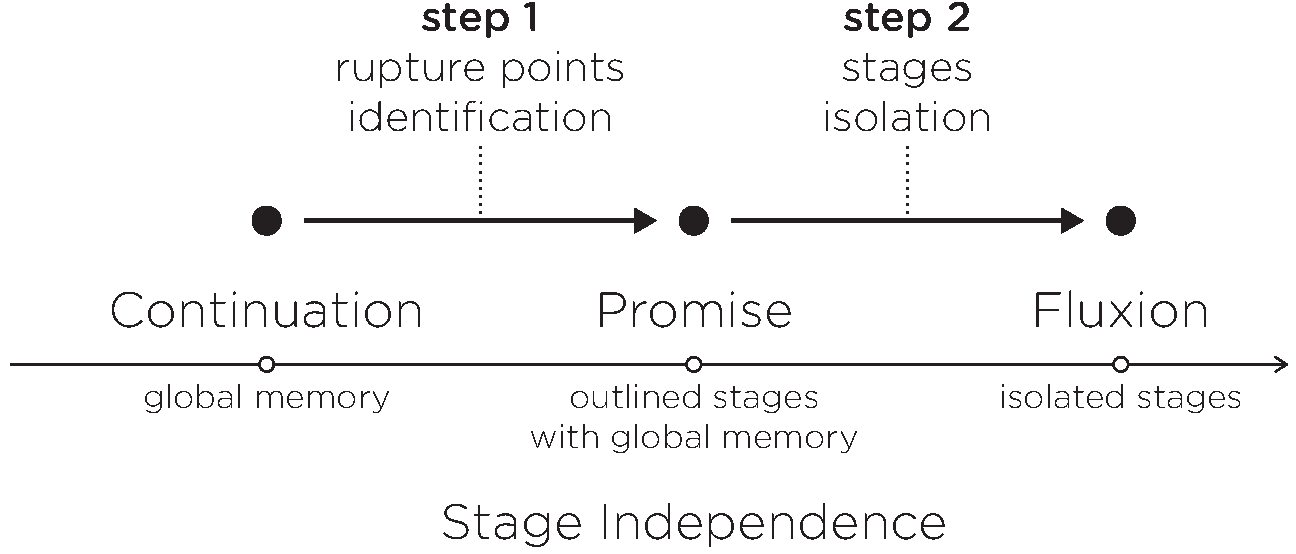
\includegraphics[width=0.7\textwidth]{../resources/roadmap.pdf}%
    \caption{Roadmap}%
    \label{fig:roadmap}%
  }%
\end{figure}

The first compiler focuses on the identification of simple chains of causality between continuations to transform these chains into Promises.
% the transformation from continuations to Promises.
% It focuses on the identification of the chains of causality in continuations.
However, promises are more expressive than the simple chaining of causal sequentiality.
% They force another control over the execution flow.
% According to the outcome of the operation, they call one function to continue the execution with the result, or another to handle errors.
% This conditional execution is indivisible from the Promise specification.
% Promises impose a convention on how to hand back the outcome of the deferred computation, while classic continuations leave this conditional execution to the developer.
Moreover, they impose a different convention than continuations on how to hand back the outcome and errors of the deferred computation.
This difference brings unnecessary complexity to the identification of chains.
To rule out this difference between continuations and Promises, before introducing the first compiler, section \ref{chapter5:due} introduces a simpler specification to Promise, called Due.

The second compiler detects all the chains of causality between continuations and encapsulate them in fluxions.
It isolates the fluxions when possible to allow the parallelism required for efficiency.
This second compilers is introduced in section \ref{chapter5:flx}.

\renewcommand{\glyph}{\iconfont{\XeTeXglyph287}}
\chapter{Implementations} \label{chapter5}
\minitoc
\eject
The transformation allowed by the equivalence from an event-driven program into a distributed network of fluxions is implemented incrementally into two compilers, as presented in figure \ref{fig:roadmap}.
Each compilers is divided into two steps, the identification of the rupture points separating the stages of the pipeline, and the isolation of these stages.
% This chapter presents the technical implementations of these two steps in the transformation from the event-driven execution model to the pipeline architecture
% , the transformation described in the previous chapter was implemented incrementally in two compilers.

\begin{figure}[h!]%
  \textfig{%
    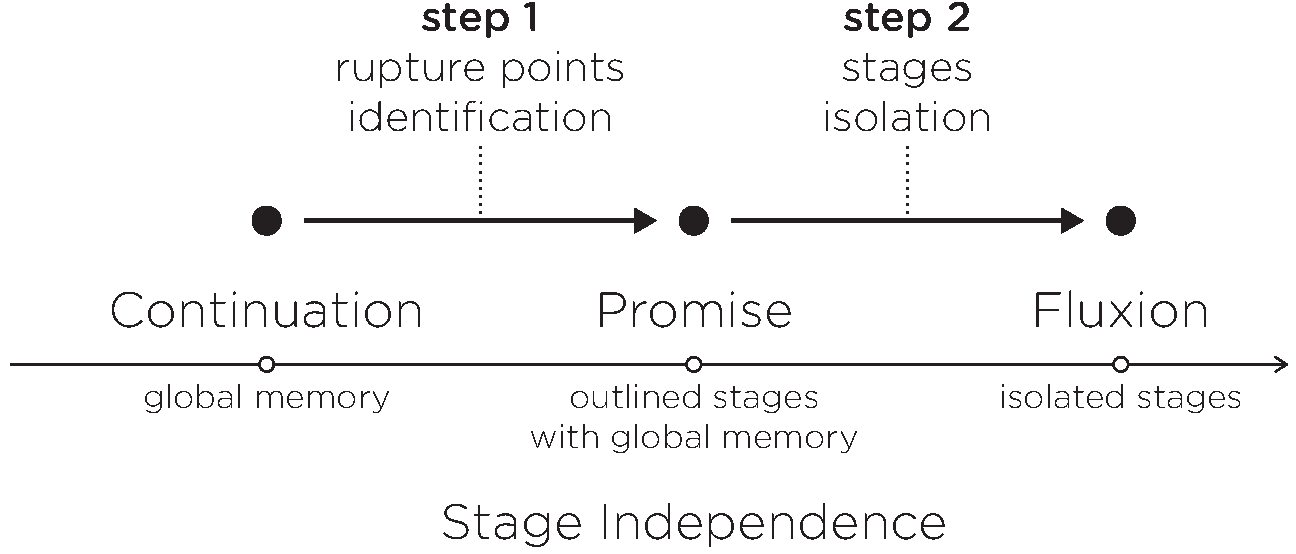
\includegraphics[width=0.7\textwidth]{../resources/roadmap.pdf}%
    \caption{Roadmap}%
    \label{fig:roadmap}%
  }%
\end{figure}

The first compiler focuses on the identification of simple chains of causality between continuations to transform these chains into Promises.
% the transformation from continuations to Promises.
% It focuses on the identification of the chains of causality in continuations.
However, promises are more expressive than the simple chaining of causal sequentiality.
% They force another control over the execution flow.
% According to the outcome of the operation, they call one function to continue the execution with the result, or another to handle errors.
% This conditional execution is indivisible from the Promise specification.
% Promises impose a convention on how to hand back the outcome of the deferred computation, while classic continuations leave this conditional execution to the developer.
Moreover, they impose a different convention than continuations on how to hand back the outcome and errors of the deferred computation.
This difference brings unnecessary complexity to the identification of chains.
To rule out this difference between continuations and Promises, before introducing the first compiler, section \ref{chapter5:due} introduces a simpler specification to Promise, called Due.

The second compiler detects all the chains of causality between continuations and encapsulate them in fluxions.
It isolates the fluxions when possible to allow the parallelism required for efficiency.
This second compilers is introduced in section \ref{chapter5:flx}.

\input{05-implementation/Due/main}
\input{05-implementation/Flx/main}
% \input{05-implementation/Evaluation}

\renewcommand{\glyph}{\iconfont{\XeTeXglyph287}}
\chapter{Implementations} \label{chapter5}
\minitoc
\eject
The transformation allowed by the equivalence from an event-driven program into a distributed network of fluxions is implemented incrementally into two compilers, as presented in figure \ref{fig:roadmap}.
Each compilers is divided into two steps, the identification of the rupture points separating the stages of the pipeline, and the isolation of these stages.
% This chapter presents the technical implementations of these two steps in the transformation from the event-driven execution model to the pipeline architecture
% , the transformation described in the previous chapter was implemented incrementally in two compilers.

\begin{figure}[h!]%
  \textfig{%
    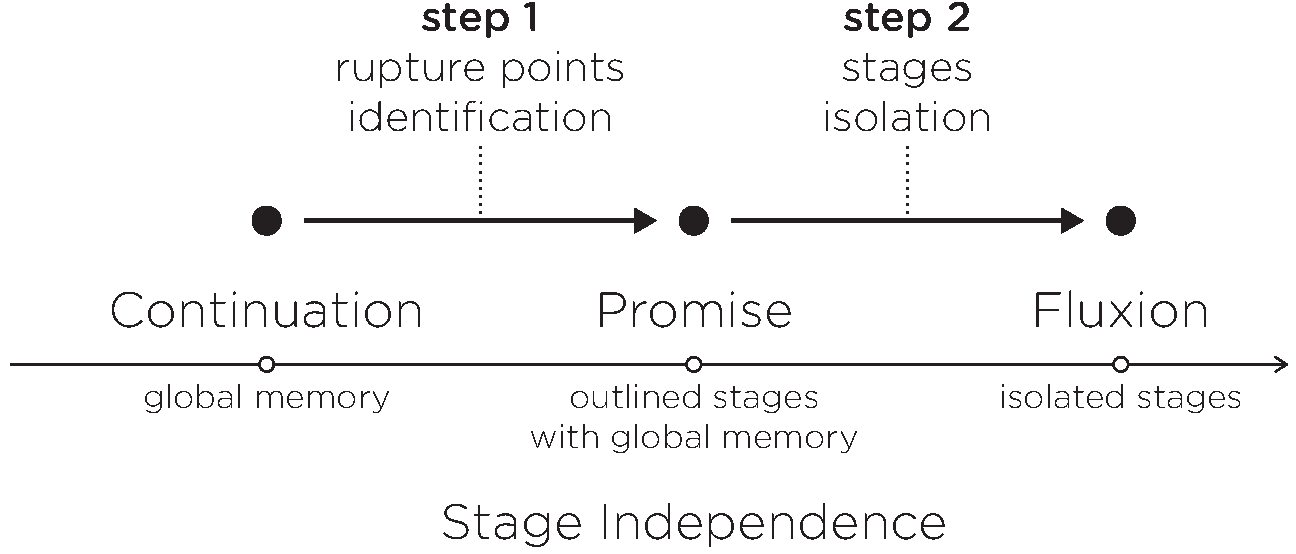
\includegraphics[width=0.7\textwidth]{../resources/roadmap.pdf}%
    \caption{Roadmap}%
    \label{fig:roadmap}%
  }%
\end{figure}

The first compiler focuses on the identification of simple chains of causality between continuations to transform these chains into Promises.
% the transformation from continuations to Promises.
% It focuses on the identification of the chains of causality in continuations.
However, promises are more expressive than the simple chaining of causal sequentiality.
% They force another control over the execution flow.
% According to the outcome of the operation, they call one function to continue the execution with the result, or another to handle errors.
% This conditional execution is indivisible from the Promise specification.
% Promises impose a convention on how to hand back the outcome of the deferred computation, while classic continuations leave this conditional execution to the developer.
Moreover, they impose a different convention than continuations on how to hand back the outcome and errors of the deferred computation.
This difference brings unnecessary complexity to the identification of chains.
To rule out this difference between continuations and Promises, before introducing the first compiler, section \ref{chapter5:due} introduces a simpler specification to Promise, called Due.

The second compiler detects all the chains of causality between continuations and encapsulate them in fluxions.
It isolates the fluxions when possible to allow the parallelism required for efficiency.
This second compilers is introduced in section \ref{chapter5:flx}.

\input{05-implementation/Due/main}
\input{05-implementation/Flx/main}
% \input{05-implementation/Evaluation}

% \subsection{Real test case} \label{chapter5:flx:evaluation}

The compiler is tested on a real application, gifsockets-server\ftnt{https://github.com/twolfson/gifsockets-server}.
This test proves the possibility for an application to be compiled into a network of independent parts.
It shows the current limitations of this isolation and the modifications needed on the application to circumvent them.

\begin{code}[js, caption={Simplified version of gifsockets-server},label={lst:gifsocket}]
var express = require('express'),
    app = express(),
    routes = require('gifsockets-middleware'), //@\label{lst:gifsocket:gif-mw}@
    getRawBody = require('raw-body');

function bodyParser(limit) { //@\label{lst:gifsocket:bodyParser}@
  return function saveBody(req, res, next) { //@\label{lst:gifsocket:saveBody}@
    getRawBody(req, { //@\label{lst:gifsocket:getRawBody}@
      expected: req.headers['content-length'],
      limit: limit
    }, function (err, buffer) { //@\label{lst:gifsocket:callback}@
      req.body = buffer;
      next(); //@\label{lst:gifsocket:next}@
    });
  };
}

app.post('/image/text', bodyParser(1 * 1024 * 1024), routes.writeTextToImages); //@\label{lst:gifsocket:app.post}@
app.listen(8000);
\end{code}

This application, simplified in listing \ref{lst:gifsocket}, is a real-time chat using gif-based communication channels.
It was selected from the evaluation set of the Due compiler because it is simple enough to illustrate this evaluation.
% \cite{Brodu2015}
%  from the \texttt{npm} registry because it depends on \texttt{express}, it is tested, working, and simple enough to illustrate this evaluation.
The server transforms the received text into a gif frame, and pushes it back to a never-ending gif to be displayed on the client.

On line \ref{lst:gifsocket:app.post}, the application registers two functions to process the requests received on the url \texttt{/image/text}.
The closure \texttt{saveBody}, line \ref{lst:gifsocket:saveBody}, returned by \texttt{bodyParser}, line \ref{lst:gifsocket:bodyParser}, and the method \texttt{routes.write\-Text\-To\-Images} from the external module \texttt{gifsockets-\-middleware}, line \ref{lst:gifsocket:gif-mw}.
The closure \texttt{saveBody} calls the asynchronous function \texttt{getRawBody} to get the request body.
Its callback handles the errors, and calls \texttt{next} to continue processing the request with the next function, \texttt{routes.write\-Text\-To\-Images}.

\subsubsection{Compilation} \label{chapter5:flx:evaluation:compilation}

% We compile this application with the compiler
The compilation result is in listing \ref{lst:flx-gifsocket}.
The function call \texttt{app.post}, line \ref{lst:gifsocket:app.post}, is a rupture point.
However, its callbacks, \texttt{bodyParser} and \texttt{routes.write\-Text\-To\-Images} are not declared \textit{in situ}.
They are evaluated as functions only at runtime.
As precised previously, the compiler discards these callbacks to avoid altering the semantic. % by moving or modifying their definition.
% For this reason, the compiler ignores this rupture point, to avoid interfering with the evaluation.

\begin{code}[flx, caption={Compilation result of gifsockets-server},label={lst:flx-gifsocket}]
flx main & express {req}
>> anonymous_1000 [req, next]
  var express = require('express'),
      app = express(),
      routes = require('gifsockets-middleware'), //@\label{lst:flx-gifsocket:gif-mw}@
      getRawBody = require('raw-body');

  function bodyParser(limit) { //@\label{lst:flx-gifsocket:bodyParser}@
    return function saveBody(req, res, next) { //@\label{lst:flx-gifsocket:saveBody}@
      getRawBody(req, { //@\label{lst:flx-gifsocket:getRawBody}@
        expected: req.headers['content-length'], //@\label{lst:flx-gifsocket:req.headers}@
        limit: limit
      }, >> anonymous_1000 [req, next]);
    };
  }

  app.post('/image/text', bodyParser(1 * 1024 * 1024), routes.writeTextToImages); //@\label{lst:flx-gifsocket:app.post}@
  app.listen(8000);

flx anonymous_1000
-> null
  function (err, buffer) { //@\label{lst:flx-gifsocket:callback}@
    req.body = buffer; //@\label{lst:flx-gifsocket:buffer}@
    next(); //@\label{lst:flx-gifsocket:next}@
  }
\end{code}

The compiler detects a rupture point : the function \texttt{get\-Raw\-Body} and its anonymous callback, line \ref{lst:gifsocket:callback}.
It encapsulates this callback in a fluxion named \texttt{anony\-mous\_\-1000}.
The callback is replaced with a stream placeholder to send the message stream to this downstream fluxion.
The variables \texttt{req} and \texttt{next} are appended to this message stream, to propagate their value from the \texttt{main} fluxion to the \texttt{anony\-mous\_\-1000} fluxion.

When \texttt{anony\-mous\_\-1000} is not isolated from the \texttt{main} fluxion, as if they belong to the same group, the compilation result works as expected.
The variables used in the fluxion, \texttt{req} and \texttt{next}, are still shared between the two fluxions.
In this situation fluxions are quite similar to Dues regarding memory shareing.
Our goal is to isolate the two fluxions, to be able to safely parallelize their executions.

\subsubsection{Isolation} \label{chapter5:flx:evaluation:isolation}

In listing \ref{lst:flx-gifsocket}, the fluxion \texttt{anony\-mous\_\-1000} modifies the object \texttt{req}, line \ref{lst:flx-gifsocket:buffer}, to store the text of the received request, and it calls \texttt{next} to continue the execution, line \ref{lst:flx-gifsocket:next}.
\texttt{req} is an alias to a memory location used in multiple palces in code.
Therefore, these operations produce side-effects that should propagate in the whole application, but the isolation prevents this propagation.
Isolating the fluxion \texttt{anony\-mous\_\-1000} produces runtime exceptions.
The next paragraph details how this situation is handled to allow the application to be parallelized.

\paragraph{Variable \texttt{req}}

The variable \texttt{req} is read in fluxion \texttt{main}, lines \ref{lst:flx-gifsocket:getRawBody} and \ref{lst:flx-gifsocket:req.headers}.
Then its property \texttt{body} is associated to \texttt{buffer} in fluxion \texttt{anony\-mous\_\-1000}, line \ref{lst:flx-gifsocket:buffer}.
The compiler is unable to identify the aliases of this variable. % further usages.
However, the side effect resulting from this association impacts a variable in the scope of the next callback, \texttt{routes.write\-Text\-To\-Images}.
In this test case, the application is modified manually to explicitly propagate this side-effect to the next callback through the function \texttt{next}.
The modifications of this function are explained further in the next paragraph.

\paragraph{Closure \texttt{next}}

The function \texttt{next} is a closure provided by the \texttt{express} \texttt{Router} to continue the execution with the next function to handle the client request.
Because it indirectly relies on the variable \texttt{req}, it is impossible to isolate its execution with the \texttt{anony\-mous\_\-1000} fluxion.
Instead, we modify \texttt{express}, so as to be compatible with the fluxional execution model.
We explain the modifications below.

\begin{code}[flx, caption={Simplified modification on the compiled result},label={lst:mflx-gifsocket}]
flx anonymous_1000
-> express_dispatcher
  function (err, buffer) { //@\label{lst:mflx-gifsocket:callback}@
    req.body = buffer; //@\label{lst:mflx-gifsocket:buffer}@
    next_placeholder(req, -> express_dispatcher); //@\label{lst:mflx-gifsocket:next-placeholder}@
  }

flx express_dispatcher & express {req} //@\label{lst:mflx-gifsocket:express-dispatcher}@
-> null
  function (modified_req) {
    merge(req, modified_req);
    next(); //@\label{lst:mflx-gifsocket:next}@
  }
\end{code}

In listing \ref{lst:gifsocket}, the function \texttt{next} is a continuation allowing the anonymous callback, line \ref{lst:gifsocket:callback}, to call the next function to handle the request.
To isolate the anonymous callback into \texttt{anonymous\_\-1000}, \texttt{next} is replaced by a rupture point.
This replacement is illustrated in listing \ref{lst:mflx-gifsocket}.
The \texttt{express} \texttt{Router} registers a fluxion named \texttt{express\_\-dispatcher}, line \ref{lst:mflx-gifsocket:express-dispatcher}, to continue the execution after the fluxion \texttt{anony\-mous\_\-1000}.
This fluxion is in the same group \texttt{express} as the \texttt{main} fluxion, hence it has access to the original variable \texttt{req}, and to the original function \texttt{next}.
The call to the original \texttt{next} function is replaced by a placeholder to push the stream to the fluxion \texttt{express\_\-dispatcher}, line \ref{lst:mflx-gifsocket:next-placeholder}.
The fluxion \texttt{express\_\-dispatcher} receives the stream from the upstream fluxion \texttt{anony\-mous\_\-1000}, merges back the modification in the variable \texttt{req} to propagate the side effects, and finally calls the original function \texttt{next} to continue the execution, line \ref{lst:mflx-gifsocket:next}.

After the modifications detailed above, the server works as expected.
The isolated fluxion correctly receives, and returns its serialized messages.
The client successfully receives a gif frame containing the text.



\subsection{Limitations}

The static analysis used for this compiler presents some limitations.
It is unable to analyze code with dynamic behaviors.
Higher-order programming leads to more productivity partly beacuse it rely on such dynamic behavior to extend expressivity.
Precisely, it allows more levels of indirections.

\subsubsection{Levels of Indirections}

The indirection is an abstraction between the value, and its manipulation.
In listing \ref{lst:indirection}, the variables \texttt{a} and \texttt{b} point both to the same memory object.
The function \texttt{fn} introduces a level of indirection between the real object \texttt{a} and its manipulation handle, \texttt{b};
% Actually, the variable \texttt{a} already introduces a level of indirection between the real object and the handle \texttt{a}.

\begin{code}[js,
  caption={One level of Indirection},
  label={lst:indirection}]
var a = {
      // an object;
    };

fn(b) {
  // modify b;
}

fn(a);
\end{code}

\subsubsection{Uncertainties}

The indirection is trivial to resolve in listing \ref{lst:indirection}.
It only needs to have access to the definition of \texttt{a} and of \texttt{fn}.
%A very simple static analysis could resolve it.
However, in listing \ref{lst:indirections}, the array \texttt{handlers} introduces a new level of indirection.
The static analysis now needs to have access to the definition of \texttt{i} and of the \texttt{handlers}.
If this definition is provided by an external input, it is not available statically, hence, it adds an uncertainty during the analysis. 

\begin{code}[js,
  caption={Two levels of indirection},
  label={lst:indirections}]
var a = {
      // an object;
    },
    handlers = [
      // definition of fn handlers;
    ],
    i = ?;

handlers[i](a);
handlers[i+1](a);
\end{code}

These examples are extremely simplified.
A real application contains enough indirections for the static analysis to be overwhelmed by uncertainties, and to be unable to resolve the variables.
If a variable is left unresolved, it is impossible to assure its scope and its aliases.
Therefore, the compiler is unable to isolate it into a fluxion, or to distribute its modification by messages.

Moreover, it leads the compiler to ignore the rupture points not defined \textit{in situ}, because their modifications could impact the semantic.
The reason for this precaution, is that the compiler is unable to assure where the function is used, and the scope of its variables.
Therefore, it is unable to assure that the modification will conserve the semantic.

\subsubsection{Dynamic Resolution}

In a web application, this variable \texttt{i} might be part of the user request, which is available only at runtime.
It eventually introduces an uncertainty.

This dynamic resolution of variables is precisely what increase expressiveness.
Trying to resolve them statically is equivalent to restrict expressiveness.
No static analysis can overstep these limitations.
Only a dynamic analysis could analysis the resolved indirections during run time to overstep these limitations correctly.




\renewcommand{\glyph}{\iconfont{\XeTeXglyph287}}
\chapter{Implementations} \label{chapter5}
\minitoc
\eject
The transformation allowed by the equivalence from an event-driven program into a distributed network of fluxions is implemented incrementally into two compilers, as presented in figure \ref{fig:roadmap}.
Each compilers is divided into two steps, the identification of the rupture points separating the stages of the pipeline, and the isolation of these stages.
% This chapter presents the technical implementations of these two steps in the transformation from the event-driven execution model to the pipeline architecture
% , the transformation described in the previous chapter was implemented incrementally in two compilers.

\begin{figure}[h!]%
  \textfig{%
    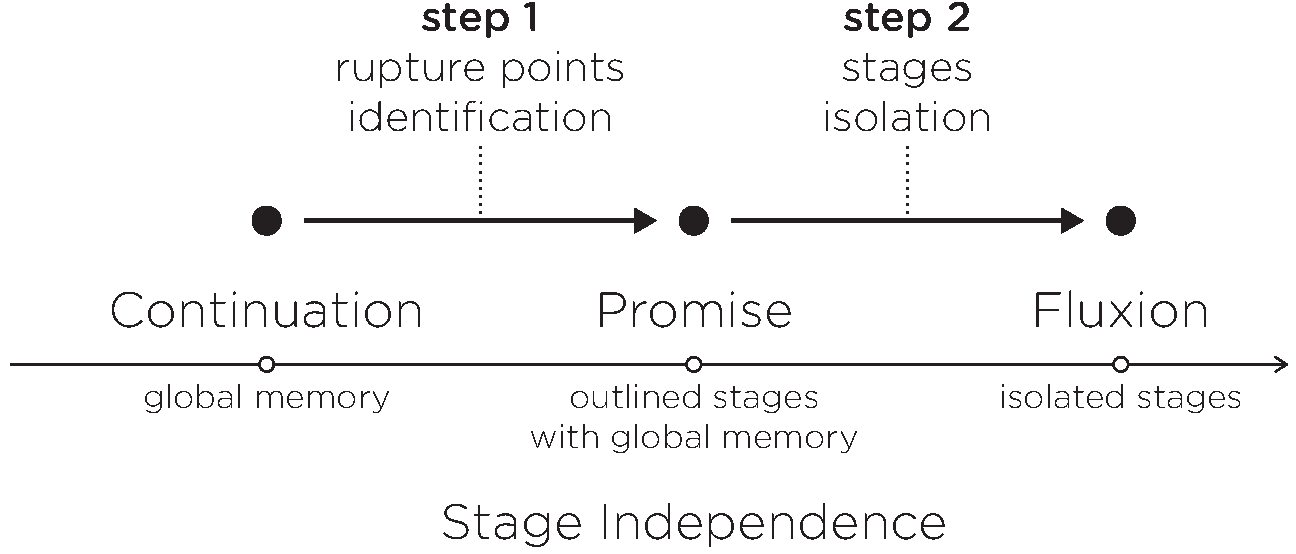
\includegraphics[width=0.7\textwidth]{../resources/roadmap.pdf}%
    \caption{Roadmap}%
    \label{fig:roadmap}%
  }%
\end{figure}

The first compiler focuses on the identification of simple chains of causality between continuations to transform these chains into Promises.
% the transformation from continuations to Promises.
% It focuses on the identification of the chains of causality in continuations.
However, promises are more expressive than the simple chaining of causal sequentiality.
% They force another control over the execution flow.
% According to the outcome of the operation, they call one function to continue the execution with the result, or another to handle errors.
% This conditional execution is indivisible from the Promise specification.
% Promises impose a convention on how to hand back the outcome of the deferred computation, while classic continuations leave this conditional execution to the developer.
Moreover, they impose a different convention than continuations on how to hand back the outcome and errors of the deferred computation.
This difference brings unnecessary complexity to the identification of chains.
To rule out this difference between continuations and Promises, before introducing the first compiler, section \ref{chapter5:due} introduces a simpler specification to Promise, called Due.

The second compiler detects all the chains of causality between continuations and encapsulate them in fluxions.
It isolates the fluxions when possible to allow the parallelism required for efficiency.
This second compilers is introduced in section \ref{chapter5:flx}.

\renewcommand{\glyph}{\iconfont{\XeTeXglyph287}}
\chapter{Implementations} \label{chapter5}
\minitoc
\eject
The transformation allowed by the equivalence from an event-driven program into a distributed network of fluxions is implemented incrementally into two compilers, as presented in figure \ref{fig:roadmap}.
Each compilers is divided into two steps, the identification of the rupture points separating the stages of the pipeline, and the isolation of these stages.
% This chapter presents the technical implementations of these two steps in the transformation from the event-driven execution model to the pipeline architecture
% , the transformation described in the previous chapter was implemented incrementally in two compilers.

\begin{figure}[h!]%
  \textfig{%
    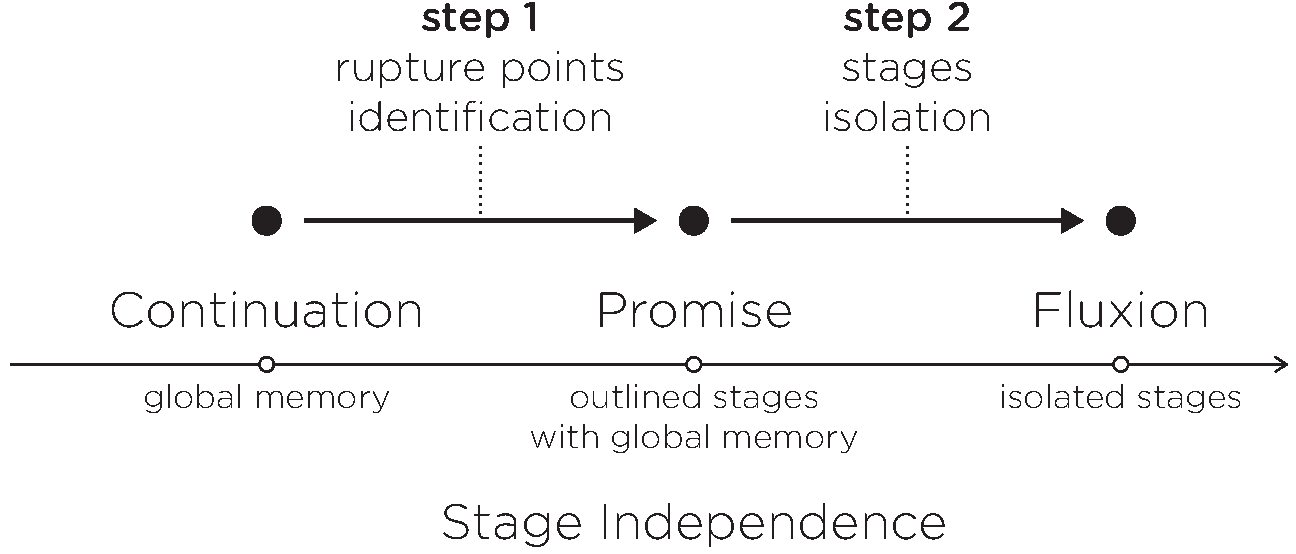
\includegraphics[width=0.7\textwidth]{../resources/roadmap.pdf}%
    \caption{Roadmap}%
    \label{fig:roadmap}%
  }%
\end{figure}

The first compiler focuses on the identification of simple chains of causality between continuations to transform these chains into Promises.
% the transformation from continuations to Promises.
% It focuses on the identification of the chains of causality in continuations.
However, promises are more expressive than the simple chaining of causal sequentiality.
% They force another control over the execution flow.
% According to the outcome of the operation, they call one function to continue the execution with the result, or another to handle errors.
% This conditional execution is indivisible from the Promise specification.
% Promises impose a convention on how to hand back the outcome of the deferred computation, while classic continuations leave this conditional execution to the developer.
Moreover, they impose a different convention than continuations on how to hand back the outcome and errors of the deferred computation.
This difference brings unnecessary complexity to the identification of chains.
To rule out this difference between continuations and Promises, before introducing the first compiler, section \ref{chapter5:due} introduces a simpler specification to Promise, called Due.

The second compiler detects all the chains of causality between continuations and encapsulate them in fluxions.
It isolates the fluxions when possible to allow the parallelism required for efficiency.
This second compilers is introduced in section \ref{chapter5:flx}.

\input{05-implementation/Due/main}
\input{05-implementation/Flx/main}
% \input{05-implementation/Evaluation}

\renewcommand{\glyph}{\iconfont{\XeTeXglyph287}}
\chapter{Implementations} \label{chapter5}
\minitoc
\eject
The transformation allowed by the equivalence from an event-driven program into a distributed network of fluxions is implemented incrementally into two compilers, as presented in figure \ref{fig:roadmap}.
Each compilers is divided into two steps, the identification of the rupture points separating the stages of the pipeline, and the isolation of these stages.
% This chapter presents the technical implementations of these two steps in the transformation from the event-driven execution model to the pipeline architecture
% , the transformation described in the previous chapter was implemented incrementally in two compilers.

\begin{figure}[h!]%
  \textfig{%
    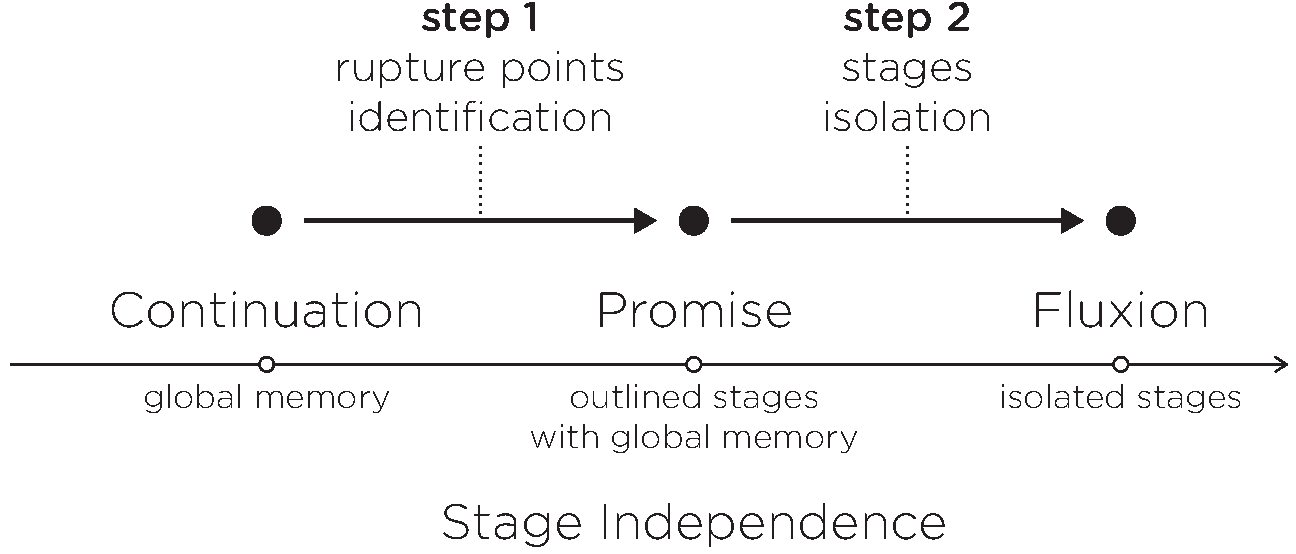
\includegraphics[width=0.7\textwidth]{../resources/roadmap.pdf}%
    \caption{Roadmap}%
    \label{fig:roadmap}%
  }%
\end{figure}

The first compiler focuses on the identification of simple chains of causality between continuations to transform these chains into Promises.
% the transformation from continuations to Promises.
% It focuses on the identification of the chains of causality in continuations.
However, promises are more expressive than the simple chaining of causal sequentiality.
% They force another control over the execution flow.
% According to the outcome of the operation, they call one function to continue the execution with the result, or another to handle errors.
% This conditional execution is indivisible from the Promise specification.
% Promises impose a convention on how to hand back the outcome of the deferred computation, while classic continuations leave this conditional execution to the developer.
Moreover, they impose a different convention than continuations on how to hand back the outcome and errors of the deferred computation.
This difference brings unnecessary complexity to the identification of chains.
To rule out this difference between continuations and Promises, before introducing the first compiler, section \ref{chapter5:due} introduces a simpler specification to Promise, called Due.

The second compiler detects all the chains of causality between continuations and encapsulate them in fluxions.
It isolates the fluxions when possible to allow the parallelism required for efficiency.
This second compilers is introduced in section \ref{chapter5:flx}.

\input{05-implementation/Due/main}
\input{05-implementation/Flx/main}
% \input{05-implementation/Evaluation}

% \subsection{Real test case} \label{chapter5:flx:evaluation}

The compiler is tested on a real application, gifsockets-server\ftnt{https://github.com/twolfson/gifsockets-server}.
This test proves the possibility for an application to be compiled into a network of independent parts.
It shows the current limitations of this isolation and the modifications needed on the application to circumvent them.

\begin{code}[js, caption={Simplified version of gifsockets-server},label={lst:gifsocket}]
var express = require('express'),
    app = express(),
    routes = require('gifsockets-middleware'), //@\label{lst:gifsocket:gif-mw}@
    getRawBody = require('raw-body');

function bodyParser(limit) { //@\label{lst:gifsocket:bodyParser}@
  return function saveBody(req, res, next) { //@\label{lst:gifsocket:saveBody}@
    getRawBody(req, { //@\label{lst:gifsocket:getRawBody}@
      expected: req.headers['content-length'],
      limit: limit
    }, function (err, buffer) { //@\label{lst:gifsocket:callback}@
      req.body = buffer;
      next(); //@\label{lst:gifsocket:next}@
    });
  };
}

app.post('/image/text', bodyParser(1 * 1024 * 1024), routes.writeTextToImages); //@\label{lst:gifsocket:app.post}@
app.listen(8000);
\end{code}

This application, simplified in listing \ref{lst:gifsocket}, is a real-time chat using gif-based communication channels.
It was selected from the evaluation set of the Due compiler because it is simple enough to illustrate this evaluation.
% \cite{Brodu2015}
%  from the \texttt{npm} registry because it depends on \texttt{express}, it is tested, working, and simple enough to illustrate this evaluation.
The server transforms the received text into a gif frame, and pushes it back to a never-ending gif to be displayed on the client.

On line \ref{lst:gifsocket:app.post}, the application registers two functions to process the requests received on the url \texttt{/image/text}.
The closure \texttt{saveBody}, line \ref{lst:gifsocket:saveBody}, returned by \texttt{bodyParser}, line \ref{lst:gifsocket:bodyParser}, and the method \texttt{routes.write\-Text\-To\-Images} from the external module \texttt{gifsockets-\-middleware}, line \ref{lst:gifsocket:gif-mw}.
The closure \texttt{saveBody} calls the asynchronous function \texttt{getRawBody} to get the request body.
Its callback handles the errors, and calls \texttt{next} to continue processing the request with the next function, \texttt{routes.write\-Text\-To\-Images}.

\subsubsection{Compilation} \label{chapter5:flx:evaluation:compilation}

% We compile this application with the compiler
The compilation result is in listing \ref{lst:flx-gifsocket}.
The function call \texttt{app.post}, line \ref{lst:gifsocket:app.post}, is a rupture point.
However, its callbacks, \texttt{bodyParser} and \texttt{routes.write\-Text\-To\-Images} are not declared \textit{in situ}.
They are evaluated as functions only at runtime.
As precised previously, the compiler discards these callbacks to avoid altering the semantic. % by moving or modifying their definition.
% For this reason, the compiler ignores this rupture point, to avoid interfering with the evaluation.

\begin{code}[flx, caption={Compilation result of gifsockets-server},label={lst:flx-gifsocket}]
flx main & express {req}
>> anonymous_1000 [req, next]
  var express = require('express'),
      app = express(),
      routes = require('gifsockets-middleware'), //@\label{lst:flx-gifsocket:gif-mw}@
      getRawBody = require('raw-body');

  function bodyParser(limit) { //@\label{lst:flx-gifsocket:bodyParser}@
    return function saveBody(req, res, next) { //@\label{lst:flx-gifsocket:saveBody}@
      getRawBody(req, { //@\label{lst:flx-gifsocket:getRawBody}@
        expected: req.headers['content-length'], //@\label{lst:flx-gifsocket:req.headers}@
        limit: limit
      }, >> anonymous_1000 [req, next]);
    };
  }

  app.post('/image/text', bodyParser(1 * 1024 * 1024), routes.writeTextToImages); //@\label{lst:flx-gifsocket:app.post}@
  app.listen(8000);

flx anonymous_1000
-> null
  function (err, buffer) { //@\label{lst:flx-gifsocket:callback}@
    req.body = buffer; //@\label{lst:flx-gifsocket:buffer}@
    next(); //@\label{lst:flx-gifsocket:next}@
  }
\end{code}

The compiler detects a rupture point : the function \texttt{get\-Raw\-Body} and its anonymous callback, line \ref{lst:gifsocket:callback}.
It encapsulates this callback in a fluxion named \texttt{anony\-mous\_\-1000}.
The callback is replaced with a stream placeholder to send the message stream to this downstream fluxion.
The variables \texttt{req} and \texttt{next} are appended to this message stream, to propagate their value from the \texttt{main} fluxion to the \texttt{anony\-mous\_\-1000} fluxion.

When \texttt{anony\-mous\_\-1000} is not isolated from the \texttt{main} fluxion, as if they belong to the same group, the compilation result works as expected.
The variables used in the fluxion, \texttt{req} and \texttt{next}, are still shared between the two fluxions.
In this situation fluxions are quite similar to Dues regarding memory shareing.
Our goal is to isolate the two fluxions, to be able to safely parallelize their executions.

\subsubsection{Isolation} \label{chapter5:flx:evaluation:isolation}

In listing \ref{lst:flx-gifsocket}, the fluxion \texttt{anony\-mous\_\-1000} modifies the object \texttt{req}, line \ref{lst:flx-gifsocket:buffer}, to store the text of the received request, and it calls \texttt{next} to continue the execution, line \ref{lst:flx-gifsocket:next}.
\texttt{req} is an alias to a memory location used in multiple palces in code.
Therefore, these operations produce side-effects that should propagate in the whole application, but the isolation prevents this propagation.
Isolating the fluxion \texttt{anony\-mous\_\-1000} produces runtime exceptions.
The next paragraph details how this situation is handled to allow the application to be parallelized.

\paragraph{Variable \texttt{req}}

The variable \texttt{req} is read in fluxion \texttt{main}, lines \ref{lst:flx-gifsocket:getRawBody} and \ref{lst:flx-gifsocket:req.headers}.
Then its property \texttt{body} is associated to \texttt{buffer} in fluxion \texttt{anony\-mous\_\-1000}, line \ref{lst:flx-gifsocket:buffer}.
The compiler is unable to identify the aliases of this variable. % further usages.
However, the side effect resulting from this association impacts a variable in the scope of the next callback, \texttt{routes.write\-Text\-To\-Images}.
In this test case, the application is modified manually to explicitly propagate this side-effect to the next callback through the function \texttt{next}.
The modifications of this function are explained further in the next paragraph.

\paragraph{Closure \texttt{next}}

The function \texttt{next} is a closure provided by the \texttt{express} \texttt{Router} to continue the execution with the next function to handle the client request.
Because it indirectly relies on the variable \texttt{req}, it is impossible to isolate its execution with the \texttt{anony\-mous\_\-1000} fluxion.
Instead, we modify \texttt{express}, so as to be compatible with the fluxional execution model.
We explain the modifications below.

\begin{code}[flx, caption={Simplified modification on the compiled result},label={lst:mflx-gifsocket}]
flx anonymous_1000
-> express_dispatcher
  function (err, buffer) { //@\label{lst:mflx-gifsocket:callback}@
    req.body = buffer; //@\label{lst:mflx-gifsocket:buffer}@
    next_placeholder(req, -> express_dispatcher); //@\label{lst:mflx-gifsocket:next-placeholder}@
  }

flx express_dispatcher & express {req} //@\label{lst:mflx-gifsocket:express-dispatcher}@
-> null
  function (modified_req) {
    merge(req, modified_req);
    next(); //@\label{lst:mflx-gifsocket:next}@
  }
\end{code}

In listing \ref{lst:gifsocket}, the function \texttt{next} is a continuation allowing the anonymous callback, line \ref{lst:gifsocket:callback}, to call the next function to handle the request.
To isolate the anonymous callback into \texttt{anonymous\_\-1000}, \texttt{next} is replaced by a rupture point.
This replacement is illustrated in listing \ref{lst:mflx-gifsocket}.
The \texttt{express} \texttt{Router} registers a fluxion named \texttt{express\_\-dispatcher}, line \ref{lst:mflx-gifsocket:express-dispatcher}, to continue the execution after the fluxion \texttt{anony\-mous\_\-1000}.
This fluxion is in the same group \texttt{express} as the \texttt{main} fluxion, hence it has access to the original variable \texttt{req}, and to the original function \texttt{next}.
The call to the original \texttt{next} function is replaced by a placeholder to push the stream to the fluxion \texttt{express\_\-dispatcher}, line \ref{lst:mflx-gifsocket:next-placeholder}.
The fluxion \texttt{express\_\-dispatcher} receives the stream from the upstream fluxion \texttt{anony\-mous\_\-1000}, merges back the modification in the variable \texttt{req} to propagate the side effects, and finally calls the original function \texttt{next} to continue the execution, line \ref{lst:mflx-gifsocket:next}.

After the modifications detailed above, the server works as expected.
The isolated fluxion correctly receives, and returns its serialized messages.
The client successfully receives a gif frame containing the text.



\subsection{Limitations}

The static analysis used for this compiler presents some limitations.
It is unable to analyze code with dynamic behaviors.
Higher-order programming leads to more productivity partly beacuse it rely on such dynamic behavior to extend expressivity.
Precisely, it allows more levels of indirections.

\subsubsection{Levels of Indirections}

The indirection is an abstraction between the value, and its manipulation.
In listing \ref{lst:indirection}, the variables \texttt{a} and \texttt{b} point both to the same memory object.
The function \texttt{fn} introduces a level of indirection between the real object \texttt{a} and its manipulation handle, \texttt{b};
% Actually, the variable \texttt{a} already introduces a level of indirection between the real object and the handle \texttt{a}.

\begin{code}[js,
  caption={One level of Indirection},
  label={lst:indirection}]
var a = {
      // an object;
    };

fn(b) {
  // modify b;
}

fn(a);
\end{code}

\subsubsection{Uncertainties}

The indirection is trivial to resolve in listing \ref{lst:indirection}.
It only needs to have access to the definition of \texttt{a} and of \texttt{fn}.
%A very simple static analysis could resolve it.
However, in listing \ref{lst:indirections}, the array \texttt{handlers} introduces a new level of indirection.
The static analysis now needs to have access to the definition of \texttt{i} and of the \texttt{handlers}.
If this definition is provided by an external input, it is not available statically, hence, it adds an uncertainty during the analysis. 

\begin{code}[js,
  caption={Two levels of indirection},
  label={lst:indirections}]
var a = {
      // an object;
    },
    handlers = [
      // definition of fn handlers;
    ],
    i = ?;

handlers[i](a);
handlers[i+1](a);
\end{code}

These examples are extremely simplified.
A real application contains enough indirections for the static analysis to be overwhelmed by uncertainties, and to be unable to resolve the variables.
If a variable is left unresolved, it is impossible to assure its scope and its aliases.
Therefore, the compiler is unable to isolate it into a fluxion, or to distribute its modification by messages.

Moreover, it leads the compiler to ignore the rupture points not defined \textit{in situ}, because their modifications could impact the semantic.
The reason for this precaution, is that the compiler is unable to assure where the function is used, and the scope of its variables.
Therefore, it is unable to assure that the modification will conserve the semantic.

\subsubsection{Dynamic Resolution}

In a web application, this variable \texttt{i} might be part of the user request, which is available only at runtime.
It eventually introduces an uncertainty.

This dynamic resolution of variables is precisely what increase expressiveness.
Trying to resolve them statically is equivalent to restrict expressiveness.
No static analysis can overstep these limitations.
Only a dynamic analysis could analysis the resolved indirections during run time to overstep these limitations correctly.




% \subsection{Real test case} \label{chapter5:flx:evaluation}

The compiler is tested on a real application, gifsockets-server\ftnt{https://github.com/twolfson/gifsockets-server}.
This test proves the possibility for an application to be compiled into a network of independent parts.
It shows the current limitations of this isolation and the modifications needed on the application to circumvent them.

\begin{code}[js, caption={Simplified version of gifsockets-server},label={lst:gifsocket}]
var express = require('express'),
    app = express(),
    routes = require('gifsockets-middleware'), //@\label{lst:gifsocket:gif-mw}@
    getRawBody = require('raw-body');

function bodyParser(limit) { //@\label{lst:gifsocket:bodyParser}@
  return function saveBody(req, res, next) { //@\label{lst:gifsocket:saveBody}@
    getRawBody(req, { //@\label{lst:gifsocket:getRawBody}@
      expected: req.headers['content-length'],
      limit: limit
    }, function (err, buffer) { //@\label{lst:gifsocket:callback}@
      req.body = buffer;
      next(); //@\label{lst:gifsocket:next}@
    });
  };
}

app.post('/image/text', bodyParser(1 * 1024 * 1024), routes.writeTextToImages); //@\label{lst:gifsocket:app.post}@
app.listen(8000);
\end{code}

This application, simplified in listing \ref{lst:gifsocket}, is a real-time chat using gif-based communication channels.
It was selected from the evaluation set of the Due compiler because it is simple enough to illustrate this evaluation.
% \cite{Brodu2015}
%  from the \texttt{npm} registry because it depends on \texttt{express}, it is tested, working, and simple enough to illustrate this evaluation.
The server transforms the received text into a gif frame, and pushes it back to a never-ending gif to be displayed on the client.

On line \ref{lst:gifsocket:app.post}, the application registers two functions to process the requests received on the url \texttt{/image/text}.
The closure \texttt{saveBody}, line \ref{lst:gifsocket:saveBody}, returned by \texttt{bodyParser}, line \ref{lst:gifsocket:bodyParser}, and the method \texttt{routes.write\-Text\-To\-Images} from the external module \texttt{gifsockets-\-middleware}, line \ref{lst:gifsocket:gif-mw}.
The closure \texttt{saveBody} calls the asynchronous function \texttt{getRawBody} to get the request body.
Its callback handles the errors, and calls \texttt{next} to continue processing the request with the next function, \texttt{routes.write\-Text\-To\-Images}.

\subsubsection{Compilation} \label{chapter5:flx:evaluation:compilation}

% We compile this application with the compiler
The compilation result is in listing \ref{lst:flx-gifsocket}.
The function call \texttt{app.post}, line \ref{lst:gifsocket:app.post}, is a rupture point.
However, its callbacks, \texttt{bodyParser} and \texttt{routes.write\-Text\-To\-Images} are not declared \textit{in situ}.
They are evaluated as functions only at runtime.
As precised previously, the compiler discards these callbacks to avoid altering the semantic. % by moving or modifying their definition.
% For this reason, the compiler ignores this rupture point, to avoid interfering with the evaluation.

\begin{code}[flx, caption={Compilation result of gifsockets-server},label={lst:flx-gifsocket}]
flx main & express {req}
>> anonymous_1000 [req, next]
  var express = require('express'),
      app = express(),
      routes = require('gifsockets-middleware'), //@\label{lst:flx-gifsocket:gif-mw}@
      getRawBody = require('raw-body');

  function bodyParser(limit) { //@\label{lst:flx-gifsocket:bodyParser}@
    return function saveBody(req, res, next) { //@\label{lst:flx-gifsocket:saveBody}@
      getRawBody(req, { //@\label{lst:flx-gifsocket:getRawBody}@
        expected: req.headers['content-length'], //@\label{lst:flx-gifsocket:req.headers}@
        limit: limit
      }, >> anonymous_1000 [req, next]);
    };
  }

  app.post('/image/text', bodyParser(1 * 1024 * 1024), routes.writeTextToImages); //@\label{lst:flx-gifsocket:app.post}@
  app.listen(8000);

flx anonymous_1000
-> null
  function (err, buffer) { //@\label{lst:flx-gifsocket:callback}@
    req.body = buffer; //@\label{lst:flx-gifsocket:buffer}@
    next(); //@\label{lst:flx-gifsocket:next}@
  }
\end{code}

The compiler detects a rupture point : the function \texttt{get\-Raw\-Body} and its anonymous callback, line \ref{lst:gifsocket:callback}.
It encapsulates this callback in a fluxion named \texttt{anony\-mous\_\-1000}.
The callback is replaced with a stream placeholder to send the message stream to this downstream fluxion.
The variables \texttt{req} and \texttt{next} are appended to this message stream, to propagate their value from the \texttt{main} fluxion to the \texttt{anony\-mous\_\-1000} fluxion.

When \texttt{anony\-mous\_\-1000} is not isolated from the \texttt{main} fluxion, as if they belong to the same group, the compilation result works as expected.
The variables used in the fluxion, \texttt{req} and \texttt{next}, are still shared between the two fluxions.
In this situation fluxions are quite similar to Dues regarding memory shareing.
Our goal is to isolate the two fluxions, to be able to safely parallelize their executions.

\subsubsection{Isolation} \label{chapter5:flx:evaluation:isolation}

In listing \ref{lst:flx-gifsocket}, the fluxion \texttt{anony\-mous\_\-1000} modifies the object \texttt{req}, line \ref{lst:flx-gifsocket:buffer}, to store the text of the received request, and it calls \texttt{next} to continue the execution, line \ref{lst:flx-gifsocket:next}.
\texttt{req} is an alias to a memory location used in multiple palces in code.
Therefore, these operations produce side-effects that should propagate in the whole application, but the isolation prevents this propagation.
Isolating the fluxion \texttt{anony\-mous\_\-1000} produces runtime exceptions.
The next paragraph details how this situation is handled to allow the application to be parallelized.

\paragraph{Variable \texttt{req}}

The variable \texttt{req} is read in fluxion \texttt{main}, lines \ref{lst:flx-gifsocket:getRawBody} and \ref{lst:flx-gifsocket:req.headers}.
Then its property \texttt{body} is associated to \texttt{buffer} in fluxion \texttt{anony\-mous\_\-1000}, line \ref{lst:flx-gifsocket:buffer}.
The compiler is unable to identify the aliases of this variable. % further usages.
However, the side effect resulting from this association impacts a variable in the scope of the next callback, \texttt{routes.write\-Text\-To\-Images}.
In this test case, the application is modified manually to explicitly propagate this side-effect to the next callback through the function \texttt{next}.
The modifications of this function are explained further in the next paragraph.

\paragraph{Closure \texttt{next}}

The function \texttt{next} is a closure provided by the \texttt{express} \texttt{Router} to continue the execution with the next function to handle the client request.
Because it indirectly relies on the variable \texttt{req}, it is impossible to isolate its execution with the \texttt{anony\-mous\_\-1000} fluxion.
Instead, we modify \texttt{express}, so as to be compatible with the fluxional execution model.
We explain the modifications below.

\begin{code}[flx, caption={Simplified modification on the compiled result},label={lst:mflx-gifsocket}]
flx anonymous_1000
-> express_dispatcher
  function (err, buffer) { //@\label{lst:mflx-gifsocket:callback}@
    req.body = buffer; //@\label{lst:mflx-gifsocket:buffer}@
    next_placeholder(req, -> express_dispatcher); //@\label{lst:mflx-gifsocket:next-placeholder}@
  }

flx express_dispatcher & express {req} //@\label{lst:mflx-gifsocket:express-dispatcher}@
-> null
  function (modified_req) {
    merge(req, modified_req);
    next(); //@\label{lst:mflx-gifsocket:next}@
  }
\end{code}

In listing \ref{lst:gifsocket}, the function \texttt{next} is a continuation allowing the anonymous callback, line \ref{lst:gifsocket:callback}, to call the next function to handle the request.
To isolate the anonymous callback into \texttt{anonymous\_\-1000}, \texttt{next} is replaced by a rupture point.
This replacement is illustrated in listing \ref{lst:mflx-gifsocket}.
The \texttt{express} \texttt{Router} registers a fluxion named \texttt{express\_\-dispatcher}, line \ref{lst:mflx-gifsocket:express-dispatcher}, to continue the execution after the fluxion \texttt{anony\-mous\_\-1000}.
This fluxion is in the same group \texttt{express} as the \texttt{main} fluxion, hence it has access to the original variable \texttt{req}, and to the original function \texttt{next}.
The call to the original \texttt{next} function is replaced by a placeholder to push the stream to the fluxion \texttt{express\_\-dispatcher}, line \ref{lst:mflx-gifsocket:next-placeholder}.
The fluxion \texttt{express\_\-dispatcher} receives the stream from the upstream fluxion \texttt{anony\-mous\_\-1000}, merges back the modification in the variable \texttt{req} to propagate the side effects, and finally calls the original function \texttt{next} to continue the execution, line \ref{lst:mflx-gifsocket:next}.

After the modifications detailed above, the server works as expected.
The isolated fluxion correctly receives, and returns its serialized messages.
The client successfully receives a gif frame containing the text.



\subsection{Limitations}

The static analysis used for this compiler presents some limitations.
It is unable to analyze code with dynamic behaviors.
Higher-order programming leads to more productivity partly beacuse it rely on such dynamic behavior to extend expressivity.
Precisely, it allows more levels of indirections.

\subsubsection{Levels of Indirections}

The indirection is an abstraction between the value, and its manipulation.
In listing \ref{lst:indirection}, the variables \texttt{a} and \texttt{b} point both to the same memory object.
The function \texttt{fn} introduces a level of indirection between the real object \texttt{a} and its manipulation handle, \texttt{b};
% Actually, the variable \texttt{a} already introduces a level of indirection between the real object and the handle \texttt{a}.

\begin{code}[js,
  caption={One level of Indirection},
  label={lst:indirection}]
var a = {
      // an object;
    };

fn(b) {
  // modify b;
}

fn(a);
\end{code}

\subsubsection{Uncertainties}

The indirection is trivial to resolve in listing \ref{lst:indirection}.
It only needs to have access to the definition of \texttt{a} and of \texttt{fn}.
%A very simple static analysis could resolve it.
However, in listing \ref{lst:indirections}, the array \texttt{handlers} introduces a new level of indirection.
The static analysis now needs to have access to the definition of \texttt{i} and of the \texttt{handlers}.
If this definition is provided by an external input, it is not available statically, hence, it adds an uncertainty during the analysis. 

\begin{code}[js,
  caption={Two levels of indirection},
  label={lst:indirections}]
var a = {
      // an object;
    },
    handlers = [
      // definition of fn handlers;
    ],
    i = ?;

handlers[i](a);
handlers[i+1](a);
\end{code}

These examples are extremely simplified.
A real application contains enough indirections for the static analysis to be overwhelmed by uncertainties, and to be unable to resolve the variables.
If a variable is left unresolved, it is impossible to assure its scope and its aliases.
Therefore, the compiler is unable to isolate it into a fluxion, or to distribute its modification by messages.

Moreover, it leads the compiler to ignore the rupture points not defined \textit{in situ}, because their modifications could impact the semantic.
The reason for this precaution, is that the compiler is unable to assure where the function is used, and the scope of its variables.
Therefore, it is unable to assure that the modification will conserve the semantic.

\subsubsection{Dynamic Resolution}

In a web application, this variable \texttt{i} might be part of the user request, which is available only at runtime.
It eventually introduces an uncertainty.

This dynamic resolution of variables is precisely what increase expressiveness.
Trying to resolve them statically is equivalent to restrict expressiveness.
No static analysis can overstep these limitations.
Only a dynamic analysis could analysis the resolved indirections during run time to overstep these limitations correctly.




\renewcommand{\glyph}{\iconfont{\XeTeXglyph287}}
\chapter{Implementations} \label{chapter5}
\minitoc
\eject
The transformation allowed by the equivalence from an event-driven program into a distributed network of fluxions is implemented incrementally into two compilers, as presented in figure \ref{fig:roadmap}.
Each compilers is divided into two steps, the identification of the rupture points separating the stages of the pipeline, and the isolation of these stages.
% This chapter presents the technical implementations of these two steps in the transformation from the event-driven execution model to the pipeline architecture
% , the transformation described in the previous chapter was implemented incrementally in two compilers.

\begin{figure}[h!]%
  \textfig{%
    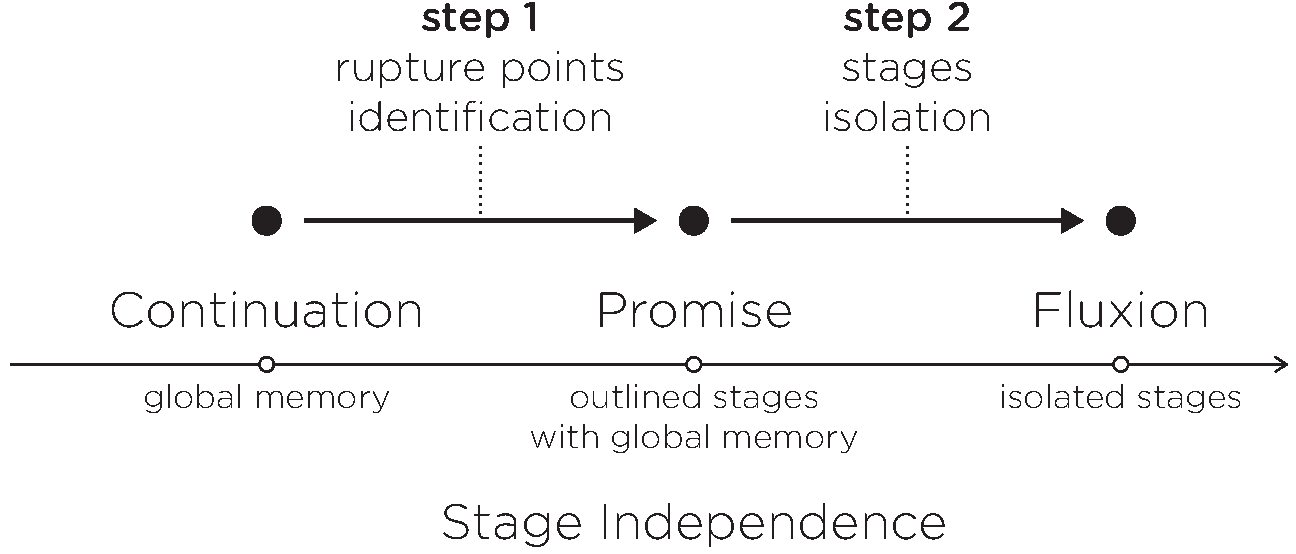
\includegraphics[width=0.7\textwidth]{../resources/roadmap.pdf}%
    \caption{Roadmap}%
    \label{fig:roadmap}%
  }%
\end{figure}

The first compiler focuses on the identification of simple chains of causality between continuations to transform these chains into Promises.
% the transformation from continuations to Promises.
% It focuses on the identification of the chains of causality in continuations.
However, promises are more expressive than the simple chaining of causal sequentiality.
% They force another control over the execution flow.
% According to the outcome of the operation, they call one function to continue the execution with the result, or another to handle errors.
% This conditional execution is indivisible from the Promise specification.
% Promises impose a convention on how to hand back the outcome of the deferred computation, while classic continuations leave this conditional execution to the developer.
Moreover, they impose a different convention than continuations on how to hand back the outcome and errors of the deferred computation.
This difference brings unnecessary complexity to the identification of chains.
To rule out this difference between continuations and Promises, before introducing the first compiler, section \ref{chapter5:due} introduces a simpler specification to Promise, called Due.

The second compiler detects all the chains of causality between continuations and encapsulate them in fluxions.
It isolates the fluxions when possible to allow the parallelism required for efficiency.
This second compilers is introduced in section \ref{chapter5:flx}.

\renewcommand{\glyph}{\iconfont{\XeTeXglyph287}}
\chapter{Implementations} \label{chapter5}
\minitoc
\eject
The transformation allowed by the equivalence from an event-driven program into a distributed network of fluxions is implemented incrementally into two compilers, as presented in figure \ref{fig:roadmap}.
Each compilers is divided into two steps, the identification of the rupture points separating the stages of the pipeline, and the isolation of these stages.
% This chapter presents the technical implementations of these two steps in the transformation from the event-driven execution model to the pipeline architecture
% , the transformation described in the previous chapter was implemented incrementally in two compilers.

\begin{figure}[h!]%
  \textfig{%
    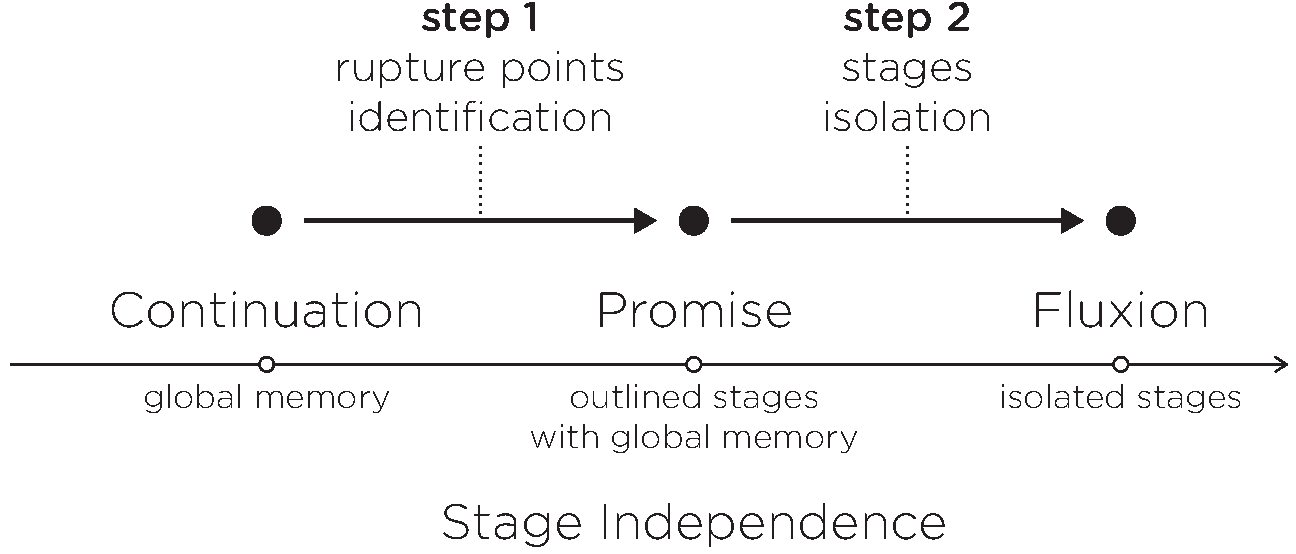
\includegraphics[width=0.7\textwidth]{../resources/roadmap.pdf}%
    \caption{Roadmap}%
    \label{fig:roadmap}%
  }%
\end{figure}

The first compiler focuses on the identification of simple chains of causality between continuations to transform these chains into Promises.
% the transformation from continuations to Promises.
% It focuses on the identification of the chains of causality in continuations.
However, promises are more expressive than the simple chaining of causal sequentiality.
% They force another control over the execution flow.
% According to the outcome of the operation, they call one function to continue the execution with the result, or another to handle errors.
% This conditional execution is indivisible from the Promise specification.
% Promises impose a convention on how to hand back the outcome of the deferred computation, while classic continuations leave this conditional execution to the developer.
Moreover, they impose a different convention than continuations on how to hand back the outcome and errors of the deferred computation.
This difference brings unnecessary complexity to the identification of chains.
To rule out this difference between continuations and Promises, before introducing the first compiler, section \ref{chapter5:due} introduces a simpler specification to Promise, called Due.

The second compiler detects all the chains of causality between continuations and encapsulate them in fluxions.
It isolates the fluxions when possible to allow the parallelism required for efficiency.
This second compilers is introduced in section \ref{chapter5:flx}.

\renewcommand{\glyph}{\iconfont{\XeTeXglyph287}}
\chapter{Implementations} \label{chapter5}
\minitoc
\eject
The transformation allowed by the equivalence from an event-driven program into a distributed network of fluxions is implemented incrementally into two compilers, as presented in figure \ref{fig:roadmap}.
Each compilers is divided into two steps, the identification of the rupture points separating the stages of the pipeline, and the isolation of these stages.
% This chapter presents the technical implementations of these two steps in the transformation from the event-driven execution model to the pipeline architecture
% , the transformation described in the previous chapter was implemented incrementally in two compilers.

\begin{figure}[h!]%
  \textfig{%
    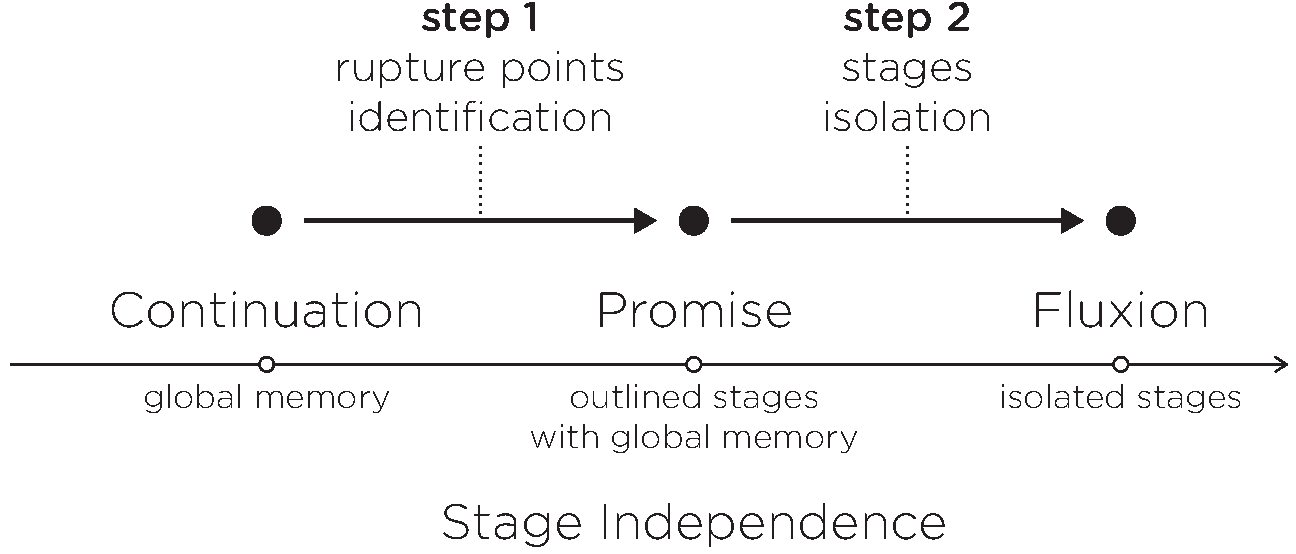
\includegraphics[width=0.7\textwidth]{../resources/roadmap.pdf}%
    \caption{Roadmap}%
    \label{fig:roadmap}%
  }%
\end{figure}

The first compiler focuses on the identification of simple chains of causality between continuations to transform these chains into Promises.
% the transformation from continuations to Promises.
% It focuses on the identification of the chains of causality in continuations.
However, promises are more expressive than the simple chaining of causal sequentiality.
% They force another control over the execution flow.
% According to the outcome of the operation, they call one function to continue the execution with the result, or another to handle errors.
% This conditional execution is indivisible from the Promise specification.
% Promises impose a convention on how to hand back the outcome of the deferred computation, while classic continuations leave this conditional execution to the developer.
Moreover, they impose a different convention than continuations on how to hand back the outcome and errors of the deferred computation.
This difference brings unnecessary complexity to the identification of chains.
To rule out this difference between continuations and Promises, before introducing the first compiler, section \ref{chapter5:due} introduces a simpler specification to Promise, called Due.

The second compiler detects all the chains of causality between continuations and encapsulate them in fluxions.
It isolates the fluxions when possible to allow the parallelism required for efficiency.
This second compilers is introduced in section \ref{chapter5:flx}.

\input{05-implementation/Due/main}
\input{05-implementation/Flx/main}
% \input{05-implementation/Evaluation}

\renewcommand{\glyph}{\iconfont{\XeTeXglyph287}}
\chapter{Implementations} \label{chapter5}
\minitoc
\eject
The transformation allowed by the equivalence from an event-driven program into a distributed network of fluxions is implemented incrementally into two compilers, as presented in figure \ref{fig:roadmap}.
Each compilers is divided into two steps, the identification of the rupture points separating the stages of the pipeline, and the isolation of these stages.
% This chapter presents the technical implementations of these two steps in the transformation from the event-driven execution model to the pipeline architecture
% , the transformation described in the previous chapter was implemented incrementally in two compilers.

\begin{figure}[h!]%
  \textfig{%
    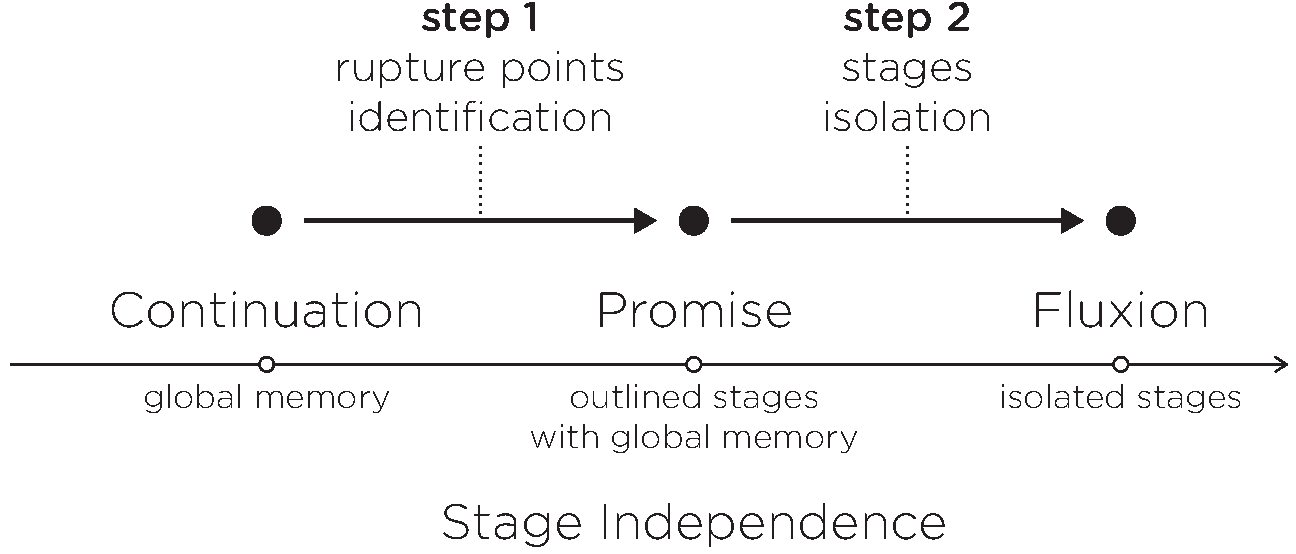
\includegraphics[width=0.7\textwidth]{../resources/roadmap.pdf}%
    \caption{Roadmap}%
    \label{fig:roadmap}%
  }%
\end{figure}

The first compiler focuses on the identification of simple chains of causality between continuations to transform these chains into Promises.
% the transformation from continuations to Promises.
% It focuses on the identification of the chains of causality in continuations.
However, promises are more expressive than the simple chaining of causal sequentiality.
% They force another control over the execution flow.
% According to the outcome of the operation, they call one function to continue the execution with the result, or another to handle errors.
% This conditional execution is indivisible from the Promise specification.
% Promises impose a convention on how to hand back the outcome of the deferred computation, while classic continuations leave this conditional execution to the developer.
Moreover, they impose a different convention than continuations on how to hand back the outcome and errors of the deferred computation.
This difference brings unnecessary complexity to the identification of chains.
To rule out this difference between continuations and Promises, before introducing the first compiler, section \ref{chapter5:due} introduces a simpler specification to Promise, called Due.

The second compiler detects all the chains of causality between continuations and encapsulate them in fluxions.
It isolates the fluxions when possible to allow the parallelism required for efficiency.
This second compilers is introduced in section \ref{chapter5:flx}.

\input{05-implementation/Due/main}
\input{05-implementation/Flx/main}
% \input{05-implementation/Evaluation}

% \subsection{Real test case} \label{chapter5:flx:evaluation}

The compiler is tested on a real application, gifsockets-server\ftnt{https://github.com/twolfson/gifsockets-server}.
This test proves the possibility for an application to be compiled into a network of independent parts.
It shows the current limitations of this isolation and the modifications needed on the application to circumvent them.

\begin{code}[js, caption={Simplified version of gifsockets-server},label={lst:gifsocket}]
var express = require('express'),
    app = express(),
    routes = require('gifsockets-middleware'), //@\label{lst:gifsocket:gif-mw}@
    getRawBody = require('raw-body');

function bodyParser(limit) { //@\label{lst:gifsocket:bodyParser}@
  return function saveBody(req, res, next) { //@\label{lst:gifsocket:saveBody}@
    getRawBody(req, { //@\label{lst:gifsocket:getRawBody}@
      expected: req.headers['content-length'],
      limit: limit
    }, function (err, buffer) { //@\label{lst:gifsocket:callback}@
      req.body = buffer;
      next(); //@\label{lst:gifsocket:next}@
    });
  };
}

app.post('/image/text', bodyParser(1 * 1024 * 1024), routes.writeTextToImages); //@\label{lst:gifsocket:app.post}@
app.listen(8000);
\end{code}

This application, simplified in listing \ref{lst:gifsocket}, is a real-time chat using gif-based communication channels.
It was selected from the evaluation set of the Due compiler because it is simple enough to illustrate this evaluation.
% \cite{Brodu2015}
%  from the \texttt{npm} registry because it depends on \texttt{express}, it is tested, working, and simple enough to illustrate this evaluation.
The server transforms the received text into a gif frame, and pushes it back to a never-ending gif to be displayed on the client.

On line \ref{lst:gifsocket:app.post}, the application registers two functions to process the requests received on the url \texttt{/image/text}.
The closure \texttt{saveBody}, line \ref{lst:gifsocket:saveBody}, returned by \texttt{bodyParser}, line \ref{lst:gifsocket:bodyParser}, and the method \texttt{routes.write\-Text\-To\-Images} from the external module \texttt{gifsockets-\-middleware}, line \ref{lst:gifsocket:gif-mw}.
The closure \texttt{saveBody} calls the asynchronous function \texttt{getRawBody} to get the request body.
Its callback handles the errors, and calls \texttt{next} to continue processing the request with the next function, \texttt{routes.write\-Text\-To\-Images}.

\subsubsection{Compilation} \label{chapter5:flx:evaluation:compilation}

% We compile this application with the compiler
The compilation result is in listing \ref{lst:flx-gifsocket}.
The function call \texttt{app.post}, line \ref{lst:gifsocket:app.post}, is a rupture point.
However, its callbacks, \texttt{bodyParser} and \texttt{routes.write\-Text\-To\-Images} are not declared \textit{in situ}.
They are evaluated as functions only at runtime.
As precised previously, the compiler discards these callbacks to avoid altering the semantic. % by moving or modifying their definition.
% For this reason, the compiler ignores this rupture point, to avoid interfering with the evaluation.

\begin{code}[flx, caption={Compilation result of gifsockets-server},label={lst:flx-gifsocket}]
flx main & express {req}
>> anonymous_1000 [req, next]
  var express = require('express'),
      app = express(),
      routes = require('gifsockets-middleware'), //@\label{lst:flx-gifsocket:gif-mw}@
      getRawBody = require('raw-body');

  function bodyParser(limit) { //@\label{lst:flx-gifsocket:bodyParser}@
    return function saveBody(req, res, next) { //@\label{lst:flx-gifsocket:saveBody}@
      getRawBody(req, { //@\label{lst:flx-gifsocket:getRawBody}@
        expected: req.headers['content-length'], //@\label{lst:flx-gifsocket:req.headers}@
        limit: limit
      }, >> anonymous_1000 [req, next]);
    };
  }

  app.post('/image/text', bodyParser(1 * 1024 * 1024), routes.writeTextToImages); //@\label{lst:flx-gifsocket:app.post}@
  app.listen(8000);

flx anonymous_1000
-> null
  function (err, buffer) { //@\label{lst:flx-gifsocket:callback}@
    req.body = buffer; //@\label{lst:flx-gifsocket:buffer}@
    next(); //@\label{lst:flx-gifsocket:next}@
  }
\end{code}

The compiler detects a rupture point : the function \texttt{get\-Raw\-Body} and its anonymous callback, line \ref{lst:gifsocket:callback}.
It encapsulates this callback in a fluxion named \texttt{anony\-mous\_\-1000}.
The callback is replaced with a stream placeholder to send the message stream to this downstream fluxion.
The variables \texttt{req} and \texttt{next} are appended to this message stream, to propagate their value from the \texttt{main} fluxion to the \texttt{anony\-mous\_\-1000} fluxion.

When \texttt{anony\-mous\_\-1000} is not isolated from the \texttt{main} fluxion, as if they belong to the same group, the compilation result works as expected.
The variables used in the fluxion, \texttt{req} and \texttt{next}, are still shared between the two fluxions.
In this situation fluxions are quite similar to Dues regarding memory shareing.
Our goal is to isolate the two fluxions, to be able to safely parallelize their executions.

\subsubsection{Isolation} \label{chapter5:flx:evaluation:isolation}

In listing \ref{lst:flx-gifsocket}, the fluxion \texttt{anony\-mous\_\-1000} modifies the object \texttt{req}, line \ref{lst:flx-gifsocket:buffer}, to store the text of the received request, and it calls \texttt{next} to continue the execution, line \ref{lst:flx-gifsocket:next}.
\texttt{req} is an alias to a memory location used in multiple palces in code.
Therefore, these operations produce side-effects that should propagate in the whole application, but the isolation prevents this propagation.
Isolating the fluxion \texttt{anony\-mous\_\-1000} produces runtime exceptions.
The next paragraph details how this situation is handled to allow the application to be parallelized.

\paragraph{Variable \texttt{req}}

The variable \texttt{req} is read in fluxion \texttt{main}, lines \ref{lst:flx-gifsocket:getRawBody} and \ref{lst:flx-gifsocket:req.headers}.
Then its property \texttt{body} is associated to \texttt{buffer} in fluxion \texttt{anony\-mous\_\-1000}, line \ref{lst:flx-gifsocket:buffer}.
The compiler is unable to identify the aliases of this variable. % further usages.
However, the side effect resulting from this association impacts a variable in the scope of the next callback, \texttt{routes.write\-Text\-To\-Images}.
In this test case, the application is modified manually to explicitly propagate this side-effect to the next callback through the function \texttt{next}.
The modifications of this function are explained further in the next paragraph.

\paragraph{Closure \texttt{next}}

The function \texttt{next} is a closure provided by the \texttt{express} \texttt{Router} to continue the execution with the next function to handle the client request.
Because it indirectly relies on the variable \texttt{req}, it is impossible to isolate its execution with the \texttt{anony\-mous\_\-1000} fluxion.
Instead, we modify \texttt{express}, so as to be compatible with the fluxional execution model.
We explain the modifications below.

\begin{code}[flx, caption={Simplified modification on the compiled result},label={lst:mflx-gifsocket}]
flx anonymous_1000
-> express_dispatcher
  function (err, buffer) { //@\label{lst:mflx-gifsocket:callback}@
    req.body = buffer; //@\label{lst:mflx-gifsocket:buffer}@
    next_placeholder(req, -> express_dispatcher); //@\label{lst:mflx-gifsocket:next-placeholder}@
  }

flx express_dispatcher & express {req} //@\label{lst:mflx-gifsocket:express-dispatcher}@
-> null
  function (modified_req) {
    merge(req, modified_req);
    next(); //@\label{lst:mflx-gifsocket:next}@
  }
\end{code}

In listing \ref{lst:gifsocket}, the function \texttt{next} is a continuation allowing the anonymous callback, line \ref{lst:gifsocket:callback}, to call the next function to handle the request.
To isolate the anonymous callback into \texttt{anonymous\_\-1000}, \texttt{next} is replaced by a rupture point.
This replacement is illustrated in listing \ref{lst:mflx-gifsocket}.
The \texttt{express} \texttt{Router} registers a fluxion named \texttt{express\_\-dispatcher}, line \ref{lst:mflx-gifsocket:express-dispatcher}, to continue the execution after the fluxion \texttt{anony\-mous\_\-1000}.
This fluxion is in the same group \texttt{express} as the \texttt{main} fluxion, hence it has access to the original variable \texttt{req}, and to the original function \texttt{next}.
The call to the original \texttt{next} function is replaced by a placeholder to push the stream to the fluxion \texttt{express\_\-dispatcher}, line \ref{lst:mflx-gifsocket:next-placeholder}.
The fluxion \texttt{express\_\-dispatcher} receives the stream from the upstream fluxion \texttt{anony\-mous\_\-1000}, merges back the modification in the variable \texttt{req} to propagate the side effects, and finally calls the original function \texttt{next} to continue the execution, line \ref{lst:mflx-gifsocket:next}.

After the modifications detailed above, the server works as expected.
The isolated fluxion correctly receives, and returns its serialized messages.
The client successfully receives a gif frame containing the text.



\subsection{Limitations}

The static analysis used for this compiler presents some limitations.
It is unable to analyze code with dynamic behaviors.
Higher-order programming leads to more productivity partly beacuse it rely on such dynamic behavior to extend expressivity.
Precisely, it allows more levels of indirections.

\subsubsection{Levels of Indirections}

The indirection is an abstraction between the value, and its manipulation.
In listing \ref{lst:indirection}, the variables \texttt{a} and \texttt{b} point both to the same memory object.
The function \texttt{fn} introduces a level of indirection between the real object \texttt{a} and its manipulation handle, \texttt{b};
% Actually, the variable \texttt{a} already introduces a level of indirection between the real object and the handle \texttt{a}.

\begin{code}[js,
  caption={One level of Indirection},
  label={lst:indirection}]
var a = {
      // an object;
    };

fn(b) {
  // modify b;
}

fn(a);
\end{code}

\subsubsection{Uncertainties}

The indirection is trivial to resolve in listing \ref{lst:indirection}.
It only needs to have access to the definition of \texttt{a} and of \texttt{fn}.
%A very simple static analysis could resolve it.
However, in listing \ref{lst:indirections}, the array \texttt{handlers} introduces a new level of indirection.
The static analysis now needs to have access to the definition of \texttt{i} and of the \texttt{handlers}.
If this definition is provided by an external input, it is not available statically, hence, it adds an uncertainty during the analysis. 

\begin{code}[js,
  caption={Two levels of indirection},
  label={lst:indirections}]
var a = {
      // an object;
    },
    handlers = [
      // definition of fn handlers;
    ],
    i = ?;

handlers[i](a);
handlers[i+1](a);
\end{code}

These examples are extremely simplified.
A real application contains enough indirections for the static analysis to be overwhelmed by uncertainties, and to be unable to resolve the variables.
If a variable is left unresolved, it is impossible to assure its scope and its aliases.
Therefore, the compiler is unable to isolate it into a fluxion, or to distribute its modification by messages.

Moreover, it leads the compiler to ignore the rupture points not defined \textit{in situ}, because their modifications could impact the semantic.
The reason for this precaution, is that the compiler is unable to assure where the function is used, and the scope of its variables.
Therefore, it is unable to assure that the modification will conserve the semantic.

\subsubsection{Dynamic Resolution}

In a web application, this variable \texttt{i} might be part of the user request, which is available only at runtime.
It eventually introduces an uncertainty.

This dynamic resolution of variables is precisely what increase expressiveness.
Trying to resolve them statically is equivalent to restrict expressiveness.
No static analysis can overstep these limitations.
Only a dynamic analysis could analysis the resolved indirections during run time to overstep these limitations correctly.




\renewcommand{\glyph}{\iconfont{\XeTeXglyph287}}
\chapter{Implementations} \label{chapter5}
\minitoc
\eject
The transformation allowed by the equivalence from an event-driven program into a distributed network of fluxions is implemented incrementally into two compilers, as presented in figure \ref{fig:roadmap}.
Each compilers is divided into two steps, the identification of the rupture points separating the stages of the pipeline, and the isolation of these stages.
% This chapter presents the technical implementations of these two steps in the transformation from the event-driven execution model to the pipeline architecture
% , the transformation described in the previous chapter was implemented incrementally in two compilers.

\begin{figure}[h!]%
  \textfig{%
    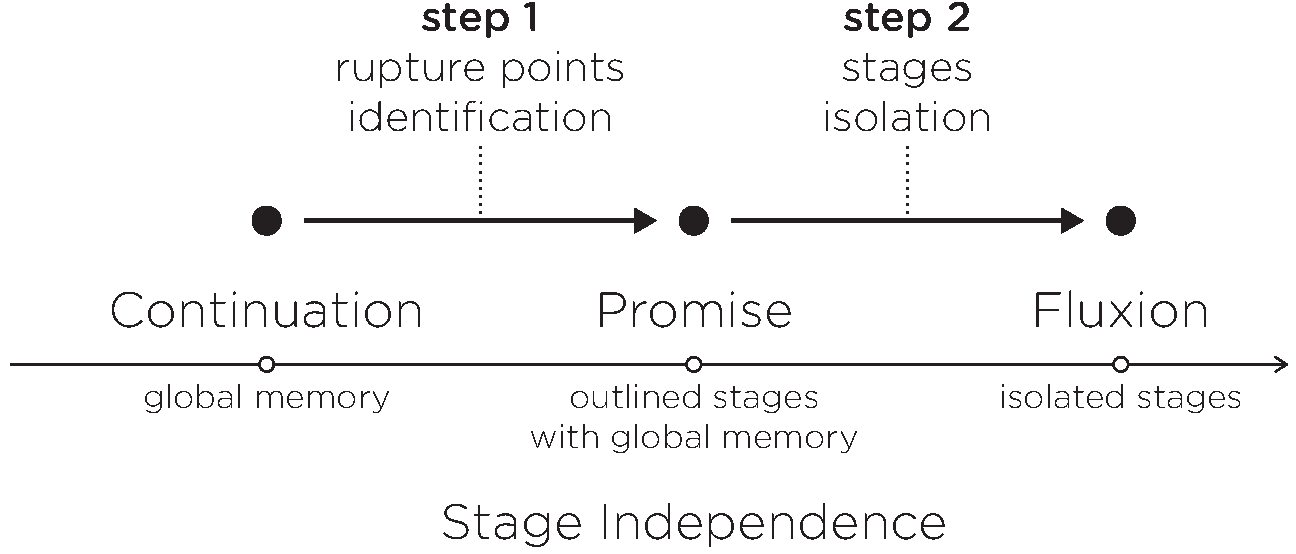
\includegraphics[width=0.7\textwidth]{../resources/roadmap.pdf}%
    \caption{Roadmap}%
    \label{fig:roadmap}%
  }%
\end{figure}

The first compiler focuses on the identification of simple chains of causality between continuations to transform these chains into Promises.
% the transformation from continuations to Promises.
% It focuses on the identification of the chains of causality in continuations.
However, promises are more expressive than the simple chaining of causal sequentiality.
% They force another control over the execution flow.
% According to the outcome of the operation, they call one function to continue the execution with the result, or another to handle errors.
% This conditional execution is indivisible from the Promise specification.
% Promises impose a convention on how to hand back the outcome of the deferred computation, while classic continuations leave this conditional execution to the developer.
Moreover, they impose a different convention than continuations on how to hand back the outcome and errors of the deferred computation.
This difference brings unnecessary complexity to the identification of chains.
To rule out this difference between continuations and Promises, before introducing the first compiler, section \ref{chapter5:due} introduces a simpler specification to Promise, called Due.

The second compiler detects all the chains of causality between continuations and encapsulate them in fluxions.
It isolates the fluxions when possible to allow the parallelism required for efficiency.
This second compilers is introduced in section \ref{chapter5:flx}.

\renewcommand{\glyph}{\iconfont{\XeTeXglyph287}}
\chapter{Implementations} \label{chapter5}
\minitoc
\eject
The transformation allowed by the equivalence from an event-driven program into a distributed network of fluxions is implemented incrementally into two compilers, as presented in figure \ref{fig:roadmap}.
Each compilers is divided into two steps, the identification of the rupture points separating the stages of the pipeline, and the isolation of these stages.
% This chapter presents the technical implementations of these two steps in the transformation from the event-driven execution model to the pipeline architecture
% , the transformation described in the previous chapter was implemented incrementally in two compilers.

\begin{figure}[h!]%
  \textfig{%
    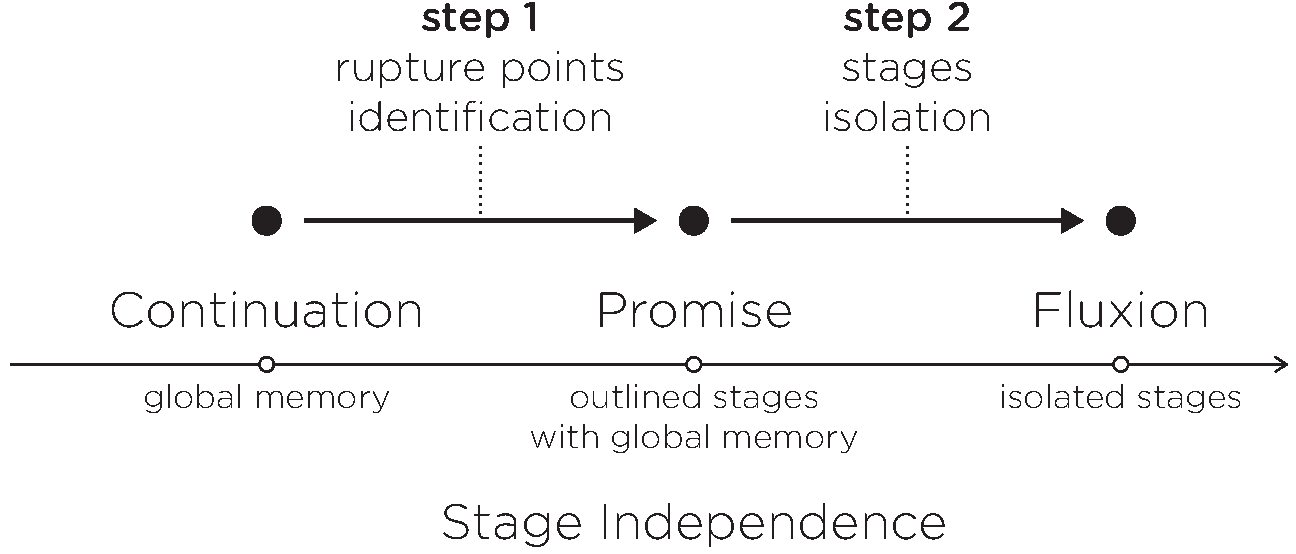
\includegraphics[width=0.7\textwidth]{../resources/roadmap.pdf}%
    \caption{Roadmap}%
    \label{fig:roadmap}%
  }%
\end{figure}

The first compiler focuses on the identification of simple chains of causality between continuations to transform these chains into Promises.
% the transformation from continuations to Promises.
% It focuses on the identification of the chains of causality in continuations.
However, promises are more expressive than the simple chaining of causal sequentiality.
% They force another control over the execution flow.
% According to the outcome of the operation, they call one function to continue the execution with the result, or another to handle errors.
% This conditional execution is indivisible from the Promise specification.
% Promises impose a convention on how to hand back the outcome of the deferred computation, while classic continuations leave this conditional execution to the developer.
Moreover, they impose a different convention than continuations on how to hand back the outcome and errors of the deferred computation.
This difference brings unnecessary complexity to the identification of chains.
To rule out this difference between continuations and Promises, before introducing the first compiler, section \ref{chapter5:due} introduces a simpler specification to Promise, called Due.

The second compiler detects all the chains of causality between continuations and encapsulate them in fluxions.
It isolates the fluxions when possible to allow the parallelism required for efficiency.
This second compilers is introduced in section \ref{chapter5:flx}.

\input{05-implementation/Due/main}
\input{05-implementation/Flx/main}
% \input{05-implementation/Evaluation}

\renewcommand{\glyph}{\iconfont{\XeTeXglyph287}}
\chapter{Implementations} \label{chapter5}
\minitoc
\eject
The transformation allowed by the equivalence from an event-driven program into a distributed network of fluxions is implemented incrementally into two compilers, as presented in figure \ref{fig:roadmap}.
Each compilers is divided into two steps, the identification of the rupture points separating the stages of the pipeline, and the isolation of these stages.
% This chapter presents the technical implementations of these two steps in the transformation from the event-driven execution model to the pipeline architecture
% , the transformation described in the previous chapter was implemented incrementally in two compilers.

\begin{figure}[h!]%
  \textfig{%
    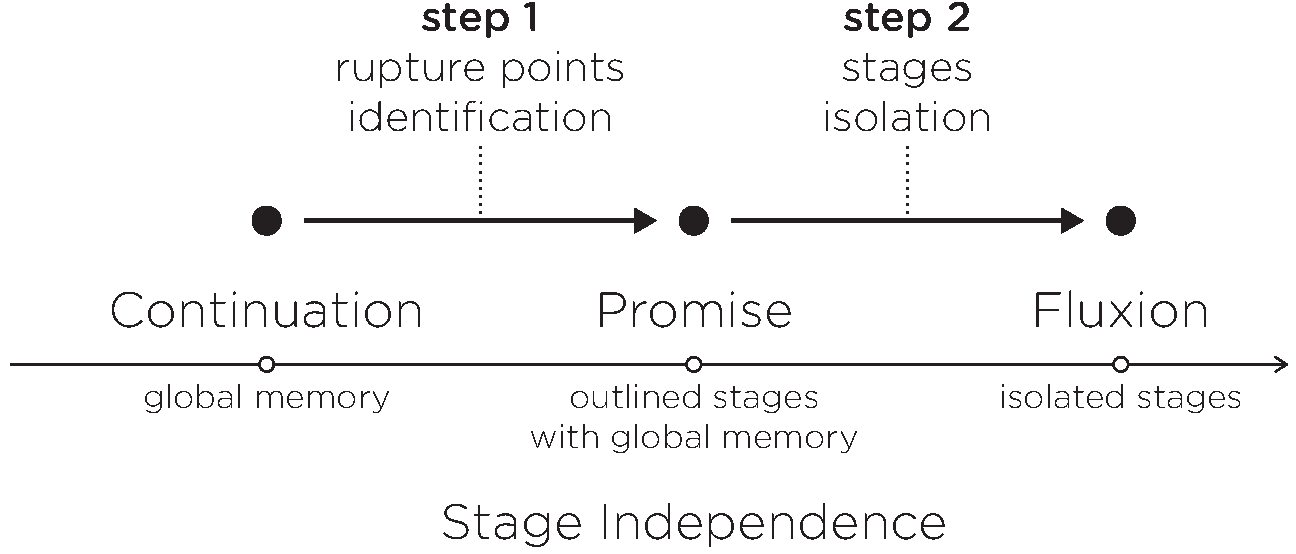
\includegraphics[width=0.7\textwidth]{../resources/roadmap.pdf}%
    \caption{Roadmap}%
    \label{fig:roadmap}%
  }%
\end{figure}

The first compiler focuses on the identification of simple chains of causality between continuations to transform these chains into Promises.
% the transformation from continuations to Promises.
% It focuses on the identification of the chains of causality in continuations.
However, promises are more expressive than the simple chaining of causal sequentiality.
% They force another control over the execution flow.
% According to the outcome of the operation, they call one function to continue the execution with the result, or another to handle errors.
% This conditional execution is indivisible from the Promise specification.
% Promises impose a convention on how to hand back the outcome of the deferred computation, while classic continuations leave this conditional execution to the developer.
Moreover, they impose a different convention than continuations on how to hand back the outcome and errors of the deferred computation.
This difference brings unnecessary complexity to the identification of chains.
To rule out this difference between continuations and Promises, before introducing the first compiler, section \ref{chapter5:due} introduces a simpler specification to Promise, called Due.

The second compiler detects all the chains of causality between continuations and encapsulate them in fluxions.
It isolates the fluxions when possible to allow the parallelism required for efficiency.
This second compilers is introduced in section \ref{chapter5:flx}.

\input{05-implementation/Due/main}
\input{05-implementation/Flx/main}
% \input{05-implementation/Evaluation}

% \subsection{Real test case} \label{chapter5:flx:evaluation}

The compiler is tested on a real application, gifsockets-server\ftnt{https://github.com/twolfson/gifsockets-server}.
This test proves the possibility for an application to be compiled into a network of independent parts.
It shows the current limitations of this isolation and the modifications needed on the application to circumvent them.

\begin{code}[js, caption={Simplified version of gifsockets-server},label={lst:gifsocket}]
var express = require('express'),
    app = express(),
    routes = require('gifsockets-middleware'), //@\label{lst:gifsocket:gif-mw}@
    getRawBody = require('raw-body');

function bodyParser(limit) { //@\label{lst:gifsocket:bodyParser}@
  return function saveBody(req, res, next) { //@\label{lst:gifsocket:saveBody}@
    getRawBody(req, { //@\label{lst:gifsocket:getRawBody}@
      expected: req.headers['content-length'],
      limit: limit
    }, function (err, buffer) { //@\label{lst:gifsocket:callback}@
      req.body = buffer;
      next(); //@\label{lst:gifsocket:next}@
    });
  };
}

app.post('/image/text', bodyParser(1 * 1024 * 1024), routes.writeTextToImages); //@\label{lst:gifsocket:app.post}@
app.listen(8000);
\end{code}

This application, simplified in listing \ref{lst:gifsocket}, is a real-time chat using gif-based communication channels.
It was selected from the evaluation set of the Due compiler because it is simple enough to illustrate this evaluation.
% \cite{Brodu2015}
%  from the \texttt{npm} registry because it depends on \texttt{express}, it is tested, working, and simple enough to illustrate this evaluation.
The server transforms the received text into a gif frame, and pushes it back to a never-ending gif to be displayed on the client.

On line \ref{lst:gifsocket:app.post}, the application registers two functions to process the requests received on the url \texttt{/image/text}.
The closure \texttt{saveBody}, line \ref{lst:gifsocket:saveBody}, returned by \texttt{bodyParser}, line \ref{lst:gifsocket:bodyParser}, and the method \texttt{routes.write\-Text\-To\-Images} from the external module \texttt{gifsockets-\-middleware}, line \ref{lst:gifsocket:gif-mw}.
The closure \texttt{saveBody} calls the asynchronous function \texttt{getRawBody} to get the request body.
Its callback handles the errors, and calls \texttt{next} to continue processing the request with the next function, \texttt{routes.write\-Text\-To\-Images}.

\subsubsection{Compilation} \label{chapter5:flx:evaluation:compilation}

% We compile this application with the compiler
The compilation result is in listing \ref{lst:flx-gifsocket}.
The function call \texttt{app.post}, line \ref{lst:gifsocket:app.post}, is a rupture point.
However, its callbacks, \texttt{bodyParser} and \texttt{routes.write\-Text\-To\-Images} are not declared \textit{in situ}.
They are evaluated as functions only at runtime.
As precised previously, the compiler discards these callbacks to avoid altering the semantic. % by moving or modifying their definition.
% For this reason, the compiler ignores this rupture point, to avoid interfering with the evaluation.

\begin{code}[flx, caption={Compilation result of gifsockets-server},label={lst:flx-gifsocket}]
flx main & express {req}
>> anonymous_1000 [req, next]
  var express = require('express'),
      app = express(),
      routes = require('gifsockets-middleware'), //@\label{lst:flx-gifsocket:gif-mw}@
      getRawBody = require('raw-body');

  function bodyParser(limit) { //@\label{lst:flx-gifsocket:bodyParser}@
    return function saveBody(req, res, next) { //@\label{lst:flx-gifsocket:saveBody}@
      getRawBody(req, { //@\label{lst:flx-gifsocket:getRawBody}@
        expected: req.headers['content-length'], //@\label{lst:flx-gifsocket:req.headers}@
        limit: limit
      }, >> anonymous_1000 [req, next]);
    };
  }

  app.post('/image/text', bodyParser(1 * 1024 * 1024), routes.writeTextToImages); //@\label{lst:flx-gifsocket:app.post}@
  app.listen(8000);

flx anonymous_1000
-> null
  function (err, buffer) { //@\label{lst:flx-gifsocket:callback}@
    req.body = buffer; //@\label{lst:flx-gifsocket:buffer}@
    next(); //@\label{lst:flx-gifsocket:next}@
  }
\end{code}

The compiler detects a rupture point : the function \texttt{get\-Raw\-Body} and its anonymous callback, line \ref{lst:gifsocket:callback}.
It encapsulates this callback in a fluxion named \texttt{anony\-mous\_\-1000}.
The callback is replaced with a stream placeholder to send the message stream to this downstream fluxion.
The variables \texttt{req} and \texttt{next} are appended to this message stream, to propagate their value from the \texttt{main} fluxion to the \texttt{anony\-mous\_\-1000} fluxion.

When \texttt{anony\-mous\_\-1000} is not isolated from the \texttt{main} fluxion, as if they belong to the same group, the compilation result works as expected.
The variables used in the fluxion, \texttt{req} and \texttt{next}, are still shared between the two fluxions.
In this situation fluxions are quite similar to Dues regarding memory shareing.
Our goal is to isolate the two fluxions, to be able to safely parallelize their executions.

\subsubsection{Isolation} \label{chapter5:flx:evaluation:isolation}

In listing \ref{lst:flx-gifsocket}, the fluxion \texttt{anony\-mous\_\-1000} modifies the object \texttt{req}, line \ref{lst:flx-gifsocket:buffer}, to store the text of the received request, and it calls \texttt{next} to continue the execution, line \ref{lst:flx-gifsocket:next}.
\texttt{req} is an alias to a memory location used in multiple palces in code.
Therefore, these operations produce side-effects that should propagate in the whole application, but the isolation prevents this propagation.
Isolating the fluxion \texttt{anony\-mous\_\-1000} produces runtime exceptions.
The next paragraph details how this situation is handled to allow the application to be parallelized.

\paragraph{Variable \texttt{req}}

The variable \texttt{req} is read in fluxion \texttt{main}, lines \ref{lst:flx-gifsocket:getRawBody} and \ref{lst:flx-gifsocket:req.headers}.
Then its property \texttt{body} is associated to \texttt{buffer} in fluxion \texttt{anony\-mous\_\-1000}, line \ref{lst:flx-gifsocket:buffer}.
The compiler is unable to identify the aliases of this variable. % further usages.
However, the side effect resulting from this association impacts a variable in the scope of the next callback, \texttt{routes.write\-Text\-To\-Images}.
In this test case, the application is modified manually to explicitly propagate this side-effect to the next callback through the function \texttt{next}.
The modifications of this function are explained further in the next paragraph.

\paragraph{Closure \texttt{next}}

The function \texttt{next} is a closure provided by the \texttt{express} \texttt{Router} to continue the execution with the next function to handle the client request.
Because it indirectly relies on the variable \texttt{req}, it is impossible to isolate its execution with the \texttt{anony\-mous\_\-1000} fluxion.
Instead, we modify \texttt{express}, so as to be compatible with the fluxional execution model.
We explain the modifications below.

\begin{code}[flx, caption={Simplified modification on the compiled result},label={lst:mflx-gifsocket}]
flx anonymous_1000
-> express_dispatcher
  function (err, buffer) { //@\label{lst:mflx-gifsocket:callback}@
    req.body = buffer; //@\label{lst:mflx-gifsocket:buffer}@
    next_placeholder(req, -> express_dispatcher); //@\label{lst:mflx-gifsocket:next-placeholder}@
  }

flx express_dispatcher & express {req} //@\label{lst:mflx-gifsocket:express-dispatcher}@
-> null
  function (modified_req) {
    merge(req, modified_req);
    next(); //@\label{lst:mflx-gifsocket:next}@
  }
\end{code}

In listing \ref{lst:gifsocket}, the function \texttt{next} is a continuation allowing the anonymous callback, line \ref{lst:gifsocket:callback}, to call the next function to handle the request.
To isolate the anonymous callback into \texttt{anonymous\_\-1000}, \texttt{next} is replaced by a rupture point.
This replacement is illustrated in listing \ref{lst:mflx-gifsocket}.
The \texttt{express} \texttt{Router} registers a fluxion named \texttt{express\_\-dispatcher}, line \ref{lst:mflx-gifsocket:express-dispatcher}, to continue the execution after the fluxion \texttt{anony\-mous\_\-1000}.
This fluxion is in the same group \texttt{express} as the \texttt{main} fluxion, hence it has access to the original variable \texttt{req}, and to the original function \texttt{next}.
The call to the original \texttt{next} function is replaced by a placeholder to push the stream to the fluxion \texttt{express\_\-dispatcher}, line \ref{lst:mflx-gifsocket:next-placeholder}.
The fluxion \texttt{express\_\-dispatcher} receives the stream from the upstream fluxion \texttt{anony\-mous\_\-1000}, merges back the modification in the variable \texttt{req} to propagate the side effects, and finally calls the original function \texttt{next} to continue the execution, line \ref{lst:mflx-gifsocket:next}.

After the modifications detailed above, the server works as expected.
The isolated fluxion correctly receives, and returns its serialized messages.
The client successfully receives a gif frame containing the text.



\subsection{Limitations}

The static analysis used for this compiler presents some limitations.
It is unable to analyze code with dynamic behaviors.
Higher-order programming leads to more productivity partly beacuse it rely on such dynamic behavior to extend expressivity.
Precisely, it allows more levels of indirections.

\subsubsection{Levels of Indirections}

The indirection is an abstraction between the value, and its manipulation.
In listing \ref{lst:indirection}, the variables \texttt{a} and \texttt{b} point both to the same memory object.
The function \texttt{fn} introduces a level of indirection between the real object \texttt{a} and its manipulation handle, \texttt{b};
% Actually, the variable \texttt{a} already introduces a level of indirection between the real object and the handle \texttt{a}.

\begin{code}[js,
  caption={One level of Indirection},
  label={lst:indirection}]
var a = {
      // an object;
    };

fn(b) {
  // modify b;
}

fn(a);
\end{code}

\subsubsection{Uncertainties}

The indirection is trivial to resolve in listing \ref{lst:indirection}.
It only needs to have access to the definition of \texttt{a} and of \texttt{fn}.
%A very simple static analysis could resolve it.
However, in listing \ref{lst:indirections}, the array \texttt{handlers} introduces a new level of indirection.
The static analysis now needs to have access to the definition of \texttt{i} and of the \texttt{handlers}.
If this definition is provided by an external input, it is not available statically, hence, it adds an uncertainty during the analysis. 

\begin{code}[js,
  caption={Two levels of indirection},
  label={lst:indirections}]
var a = {
      // an object;
    },
    handlers = [
      // definition of fn handlers;
    ],
    i = ?;

handlers[i](a);
handlers[i+1](a);
\end{code}

These examples are extremely simplified.
A real application contains enough indirections for the static analysis to be overwhelmed by uncertainties, and to be unable to resolve the variables.
If a variable is left unresolved, it is impossible to assure its scope and its aliases.
Therefore, the compiler is unable to isolate it into a fluxion, or to distribute its modification by messages.

Moreover, it leads the compiler to ignore the rupture points not defined \textit{in situ}, because their modifications could impact the semantic.
The reason for this precaution, is that the compiler is unable to assure where the function is used, and the scope of its variables.
Therefore, it is unable to assure that the modification will conserve the semantic.

\subsubsection{Dynamic Resolution}

In a web application, this variable \texttt{i} might be part of the user request, which is available only at runtime.
It eventually introduces an uncertainty.

This dynamic resolution of variables is precisely what increase expressiveness.
Trying to resolve them statically is equivalent to restrict expressiveness.
No static analysis can overstep these limitations.
Only a dynamic analysis could analysis the resolved indirections during run time to overstep these limitations correctly.




% \subsection{Real test case} \label{chapter5:flx:evaluation}

The compiler is tested on a real application, gifsockets-server\ftnt{https://github.com/twolfson/gifsockets-server}.
This test proves the possibility for an application to be compiled into a network of independent parts.
It shows the current limitations of this isolation and the modifications needed on the application to circumvent them.

\begin{code}[js, caption={Simplified version of gifsockets-server},label={lst:gifsocket}]
var express = require('express'),
    app = express(),
    routes = require('gifsockets-middleware'), //@\label{lst:gifsocket:gif-mw}@
    getRawBody = require('raw-body');

function bodyParser(limit) { //@\label{lst:gifsocket:bodyParser}@
  return function saveBody(req, res, next) { //@\label{lst:gifsocket:saveBody}@
    getRawBody(req, { //@\label{lst:gifsocket:getRawBody}@
      expected: req.headers['content-length'],
      limit: limit
    }, function (err, buffer) { //@\label{lst:gifsocket:callback}@
      req.body = buffer;
      next(); //@\label{lst:gifsocket:next}@
    });
  };
}

app.post('/image/text', bodyParser(1 * 1024 * 1024), routes.writeTextToImages); //@\label{lst:gifsocket:app.post}@
app.listen(8000);
\end{code}

This application, simplified in listing \ref{lst:gifsocket}, is a real-time chat using gif-based communication channels.
It was selected from the evaluation set of the Due compiler because it is simple enough to illustrate this evaluation.
% \cite{Brodu2015}
%  from the \texttt{npm} registry because it depends on \texttt{express}, it is tested, working, and simple enough to illustrate this evaluation.
The server transforms the received text into a gif frame, and pushes it back to a never-ending gif to be displayed on the client.

On line \ref{lst:gifsocket:app.post}, the application registers two functions to process the requests received on the url \texttt{/image/text}.
The closure \texttt{saveBody}, line \ref{lst:gifsocket:saveBody}, returned by \texttt{bodyParser}, line \ref{lst:gifsocket:bodyParser}, and the method \texttt{routes.write\-Text\-To\-Images} from the external module \texttt{gifsockets-\-middleware}, line \ref{lst:gifsocket:gif-mw}.
The closure \texttt{saveBody} calls the asynchronous function \texttt{getRawBody} to get the request body.
Its callback handles the errors, and calls \texttt{next} to continue processing the request with the next function, \texttt{routes.write\-Text\-To\-Images}.

\subsubsection{Compilation} \label{chapter5:flx:evaluation:compilation}

% We compile this application with the compiler
The compilation result is in listing \ref{lst:flx-gifsocket}.
The function call \texttt{app.post}, line \ref{lst:gifsocket:app.post}, is a rupture point.
However, its callbacks, \texttt{bodyParser} and \texttt{routes.write\-Text\-To\-Images} are not declared \textit{in situ}.
They are evaluated as functions only at runtime.
As precised previously, the compiler discards these callbacks to avoid altering the semantic. % by moving or modifying their definition.
% For this reason, the compiler ignores this rupture point, to avoid interfering with the evaluation.

\begin{code}[flx, caption={Compilation result of gifsockets-server},label={lst:flx-gifsocket}]
flx main & express {req}
>> anonymous_1000 [req, next]
  var express = require('express'),
      app = express(),
      routes = require('gifsockets-middleware'), //@\label{lst:flx-gifsocket:gif-mw}@
      getRawBody = require('raw-body');

  function bodyParser(limit) { //@\label{lst:flx-gifsocket:bodyParser}@
    return function saveBody(req, res, next) { //@\label{lst:flx-gifsocket:saveBody}@
      getRawBody(req, { //@\label{lst:flx-gifsocket:getRawBody}@
        expected: req.headers['content-length'], //@\label{lst:flx-gifsocket:req.headers}@
        limit: limit
      }, >> anonymous_1000 [req, next]);
    };
  }

  app.post('/image/text', bodyParser(1 * 1024 * 1024), routes.writeTextToImages); //@\label{lst:flx-gifsocket:app.post}@
  app.listen(8000);

flx anonymous_1000
-> null
  function (err, buffer) { //@\label{lst:flx-gifsocket:callback}@
    req.body = buffer; //@\label{lst:flx-gifsocket:buffer}@
    next(); //@\label{lst:flx-gifsocket:next}@
  }
\end{code}

The compiler detects a rupture point : the function \texttt{get\-Raw\-Body} and its anonymous callback, line \ref{lst:gifsocket:callback}.
It encapsulates this callback in a fluxion named \texttt{anony\-mous\_\-1000}.
The callback is replaced with a stream placeholder to send the message stream to this downstream fluxion.
The variables \texttt{req} and \texttt{next} are appended to this message stream, to propagate their value from the \texttt{main} fluxion to the \texttt{anony\-mous\_\-1000} fluxion.

When \texttt{anony\-mous\_\-1000} is not isolated from the \texttt{main} fluxion, as if they belong to the same group, the compilation result works as expected.
The variables used in the fluxion, \texttt{req} and \texttt{next}, are still shared between the two fluxions.
In this situation fluxions are quite similar to Dues regarding memory shareing.
Our goal is to isolate the two fluxions, to be able to safely parallelize their executions.

\subsubsection{Isolation} \label{chapter5:flx:evaluation:isolation}

In listing \ref{lst:flx-gifsocket}, the fluxion \texttt{anony\-mous\_\-1000} modifies the object \texttt{req}, line \ref{lst:flx-gifsocket:buffer}, to store the text of the received request, and it calls \texttt{next} to continue the execution, line \ref{lst:flx-gifsocket:next}.
\texttt{req} is an alias to a memory location used in multiple palces in code.
Therefore, these operations produce side-effects that should propagate in the whole application, but the isolation prevents this propagation.
Isolating the fluxion \texttt{anony\-mous\_\-1000} produces runtime exceptions.
The next paragraph details how this situation is handled to allow the application to be parallelized.

\paragraph{Variable \texttt{req}}

The variable \texttt{req} is read in fluxion \texttt{main}, lines \ref{lst:flx-gifsocket:getRawBody} and \ref{lst:flx-gifsocket:req.headers}.
Then its property \texttt{body} is associated to \texttt{buffer} in fluxion \texttt{anony\-mous\_\-1000}, line \ref{lst:flx-gifsocket:buffer}.
The compiler is unable to identify the aliases of this variable. % further usages.
However, the side effect resulting from this association impacts a variable in the scope of the next callback, \texttt{routes.write\-Text\-To\-Images}.
In this test case, the application is modified manually to explicitly propagate this side-effect to the next callback through the function \texttt{next}.
The modifications of this function are explained further in the next paragraph.

\paragraph{Closure \texttt{next}}

The function \texttt{next} is a closure provided by the \texttt{express} \texttt{Router} to continue the execution with the next function to handle the client request.
Because it indirectly relies on the variable \texttt{req}, it is impossible to isolate its execution with the \texttt{anony\-mous\_\-1000} fluxion.
Instead, we modify \texttt{express}, so as to be compatible with the fluxional execution model.
We explain the modifications below.

\begin{code}[flx, caption={Simplified modification on the compiled result},label={lst:mflx-gifsocket}]
flx anonymous_1000
-> express_dispatcher
  function (err, buffer) { //@\label{lst:mflx-gifsocket:callback}@
    req.body = buffer; //@\label{lst:mflx-gifsocket:buffer}@
    next_placeholder(req, -> express_dispatcher); //@\label{lst:mflx-gifsocket:next-placeholder}@
  }

flx express_dispatcher & express {req} //@\label{lst:mflx-gifsocket:express-dispatcher}@
-> null
  function (modified_req) {
    merge(req, modified_req);
    next(); //@\label{lst:mflx-gifsocket:next}@
  }
\end{code}

In listing \ref{lst:gifsocket}, the function \texttt{next} is a continuation allowing the anonymous callback, line \ref{lst:gifsocket:callback}, to call the next function to handle the request.
To isolate the anonymous callback into \texttt{anonymous\_\-1000}, \texttt{next} is replaced by a rupture point.
This replacement is illustrated in listing \ref{lst:mflx-gifsocket}.
The \texttt{express} \texttt{Router} registers a fluxion named \texttt{express\_\-dispatcher}, line \ref{lst:mflx-gifsocket:express-dispatcher}, to continue the execution after the fluxion \texttt{anony\-mous\_\-1000}.
This fluxion is in the same group \texttt{express} as the \texttt{main} fluxion, hence it has access to the original variable \texttt{req}, and to the original function \texttt{next}.
The call to the original \texttt{next} function is replaced by a placeholder to push the stream to the fluxion \texttt{express\_\-dispatcher}, line \ref{lst:mflx-gifsocket:next-placeholder}.
The fluxion \texttt{express\_\-dispatcher} receives the stream from the upstream fluxion \texttt{anony\-mous\_\-1000}, merges back the modification in the variable \texttt{req} to propagate the side effects, and finally calls the original function \texttt{next} to continue the execution, line \ref{lst:mflx-gifsocket:next}.

After the modifications detailed above, the server works as expected.
The isolated fluxion correctly receives, and returns its serialized messages.
The client successfully receives a gif frame containing the text.



\subsection{Limitations}

The static analysis used for this compiler presents some limitations.
It is unable to analyze code with dynamic behaviors.
Higher-order programming leads to more productivity partly beacuse it rely on such dynamic behavior to extend expressivity.
Precisely, it allows more levels of indirections.

\subsubsection{Levels of Indirections}

The indirection is an abstraction between the value, and its manipulation.
In listing \ref{lst:indirection}, the variables \texttt{a} and \texttt{b} point both to the same memory object.
The function \texttt{fn} introduces a level of indirection between the real object \texttt{a} and its manipulation handle, \texttt{b};
% Actually, the variable \texttt{a} already introduces a level of indirection between the real object and the handle \texttt{a}.

\begin{code}[js,
  caption={One level of Indirection},
  label={lst:indirection}]
var a = {
      // an object;
    };

fn(b) {
  // modify b;
}

fn(a);
\end{code}

\subsubsection{Uncertainties}

The indirection is trivial to resolve in listing \ref{lst:indirection}.
It only needs to have access to the definition of \texttt{a} and of \texttt{fn}.
%A very simple static analysis could resolve it.
However, in listing \ref{lst:indirections}, the array \texttt{handlers} introduces a new level of indirection.
The static analysis now needs to have access to the definition of \texttt{i} and of the \texttt{handlers}.
If this definition is provided by an external input, it is not available statically, hence, it adds an uncertainty during the analysis. 

\begin{code}[js,
  caption={Two levels of indirection},
  label={lst:indirections}]
var a = {
      // an object;
    },
    handlers = [
      // definition of fn handlers;
    ],
    i = ?;

handlers[i](a);
handlers[i+1](a);
\end{code}

These examples are extremely simplified.
A real application contains enough indirections for the static analysis to be overwhelmed by uncertainties, and to be unable to resolve the variables.
If a variable is left unresolved, it is impossible to assure its scope and its aliases.
Therefore, the compiler is unable to isolate it into a fluxion, or to distribute its modification by messages.

Moreover, it leads the compiler to ignore the rupture points not defined \textit{in situ}, because their modifications could impact the semantic.
The reason for this precaution, is that the compiler is unable to assure where the function is used, and the scope of its variables.
Therefore, it is unable to assure that the modification will conserve the semantic.

\subsubsection{Dynamic Resolution}

In a web application, this variable \texttt{i} might be part of the user request, which is available only at runtime.
It eventually introduces an uncertainty.

This dynamic resolution of variables is precisely what increase expressiveness.
Trying to resolve them statically is equivalent to restrict expressiveness.
No static analysis can overstep these limitations.
Only a dynamic analysis could analysis the resolved indirections during run time to overstep these limitations correctly.





\printbibliography[]

\end{document}